\documentclass[french]{report}
\usepackage[utf8]{inputenc}
\usepackage[T1]{fontenc}
\usepackage{lmodern}
\usepackage[a4paper]{geometry}
\usepackage[francais]{babel}
\usepackage{amsmath}
\usepackage{gensymb}
\usepackage{amsfonts}
\usepackage{amssymb}
\usepackage{sidecap}
\usepackage{xfrac}
\usepackage{caption}
\usepackage{hyperref}
\usepackage{afterpage}
\usepackage{soul}
\usepackage[bottom]{footmisc}
\usepackage{tikz}
\usepackage{boxedminipage}
\usepackage{chngcntr}
\usepackage{comment}
\usepackage{placeins} %\FloatBarrier
\counterwithout{equation}{chapter}
\counterwithout{figure}{chapter}
\usepackage{titlesec}
\usepackage{changepage}% http://ctan.org/pkg/changepage
 \usepackage{enumitem}

\usetikzlibrary{decorations}
\usepackage{subcaption}
%%%%%%%%%%%%%%%%%%%%%%%%%%%%%%%%%%%
\tikzset{
bicolor/.style 2 args={
  thick,dashed,dash pattern=on 6pt off 6pt,-,#1,
  postaction={draw,dashed,dash pattern=on 4pt off 8pt,-,#2,dash phase=5pt}
  },
}
%%%%%%%%%%%%%%%%%%%%%%%%%%%%%%%%%%%

%%%%%%%%%%%%%%%%%%%%%%%%%%%%%%%%%%%
%\titlespacing{\chapter} {0pt} {*0} {*0} {} 
%\titlespacing{\section} {0ex} {*0} {*0} {} 
%\titlespacing{\subsection} {0ex} {*0} {*0} {} 
%\titlespacing{\subsubsection} {10ex} {8ex} {*0} {} 

\begin{document}

	\def \axeline {dotted}
	\def\changemargin#1#2{\list{}{\rightmargin#2\leftmargin#1}\item[]}
	%\newcommand*{\Line}[3][]{\tikz \draw[#1] #2 -- #3;}
	\let\endchangemargin=\endlist 

\definecolor{b}{RGB}{100,150,200}
\definecolor{v}{RGB}{120,200,80}
\definecolor{r}{RGB}{220,80,70}
\definecolor{j}{RGB}{255,220,50}
\definecolor{f}{RGB}{180,80,180}
\definecolor{w}{RGB}{255,255,255}
\definecolor{n}{RGB}{0,0,0}

\begin{titlepage}
\begin{center}
\textit{}\vfill

\textit{}\\\textit{}\\\textit{}\\\textit{}\\
\today\\[0.8cm]
%\LARGE{\textsc{Université Libre de Bruxelles}}\\
%\LARGE{\textsc{Université Libre de Bruxelles}}\\
%\LARGE{Faculté des Sciences} \large{· Département de Physique}\\[0.8cm]

\rule{\linewidth}{.5pt}\\[1.0cm]

%{ \large {Mémoire présenté en vue de l'obtention\\du diplôme de Master en Sciences Physiques}}\\[0.8cm]
%{ \Huge \bfseries Magnétosphères\\autour de trous-noirs}\\[0.8cm]
{ \Huge \bfseries Théorème des Quatre Couleurs}\\[0.8cm]
%\Large{Travail dirigé par M. Geoffrey \textsc{Compère}}\\
%{\large Physique Théorique Mathématique}\\[0.2cm]

\rule{\linewidth}{.5pt} \\[1.2cm]

\LARGE{Éric \& Noé \textsc{Vandevoorde}}\\
%\large{avec l'aide de Noé \textsc{Vandevoorde}}
%\large{Année académique 2015·2016}

\vfill\textit{}
\end{center}
\end{titlepage}

\newpage
\pagenumbering{gobble}

\tableofcontents

\chapter{Introduction}

\pagenumbering{arabic}
\setcounter{page}{2}
%\noindent
%\parindent=0cm

%${\mathcal{C}}_{53}$\\
%$\overline{\mathcal{C}}_{53}$\\
%${\mathcal{PC}}_{53}$\\

Le but de ce document est de démontrer que quatre couleurs suffisent pour colorier n'importe quelle carte géographique et dès lors que tout graphe simple, planaire et connexe est de nombre chromatique quatre (voir la section suivante pour la définition de ces critères). Ce résultat est connu sous le nom du \textit{théorème des quatre couleurs}.\bigskip

Le problème remonte à 1852, lorsque le cartographe anglais Francis \textsc{Guthrie} remarqua qu'il lui suffisait de quatre couleurs pour colorer la carte (pourtant complexe) des comtés d'Angleterre, sans que deux cantons voisins ne reçoivent la même couleur. Son frère Frederick, mathématicien, ne parvenant pas à savoir si la propriété était générale, transmit la réflexion à son professeur, Auguste \textsc{de Morgan} de la \textit{University College} de Londres. Et de fil en aiguille, le problème (devenu postulat, puis conjecture), se répandit dans la sphère mathématique, aidé en 1978 par la publication de la question par Arthur \textsc{Cayley} et son évocation lors d'un colloque de la \textit{London Mathematical Society}. Prèsqu'aussitôt, Alfred \textsc{Kempe} propose une preuve de la conjecture en 1879 et, pendant une décennie, on crut le problème des quatre couleurs résolu. \textsc{Kempe} fut élu membre de la \textit{Royal Society} et devint ensuite président de la \textit{London Mathematical Society}. Mais onze ans plus tard, en 1890, Percy John \textsc{Heawood} trouva une faille majeure dans la démonstration. Il parvient cependant à sauvegarder tant bien que mal la preuve en un \textit{théorème des cinq couleurs}. Une seconde preuve, proposée par Peter Guthrie \textsc{Tait} dès 1880, fut également réfutée, par Julius \textsc{Peterson} en 1891.\smallskip

De nombreuses tentatives ont étés introduites pour réduire à quatre le nombre de couleurs à partir de la démonstration de \textsc{Kempe-Heawood}. En 1913, le père de l'algèbre moderne George David \textsc{Birkhoff}, formule une notion de configuration réductible et démontre la conjecture pour toutes les cartes comportant moins de vingt-six régions à colorier et cette borne est petit à petit améliorée au cours du siècle. En 1969, Heinrich \textsc{Heesch} trouve des conditions \textit{presque} nécessaires et suffisantes pour qu'une configuration soit réductible et une méthode générale pour trouver un ensemble de configurations inévitable. Ce n'est finalement qu'en 1976 que la première démonstration complète fut acceptée, celle de Kenneth \textsc{Appel} et Wolfgang \textsc{Haken}. Ces derniers réalisèrent de manière informatique le programme de \textsc{Heesch} et montrèrent, après 1200 heures de calcul et des dizaines de milliers de figures à l'appui, que les 1478 configurations sont réductibles et 4-coloriables. Cette preuve fut la première démonstration acceptée sur base de l'utilisation massive de l'ordinateur. Enfin, en 1995, Neil \textsc{Robertson}, Daniel \textsc{Sanders}, Paul \textsc{Seymour} et Robin \textsc{Thomas} mirent à profit l'avancement de la technologie pour compiler une réalisation nettement plus simple du programme de \textsc{Heesch}, avec seulement 633 configurations.

Dans ce document, nous déclarons exposer une preuve complète du théorème qui ne nécessite pas l'utilisation d'outil informatique.

Notre document est découpé en 3 chapitres.\\
Dans le 1er chapitre, nous donnons les définitions permettant de cadrer notre propos et tout particulièrement la définition du graphe géographique et de la chaine de Kempe.
Dans le 2ème chapitre nous reprenons la démonstration du théorème des cinq couleurs. Ce n'est pas directement notre sujet, mais nous nous basons sur les mêmes principes, il était donc normal de les rappeler. Enfin, le 3ème chapitre s’attaque au théorème des quatre couleurs et à sa résolution.

\section{Carte et coloration}

Pour colorer une carte géographique, on demande que toute paire de pays limitrophes soit coloriée de deux couleurs différentes afin de visualiser clairement la frontière qui sépare les deux pays. Dans le cadre de la démonstration du théorème, nous ne considérerons que des pays connexes, c'est-à-dire constitués d'un seul morceau\footnote{La Corse, l'Alaska ou Baerle-Duc sont dès lors considérés comme des pays indépendants.}. De plus, nous restreindrons la définition de frontière entre deux pays à des courbes de longueur non nulle : deux pays ne se touchant que par un point ne sont pas considérés comme limitrophes. Enfin, nous considérerons que la carte étudiée est constituée d'un nombre fini de pays, regroupés en un ensemble connexe unique (\textit{i.e.}~ nous ne regardons qu'un seul continent).

À toute carte géographique satisfaisant ces hypothèses, on peut associer un \textit{graphe} coloré\footnote{Une coloration d'un graphe $G$ est une fonction associant à tout sommet de $G$ une couleur, généralement un élément de l'ensemble d'indices $\{1, 2, ..., n\}$, telle que deux sommets adjacents n'ont pas la même couleur (où $n$ est le nombre de sommets du graphe). De manière équivalente, en définissant un \textit{stable} de \textit{G} par un sous-ensemble de sommets deux-à-deux non adjacents, une coloration de $G$ est une partition de son ensemble de sommets en stables. On ne différentie généralement pas les colorations qui ne sont distinctes qu'à une permutation des indices de couleurs près.}, c'est-à-dire une représentation schématique des liens entre les pays (voir Figure~\ref{Carte}). Chaque pays est représenté par un \textit{sommet} coloré, relié par des \textit{arrêtes} à ses pays limitrophes. Le nombre de pays limitrophes à un sommet (\textit{i.e.}~le nombre d'arêtes partant de ce sommet) est appelé son \textit{degré}, que l'on note~$d\in\mathbb{N}^+$. Les polygones délimités par les arrêtes entre les sommets sont appelés les \textit{faces} du graphe\footnote{Les équivalents de ces faces dans la carte géographique d'origine pourraient être appelés des \textit{embranchement de frontières}, c'est à dire des points d'où partent au moins trois frontières ou, dit autrement, où au moins trois pays se rencontrent. Ce n'est cependant pas toujours vrai : sur le graphe de la Figure~\ref{Carte} le Liechtenstein et l'Allemagne bordent la même face alors qu'ils ne partagent pas de frontière.}. Précisons tout de suite que l'espace externe délimité par le graphe est toujours considéré comme étant une face\footnote{Un graphe ne comportant qu'un seul sommet et aucune arête possède donc une face.}.

\begin{figure}[b!]\centering{
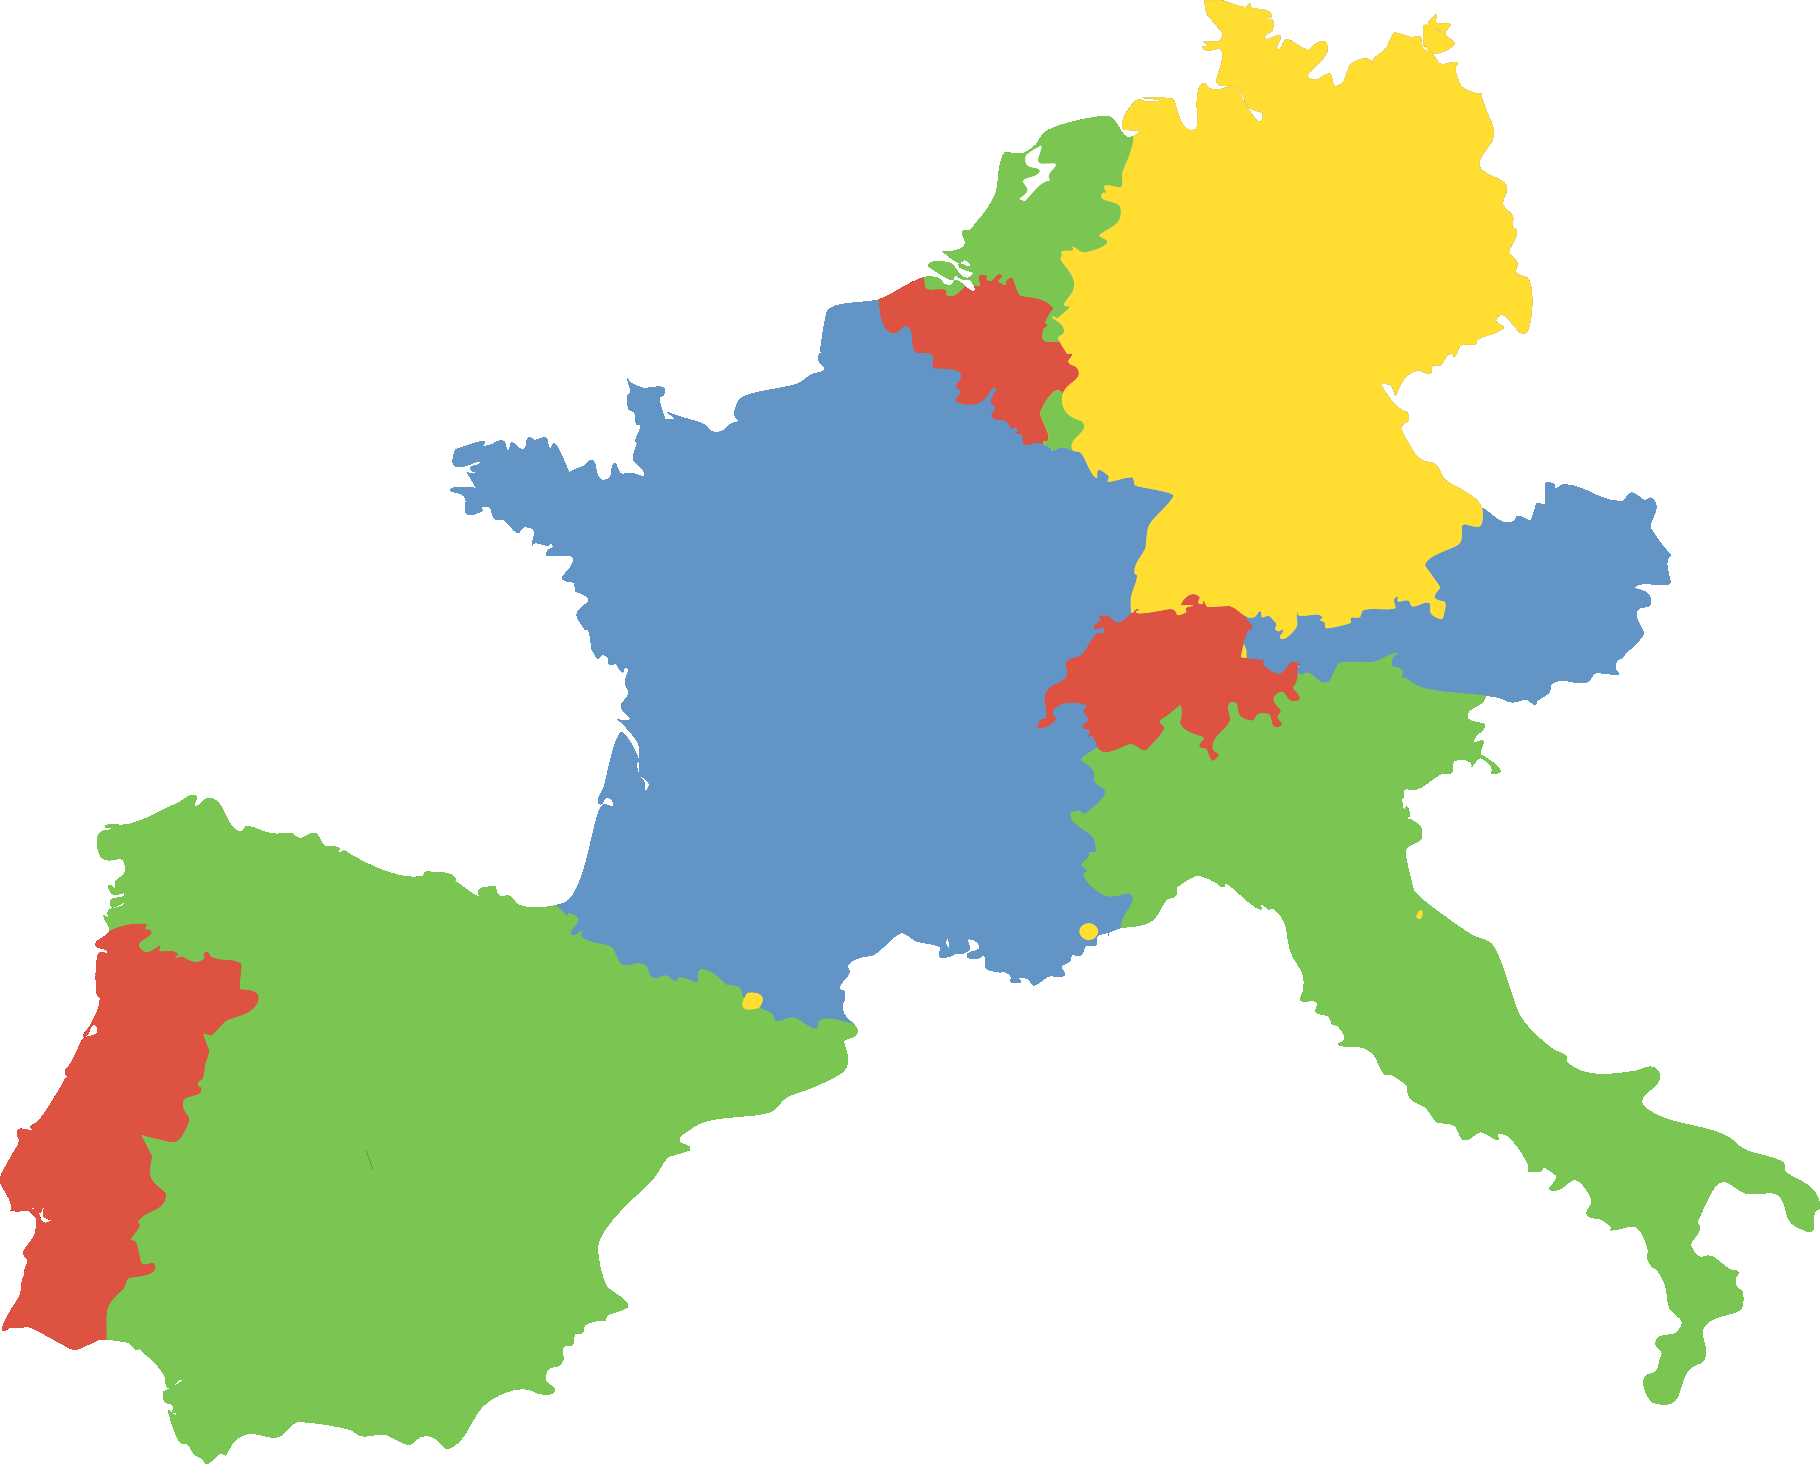
\includegraphics[width=.45\textwidth]{Carte}\qquad
\begin{tikzpicture}[scale=2.0]
\node[draw, circle,minimum size=.7cm,fill=j] (DE) at (3.042,2.736) {\scriptsize{DE}};
\node[draw, circle,minimum size=.7cm,fill=j] (AD) at (1.884,1.301) {\scriptsize{AD}};
\node[draw, circle,minimum size=.7cm,fill=b] (AT) at (3.568,2.019) {\scriptsize{AT}};
\node[draw, circle,minimum size=.7cm,fill=r] (BE) at (2.108,2.847) {\scriptsize{BE}};
\node[draw, circle,minimum size=.7cm,fill=v] (ES) at (1.296,1) {\scriptsize{ES}};
\node[draw, circle,minimum size=.7cm,fill=b] (FR) at (2.025,1.884) {\scriptsize{FR}};
\node[draw, circle,minimum size=.7cm,fill=v] (IT) at (3.042,1.111) {\scriptsize{IT}};
\node[draw, circle,minimum size=.7cm,fill=j] (LI) at (3.078,2.188) {\scriptsize{LI}};
\node[draw, circle,minimum size=.7cm,fill=v] (LU) at (2.409,2.507) {\scriptsize{LU}};
\node[draw, circle,minimum size=.7cm,fill=j] (MC) at (2.353,1.301) {\scriptsize{MC}};
\node[draw, circle,minimum size=.7cm,fill=v] (NL) at (2.460,3.185) {\scriptsize{NL}};
\node[draw, circle,minimum size=.7cm,fill=r] (PT) at (0.796,1) {\scriptsize{PT}};
\node[draw, circle,minimum size=.7cm,fill=j] (SM) at (3.568,1.371) {\scriptsize{SM}};
\node[draw, circle,minimum size=.7cm,fill=r] (CH) at (2.670,1.884) {\scriptsize{CH}};
\node[draw, circle,minimum size=.7cm,fill=r] (VA) at (2.536,0.851) {\scriptsize{VA}};
\path (DE) edge (NL);\path (DE) edge (BE);\path (DE) edge (LU);\path (DE) edge (CH);\path (DE) edge (AT);\path (DE) edge (FR);
\path (AD) edge (FR);\path (AD) edge (ES);
\path (AT) edge (CH);\path (AT) edge (LI);\path (AT) edge (IT);
\path (BE) edge (NL);\path (BE) edge (LU);\path (BE) edge (FR);
\path (ES) edge (PT);\path (ES) edge (FR);
\path (FR) edge (IT);\path (FR) edge (CH);\path (FR) edge (LU);\path (FR) edge (MC);
\path (IT) edge (SM);\path (IT) edge (CH);\path (IT) edge (VA);
\path (LI) edge (CH);
%  \path (2) edge[looseness=1.8,bend left=90] (5);
\end{tikzpicture}
\caption{Exemple de carte géographique et du graphe associé}\label{Carte}}
\end{figure}

Puisque les graphes que nous considérerons proviennent tous de cartes géographiques, ils satisfont aux propriétés suivantes :
%\begin{enumerate}
\begin{description}

\item[\textbf{Simple ·}] Un pays n'ayant pas de frontière avec lui-même, le graphe ne présente pas de boucle (c'est-à-dire d'arête retournant sur le sommet dont elle est issue). De même, une et une seule frontière peut exister entre deux pays (connexes) et il ne peut dès lors y avoir d'arêtes multiples entre deux sommets. On dit d'un graphe sans boucle ni lien multiple qu'il est \textit{simple} ;
\item[\textbf{Planaire ·}] Une frontière ne pouvant se restreindre à un seul point, les arêtes du graphe ne peuvent pas se croiser. De plus, quelque soit la projection utilisée, une carte peut toujours être représentée sur un plan, sans devoir introduire de troisième dimension. Dès lors le graphe associé est également restreint à un plan et un sommet ne peut être relié par un autre en passant \textit{au dessus} d'arêtes ou de sommets. Ainsi, le seul endroit où deux arêtes peuvent se rencontrer est en un sommet. On dit d'un graphe pouvant être représenté sur un plan de façon à ce qu'aucune arête ne se croise qu'il est \textit{planaire} ;
\item[\textbf{Connexe ·}] Tous les pays étant regroupés en un bloc unique (\textit{i.e.}~un continent), tous les sommets sont reliés les uns aux autres par des arêtes et on peut toujours trouver une succession d'arêtes (ce qu'on appelle un \textit{chemin}%\footnote{Lorsqu'on parlera de longueur de chemin et de chemin fermé, on sous-entendra par \textit{succession d'arêtes} qu'on ne passe jamais plus d'une fois par la même arête, quelque soit le sens de parcours.}
) qui relie n'importe quelle paire de sommets. On dit alors que le graphe est \textit{connexe}.
%\end{enumerate}
\end{description}
Tous les graphes que nous considèrerons par la suite seront simples, planaires et connexes. Pour éviter la lourdeur de répétitions continues, nous sous-entendrons ces hypothèses par la dénomination de \textit{graphe géographique}.

\section{Chaine de Kempe}

Dans ce qui suit, nous utiliserons abondamment la notion de \textit{chaine de \textsc{Kempe}}, à laquelle nous ferons référence en parlant simplement de \textit{chaine}. Une chaine de \textsc{Kempe} est un sous-ensemble bicolore connexe d'une carte coloriée. En terme de graphes, une chaine de \textsc{Kempe} est un sous-graphe connexe maximum dichromatique. Remarquons que ces «~chaines~» ne sont pas nécessairement linéaires et peuvent être des arbres ou comprendre des chemins fermés. Dans une chaine (par définition bicolore), on peut toujours échanger les deux couleurs sans que cela ne pose de problème dans le coloriage général de la carte (ou du graphe associé). On notera $\mathcal{C}_{ab}$ la chaine comportant le sommet $a$ et dont la seconde couleur est celle du sommet $b$, celui-ci ne faisant pas nécessairement partie de la chaine (on peut donc avoir $\mathcal{C}_{ab}\cap\mathcal{C}_{ba}=\varnothing$).

Par exemple, sur la Figure~\ref{Carte}, le Benelux forme une chaine verte-rouge que l'on peut noter de plusieurs façons : $\mathcal{C}_{\textsc{be}\cdot\textsc{nl}}=\mathcal{C}_{\textsc{lu}\cdot\textsc{pt}}=...$ . De même, Andorre, Monaco, la France, l'Allemagne, l'Autriche et le Liechtenstein forment une chaine jaune/bleue. Inverser les couleurs jaune et bleue au sein de cette chaine donne une coloration tout aussi valable de la carte et du graphe.

Dans le cas où la chaine $\mathcal{C}_{ab}$ contient à la fois le sommet $a$ et le sommet $b$ (\textit{i.e.} lorsque~$\mathcal{C}_{ab}=\mathcal{C}_{ba}$), on dira que la chaine $a$-$b$ est complète, ce que l'on notera~$\overline{\mathcal{C}}_{ab}$.
%On notera dans la suite du document $\overline{\mathcal{C}}_{xy}$ la chaine commune a «~x~» et «~y~», soit lorsque la $\mathcal{C}_{xy}$ = $\mathcal{C}_{yx}$. 


\chapter{Théorème des cinq couleurs}

Le nombre minimal de couleurs différentes nécessaires pour la coloration d'un graphe est appelé son \textit{nombre chromatique}. Il est relativement aisé de montrer que le nombre chromatique de tout graphe géographique est au plus cinq. Ce résultat est le \textit{théorème des cinq couleurs} : cinq couleurs suffisent toujours pour colorer n'importe quelle carte simple planaire connexe. Nous allons redonner ici une démonstration de ce théorème et nous nous baserons sur ce résultat dans la suite pour montrer que quatre couleurs sont en fait déjà suffisantes.

\section{Formule d'Euler}

Comme échauffement, nous allons commencer par redémontrer que tout graphe associé à une carte géographique satisfait à la \textit{formule de \textsc{Euler}} $$S+F-A=2$$ où $S$ représente le nombre total de sommets du graphe, $F$ le nombre total de faces de celui-ci et~$A$ son nombre total d'arêtes (où on a évidemment $S, F, A \in\mathbb{N}^+$).\smallskip

\begin{figure}[b!]\centering{
\begin{tikzpicture}
\node[draw, circle,fill=j] (1) at (0,0) {1};
\node (0) at (0,-0.65) { };
\end{tikzpicture}
\qquad\qquad
\begin{tikzpicture}
\node[draw, circle,fill=v] (1) at (-0.5,0) {1};
\node[draw, circle,fill=b] (2) at (0.5,0) {2};
\node (0) at (0,-0.65) { };
\path (1) edge (2);
\end{tikzpicture}
\qquad\qquad
\begin{tikzpicture}
\node[draw, circle,fill=r] (2) at (-0.5,0) {2};
\node[draw, circle,fill=v] (1) at (0.5,0.65) {1};
\node[draw, circle,fill=j] (3) at (0.5,-0.65) {3};
\path (1) edge (2); \path (2) edge (3);
\end{tikzpicture}
\qquad\qquad
\begin{tikzpicture}
\node[draw, circle,fill=b] (2) at (-0.5,0) {2};
\node[draw, circle,fill=r] (1) at (0.5,0.65) {1};
\node[draw, circle,fill=v] (3) at (0.5,-0.65) {3};
\path (1) edge (2); \path (2) edge (3); \path (3) edge (1);
\end{tikzpicture}
\caption{Cas $S=\{1,2,3\}$.}\label{fig:Euler}}
\end{figure}
%\FloatBarrier

La démonstration se fait très simplement par récurrence. Pour l'étape de base (\textit{initiation}), voir les graphes de la Figure~\ref{fig:Euler} ci-dessous, on comprend tout de suite que si un graphe (simple) ne possède qu'un seul et unique sommet~($S=1$), il ne peut posséder aucune arête~($A=0$), mais il est entouré par une face extérieure~($F=1$). On a dès lors $1+1-0=2$, qui satisfait bien la formule. Lorsqu'il y a deux sommets ($S=2$), puisque le graphe géographique doit être connexe il y a nécessairement une arête ($A=1$), mais toujours que la seule face extérieure ($F=1$). Alors $2+1-1=2$ est bien vérifié. De même, lorsqu'on a trois sommets, soit on n'a que deux arêtes et une face ($3+1-2=2$), soit on a trois arêtes et deux faces ($3+2-3=2$) : dans les deux cas la formule est respectée. On suppose ensuite (\textit{hérédité}) que tout graphe géographique de~$s$ sommets satisfait à la formule d'\textsc{Euler}, pour $s>3\in\mathbb{N}^+$.

Soit un graphe de $s+1$ sommets. On note $S=s+1$, $F$ et $A$ ses nombres de sommets, faces et arêtes. Si l'on supprime arbitrairement un sommet de degré $d$ quelconque, on supprime par conséquence $d$ arêtes. Dès lors, les $d$ faces délimités par ces arêtes n'en forment plus qu'une : on supprime~$d-1$ faces. Pour ce nouveau graphe on a alors $S'=s=S-1$, $F'=F-(d-1)$ et~$A'=A-d$. On sait par l'hypothèse de récurrence que ce graphe réduit satisfait à la formule d'\textsc{Euler} : $S'+F'-A'=2$. En injectant les expressions de $S'$, $F'$ et $A'$ en fonction de $S$, $F$ et $A$ on trouve alors $$(S-1)+\big(F-(d-1)\big)-(A-d)=S+F-A=2$$ ce qui achève la démonstration.\bigskip

Remarquons également que, puisque (à l'exception de la face extérieure) toute face est toujours bordée par au moins trois arêtes (puisqu'il n'y a ni boucle ni lien double) et que chaque arête délimite au plus deux faces, on a $$2A\geqslant 3F$$
%
% Commentaire Npoé
%Je n'aime pas ce paragraphe
%
%\begin{center}\textcolor{red}{\textbf{Je n'aime pas ce paragraphe, la "démonstration" n'est pas assez intuitive …\\}}\end{center}
En injectant la formule d'\textsc{Euler} récrite sous la forme $F=2+A-S$, ce résultat nous permet d'éliminer le nombre de faces : $2A\geqslant 3(2+A-S)$. En simplifiant, cela nous donne la majoration suivante $$A\leqslant 3S-6$$ toujours valide pour les graphes géographiques.\\

\section{Existence d'un sommet de degré au plus cinq}\label{Existence}

Nous montrons ensuite que tout graphe géographique possède au moins un sommet possédant moins de six voisins, c'est-à-dire dont le degré est au plus cinq. La démonstration se fait par l'absurde : nous supposons que tous les sommets du graphe sont au moins de degré égal à six et nous allons en déduire une contradiction avec nos hypothèses sur le graphe, en particulier que la formule d'\textsc{Euler} n'est plus obéie.

%Notons $F_k\in\mathbb{N}^+$ ($k\in\mathbb{N}^+$) les nombres de $k$-faces (pour lesquels il ne faut pas oublié de prendre en compte la face extérieur), c'est-à-dire de faces bordées par un chemin fermé de $k$ arêtes (\textit{e.g.}~un triangle est une 3-face, un quadrilatère une 4-face, etc.). À l'exception de la face extérieure, toute face est toujours bordée par au mois trois arêtes (puisqu'il n'y a ni boucle ni arête double). Alors, soit les arêtes ne forment aucun chemin fermé (on dit que le graphe est un \textit{arbre}) et il n'y a que la face extérieure (\textit{i.e.}~$F=1$), soit $$F=\sum\limits_{k=3} F_k=F_3+F_4+F_5+...$$\\

Pour se faire, introduisons la notation suivante :
%On écrit $F_k\in\mathbb{N}^+$ ($k\in\mathbb{N}^+$) les nombres de $k$-faces (pour lesquels il ne faut pas oublié de prendre en compte la face extérieur), c'est-à-dire de faces bordées par un chemin fermé de $k$ arêtes (\textit{e.g.}~un triangle est une 3-face, un quadrilatère une 4-face, etc.). Puisqu'il n'y a ni boucle ni arête double, toute face est toujours bordée par au mois trois arêtes (à l'exception peut-être de la face extérieure dans le cas général où le degré des sommets peut être plus petit que cinq). Par l'hypothèse de notre démonstration, tout sommet est au moins de degré six et $F\geqslant 2$\footnote{Dans le cas général où le degré des sommets peut être plus petit que cinq, les arêtes peuvent ne former aucun chemin fermé (on dit que le graphe est un \textit{arbre}) et il n'y a que la face extérieure. Alors $F=1$. Lorsque le graphe n'est pas un arbre, on a toujours la formule $F=\sum F_k$ pour $k\geqslant 3$.}, alors $$F=\sum\limits_{k=3} F_k=F_3+F_4+F_5+...$$
on écrit $S_d\in\mathbb{N}^+$ le sombre de sommets de degré $d$. Comme par hypothèse chaque sommet est au moins de degré six, on a $$S=\sum\limits_{d=6}S_d=S_6+S_7+S_8+...$$ À partir de chaque sommet de degré $d$, il part $d$ arrêtes. Alors $\frac{1}{2}\sum dS_d$ donne le nombre total d'arêtes (où on doit diviser par deux car chaque arrête contribue au degré de deux sommets\footnote{Ceci n'est vrai que par notre hypothèse sur le degré minimal. Dans le cas où il peut exister un sommet de degré un, l'arête issue de ce sommet ne délimite aucune face (\textit{c.f.} Monaco ou Saint-Marin dans le graphe de la Figure~\ref{Carte}, page~\pageref{Carte}).}), c'est-à-dire $$A=\dfrac{1}{2}\sum\limits_{d=6}dS_d=\dfrac{1}{2}\Big\lbrace 6S_6+7S_7+8S_8+...\Big\rbrace$$
%De même, chaque $k$-face est délimitée par $k$ arêtes et, puisque chaque arête délimite deux faces, on a aussi $$A=\frac{1}{2}\sum\limits_{k=3}kF_k=\frac{1}{2}\Big\lbrace 3F_3+4F_4+5F_5+...\Big\rbrace$$
%À partir de cette dernière expression et la définitions de $F$ en fonction des $F_k$, on obtient $$2A-3F=\sum\limits_{k=3}(k-3)F_k=F_4+2F_5+3F_6+...\geqslant 0$$ d'où on tire $$2A\geqslant 3F$$ En injectant la formule d'Euler récrite sous la forme $F=2+A-S$, cela nous permet d'éliminer le nombre de faces $2A\geqslant 3(2+A-S)$. En simplifiant, cela nous donne la majoration suivante\footnote{Cette expression est toujours vraie pour les graphes géographiques puisque nous n'avons pas utilisé d'hypothèse sur l'ordre des sommets pour la déduire.}
%\begin{equation}
%A\leqslant 2S-6
%\end{equation}
On peut alors écrire $$2A-6S=\sum\limits_{d=6}(d-6)S_d=S_7+2S_8+3S_9+...\geqslant 0$$ d'où l'on tire $$A\geqslant 3S$$ En se souvenant qu'on a toujours $2A\geqslant 3F$ et en additionnant cette inégalité à celle que l'on vient de déduire, on trouve $$A\geqslant S+F\quad\qquad\Rightarrow\quad\qquad S+F-A\leqslant 0$$ or la formule d'Euler nous dit qu'on a l'égalité stricte et positive $S+F-A=2$ pour les graphes considérés. On a donc une contradiction dans nos hypothèses : un graphe géographique ne peut pas être composé de sommets étant tous de degré strictement plus grand que cinq. On en conclut l'existence d'au moins un sommet de degré au plus cinq, ce qui achève la démonstration.\\

\section{Théorème des cinq couleurs}

Venons-en à la démonstration du théorème des cinq couleurs. Les deux résultats précédents, à savoir l'applicabilité de la formule d'\textsc{Euler} à tout graphe géographique et l'existence d'au moins un sommet de degré au plus cinq dans un tel graphe, nous permettent de faire la récurrence suivante sur le nombre de sommets.

Si $S\leqslant 5$, il est évident que cinq couleurs suffisent pour colorer le graphe : on en utilise une par sommet. Si $S=6$, on pourrait imaginer que tout sommet du graphe soit lié à chacun des autres sommets par une arête, mais alors le graphe n'est pas planaire\footnote{Un graphe dont tout sommet est adjacent à tous les autres, c'est-à-dire tel que chaque paire de sommet est reliée par une arête, est appelé un graphe \textit{complet}. On peut montrer que le graphe complet composé de cinq sommets, dénoté $K_5$ est le plus petit graphe \textit{non planaire}. Tous les graphes complets composés de plus de cinq sommets sont également non planaires.}. Pour que le graphe soit planaire lorsque $S=6$, il doit exister au moins deux sommets qui ne soient pas liés par une arête et ce deux-là peuvent avoir la même couleur. Les quatre autres sommets ne demandent que quatre couleurs supplémentaires, soit au total cinq couleurs nécessaires pour colorer le graphe. Ceci constitue l'étape de base de la démonstration (\textit{initiation}). On suppose ensuite (\textit{hérédité}) que tout graphe géographique de~$s>6\in\mathbb{N}^+$ sommets est 5-coloriable (\textit{i.e.} que cinq couleurs suffisent pour le colorer).

On se donne alors un graphe de $s+1$ sommets, dont on sélectionne de manière arbitraire un sommet de degré au plus cinq (dont on sait par la section précédente qu'il en existe au moins un). En supprimant ce sommet, le graphe est 5-coloriable par hypothèse de récurrence. Alors si ce sommet a moins de cinq voisins ou si (au moins) deux voisins de ce sommet ont la même couleur, il reste au moins une couleur disponible pour le colorer. En revanche, si ce sommet a exactement cinq voisins et qu'ils ont tous des couleurs différentes on distingue différents cas. Appelons «~0~» le sommet en question et numérotons (de manière arbitraire) de 1 à 5 les cinq sommets qui lui sont connectés (voir Figure~\ref{fig:5_pentagone_5col}).

%\begin{SCfigure}[][h!]
%	\input{./graphe/5_sommet_herison}
%	\caption{Sommet 0 entouré de 5 sommets de 5 couleurs différentes.}
%	\label{fig:herison}
%\end{SCfigure}

On supposera, de plus, que ces sommets forment un chemin fermé autour de 0, connectés par des arrêtes 1-2, 2-3, 3-4, 4-5 et 5-1 (voir Figure~\ref{fig:5_pentagone_5col}). Cette hypothèse, plus contraignante que celles habituellement supposées pour la démonstration du théorème des cinq couleurs, simplifiera nos réflexions dans la démonstration du théorème des quatre couleurs. Cette hypothèse est effectivement plus contraignante puisqu'elle empêche deux sommets qui, sans la présence de ces arêtes seraient adjacents mais non voisins, d'être coloriés de la même couleur. La suppression de ces arrêtes donne un graphe dont la coloration est toujours valide, alors que l'inverse n'est pas vrai : ajouter ces arrêtes à un graphe colorés ne préserve pas toujours la 5-coloration de celui-ci. Enfin, le sommet 0 étant par hypothèse de degré cinq, il ne peut exister d'autres arêtes qui lui sont connectées et la présence de ce chemin fermé ne réduit pas la généralité de la démonstration : l'hypothèse est alors acceptable.

%Bien que cela ne soie pas repris dans l’explication de \textsc{Kempe}, il nous semble nécessaire de préciser que si on peut démontré que le graphe comportant ces arrêtes est 4-coloriable, alors tous les graphes dont on supprimerais une où plusieurs arrêtes sont également 4-coloriable. La suppression d’une arrête ne modifie pas les couleurs des sommets et ne risque pas de mettre en relation 2 sommets de même couleur. Ces arrete complementaire n'empeche pas non plus d'autre posibilité de liaiasons avec le sommet « 0 » puisque par definition il est de niveau 5 et a donc deja le nombre maximun d'arrêtes. \\
%Soucieux de produire une solution généraliste applicable dans tous les cas, nous considérerons le graphes le plus contraignant, a savoir un graphe qui comporte ces arrêtes (voir Figure~\ref{fig:5_pentagone_5col}) \\

\begin{SCfigure}[][t!]
	\begin{tikzpicture}
\def \n {5}
\def \a {90}
\def \x {360/\n * (\s - 1)+\a}
\def \radius {2cm}
\def \m {7}
\def \y {360/\m*(\t-1)+\c}
\def \radium {.6cm}
\node[draw, circle,fill=w] (0) at (0,0) {0};
\def \s {1} \node[draw, circle,fill=r]	(\s)  at ({\x}:\radius) {$\s$}; \path (\s) edge (0); \def \c {-90}
	\def \t {3} \coordinate[shift=({\x}:\radius)] (c\t) at ({\y}:\radium); \path (\s) edge (c\t);
	\def \t {4} \coordinate[shift=({\x}:\radius)] (c\t) at ({\y}:\radium); \path (\s) edge (c\t);
	\def \t {5} \coordinate[shift=({\x}:\radius)] (c\t) at ({\y}:\radium); \path (\s) edge (c\t);
	\def \t {6} \coordinate[shift=({\x}:\radius)] (c\t) at ({\y}:\radium); \path (\s) edge (c\t);
\def \s {2} \node[draw, circle,fill=b]	(\s)  at ({\x}:\radius) {$\s$}; \path (\s) edge (0); \path (\s) edge (1); \def \c {-18}
	\def \t {3} \coordinate[shift=({\x}:\radius)] (c\t) at ({\y}:\radium); \path (\s) edge (c\t);
	\def \t {4} \coordinate[shift=({\x}:\radius)] (c\t) at ({\y}:\radium); \path (\s) edge (c\t);
	\def \t {5} \coordinate[shift=({\x}:\radius)] (c\t) at ({\y}:\radium); \path (\s) edge (c\t);
	\def \t {6} \coordinate[shift=({\x}:\radius)] (c\t) at ({\y}:\radium); \path (\s) edge (c\t);
\def \s {3} \node[draw, circle,fill=v]	(\s)  at ({\x}:\radius) {$\s$}; \path (\s) edge (0); \path (\s) edge (2); \def \c {54}
	\def \t {3} \coordinate[shift=({\x}:\radius)] (c\t) at ({\y}:\radium); \path (\s) edge (c\t);
	\def \t {4} \coordinate[shift=({\x}:\radius)] (c\t) at ({\y}:\radium); \path (\s) edge (c\t);
	\def \t {5} \coordinate[shift=({\x}:\radius)] (c\t) at ({\y}:\radium); \path (\s) edge (c\t);
	\def \t {6} \coordinate[shift=({\x}:\radius)] (c\t) at ({\y}:\radium); \path (\s) edge (c\t);
\def \s {4} \node[draw, circle,fill=j]	(\s)  at ({\x}:\radius) {$\s$}; \path (\s) edge (0); \path (\s) edge (3); \def \c {126}
	\def \t {3} \coordinate[shift=({\x}:\radius)] (c\t) at ({\y}:\radium); \path (\s) edge (c\t);
	\def \t {4} \coordinate[shift=({\x}:\radius)] (c\t) at ({\y}:\radium); \path (\s) edge (c\t);
	\def \t {5} \coordinate[shift=({\x}:\radius)] (c\t) at ({\y}:\radium); \path (\s) edge (c\t);
	\def \t {6} \coordinate[shift=({\x}:\radius)] (c\t) at ({\y}:\radium); \path (\s) edge (c\t);
\def \s {5} \node[draw, circle,fill=f]	(\s)  at ({\x}:\radius) {$\s$}; \path (\s) edge (0); \path (\s) edge (4); \path (\s) edge (1); \def \c {198}
	\def \t {3} \coordinate[shift=({\x}:\radius)] (c\t) at ({\y}:\radium); \path (\s) edge (c\t);
	\def \t {4} \coordinate[shift=({\x}:\radius)] (c\t) at ({\y}:\radium); \path (\s) edge (c\t);
	\def \t {5} \coordinate[shift=({\x}:\radius)] (c\t) at ({\y}:\radium); \path (\s) edge (c\t);
	\def \t {6} \coordinate[shift=({\x}:\radius)] (c\t) at ({\y}:\radium); \path (\s) edge (c\t);
\end{tikzpicture}	

	\caption{Sommet~0 de degré~5\\\footnotesize\textit{Les sommets 1 à 5 sont de couleurs différentes et forment un chemin fermé autour de 0.}\\\footnotesize{Remarque · \textit{Les arêtes incomplètes partant des sommets 1 à 5 illustrent le fait que le graphe peut contenir d'autres sommets et arêtes, non illustrés sur cette figure. Leur nombre est arbitraire.}}}
	\label{fig:5_pentagone_5col}
\end{SCfigure}

Dans le premier cas, on regarde s'il existe une chaine de \textsc{Kempe} complète $\overline{\mathcal{C}}_{13}$ reliant les sommets~1 et~3 (ou de manière équivalente 2 et 4, 3 et 5, 4 et 1 ou 5 et 2), %c'est-à-dire telle que l'on ait l'égalité~$\mathcal{C}_{13}=\mathcal{C}_{31}$ (
voir Figure~\ref{fig:5_pentagone_5col2}. %Cette chaine forme alors une succession de sommets de couleurs alternées formant un chemin bicolore entre les sommets 1 et 3.
Si cette chaine complète n'existe pas, le sommet 3 ne fait pas partie de $\mathcal{C}_{13}$ : on a alors~$\mathcal{C}_{13}\cap\mathcal{C}_{31}=\varnothing$ et on peut permuter les couleurs dans la chaine $\mathcal{C}_{31}$ sans que cela ne modifie le sommet~1, c'est-à-dire de façon à ce qu'au final 1 et 3 soient de la même couleur et que la seconde couleur de la chaine soit disponible pour le sommet 0. Le graphe est alors 5-coloriable.

Si une chaine complète $\overline{\mathcal{C}}_{13}$ existe, on doit passer au second cas. L'existence de cette chaine implique que le sommet 4 (resp. 5) ne peut pas faire partie de la chaine $\mathcal{C}_{24}$ (resp.~$\mathcal{C}_{25}$). En effet, si une chaine~$\mathcal{C}_{24}$ contenait 2 et 4, elle devrait avoir un sommet commun avec la chaine~$\mathcal{C}_{13}$ à l'endroit où les deux chaines se croisent. Or, puisque les cinq sommets autour de~0 sont de couleurs différentes, les chaines $\mathcal{C}_{13}$ et $\mathcal{C}_{24}$ n'ont pas de couleur commune et ne peuvent pas se croiser ! On est dès lors libre de permuter les couleurs dans $\mathcal{C}_{24}$ ou $\mathcal{C}_{42}$ de façon à ce que~2 et~4 soient de la même couleur et qu'une couleur soit libérée pour colorer le sommet~0. Le raisonnement est identique pour la chaine $\mathcal{C}_{25}$.

Le cas du graphe à $s+1$ sommets étant traité, ceci achève la preuve du théorème des cinq couleurs.

\begin{SCfigure}[][h!]
	\begin{tikzpicture}
\def \n {5}
\def \a {90}
\def \x {360/\n * (\s - 1)+\a}
\def \radius {2cm}
\def \m {7}
\def \y {360/\m*(\t-1)+\c}
\def \radium {.6cm}
\node[draw, circle,fill=w] (0) at (0,0) {0};
\def \s {1} \node[draw, circle,fill=r]	(\s)  at ({\x}:\radius) {$\s$}; \path (\s) edge (0); \def \c {-90}
	\def \t {3} \coordinate[shift=({\x}:\radius)] (c\t) at ({\y}:\radium); \path (\s) edge (c\t);
	\def \t {4} \coordinate[shift=({\x}:\radius)] (c\t) at ({\y}:\radium); \path (\s) edge (c\t);
	\def \t {5} \coordinate[shift=({\x}:\radius)] (c\t) at ({\y}:\radium); \path (\s) edge (c\t);
%	\def \t {6} \coordinate[shift=({\x}:\radius)] (c\t) at ({\y}:\radium); \path (\s) edge (c\t);
\def \s {2} \node[draw, circle,fill=b]	(\s)  at ({\x}:\radius) {$\s$}; \path (\s) edge (0); \path (\s) edge (1); \def \c {-18}
	\def \t {3} \coordinate[shift=({\x}:\radius)] (c\t) at ({\y}:\radium); \path (\s) edge (c\t);
	\def \t {4} \coordinate[shift=({\x}:\radius)] (c\t) at ({\y}:\radium); \path (\s) edge (c\t);
	\def \t {5} \coordinate[shift=({\x}:\radius)] (c\t) at ({\y}:\radium); \path (\s) edge (c\t);
	\def \t {6} \coordinate[shift=({\x}:\radius)] (c\t) at ({\y}:\radium); \path (\s) edge (c\t);
\def \s {3} \node[draw, circle,fill=v]	(\s)  at ({\x}:\radius) {$\s$}; \path (\s) edge (0); \path (\s) edge (2); \def \c {54}
%	\def \t {3} \coordinate[shift=({\x}:\radius)] (c\t) at ({\y}:\radium); \path (\s) edge (c\t);
	\def \t {4} \coordinate[shift=({\x}:\radius)] (c\t) at ({\y}:\radium); \path (\s) edge (c\t);
	\def \t {5} \coordinate[shift=({\x}:\radius)] (c\t) at ({\y}:\radium); \path (\s) edge (c\t);
	\def \t {6} \coordinate[shift=({\x}:\radius)] (c\t) at ({\y}:\radium); \path (\s) edge (c\t);
\def \s {4} \node[draw, circle,fill=j]	(\s)  at ({\x}:\radius) {$\s$}; \path (\s) edge (0); \path (\s) edge (3); \def \c {126}
	\def \t {3} \coordinate[shift=({\x}:\radius)] (c\t) at ({\y}:\radium); \path (\s) edge (c\t);
	\def \t {4} \coordinate[shift=({\x}:\radius)] (c\t) at ({\y}:\radium); \path (\s) edge (c\t);
	\def \t {5} \coordinate[shift=({\x}:\radius)] (c\t) at ({\y}:\radium); \path (\s) edge (c\t);
	\def \t {6} \coordinate[shift=({\x}:\radius)] (c\t) at ({\y}:\radium); \path (\s) edge (c\t);
\def \s {5} \node[draw, circle,fill=f]	(\s)  at ({\x}:\radius) {$\s$}; \path (\s) edge (0); \path (\s) edge (4); \path (\s) edge (1); \def \c {198}
	\def \t {3} \coordinate[shift=({\x}:\radius)] (c\t) at ({\y}:\radium); \path (\s) edge (c\t);
	\def \t {4} \coordinate[shift=({\x}:\radius)] (c\t) at ({\y}:\radium); \path (\s) edge (c\t);
	\def \t {5} \coordinate[shift=({\x}:\radius)] (c\t) at ({\y}:\radium); \path (\s) edge (c\t);
	\def \t {6} \coordinate[shift=({\x}:\radius)] (c\t) at ({\y}:\radium); \path (\s) edge (c\t);
\path (3) edge[looseness=2, bend left=90,dashed] (1);
\end{tikzpicture}
	\caption{Existence d'une chaine~$\overline{\mathcal{C}}_{13}$\\\footnotesize\textit{Si~$\overline{\mathcal{C}}_{13}$ existe, on permute les couleurs dans $\mathcal{C}_{24}$ (ou $\mathcal{C}_{42}$). Si elle n'existe pas, on permute les couleurs dans $\mathcal{C}_{13}$ (ou $\mathcal{C}_{31}$).}\\\footnotesize{Remarque · \textit{Le test peut être fait sur n'importe laquelle des paires de sommets 1-3, 2-4, 4-1 ou 5-2. }}}
	\label{fig:5_pentagone_5col2}
\end{SCfigure}

\chapter{Théorème des quatre couleurs}

Nous avons à présent à notre disposition tous les outils nécessaires pour la démonstration complète du théorème des quatre couleurs. Assez ironiquement, la première tentative de démonstration par \textsc{Kempe} en 1879 contient toutes les idées maitresses de la preuve complète.\\
%Nous allons donc, après un bref rappel des notations utilisées, commencer ce chapitre en redonnant l'argument initial de \textsc{Kempe} et montrer à quel endroit le bas blesse. Nous complèterons ensuite la démonstration par un raisonnement original qui permet d'achever la preuve de manière générale, sans l'utilisation d'outil informatique.\medskip
\begin{changemargin}{0cm}{0cm}
Ce chapitre va aborder successivement les points suivant:
\end{changemargin}
\begin{description}

\item[\textbf{La « démonstration » de Kempe:}] décrit l'argumentation initial de Kempe et montre à quel endroit "le bat blesse"
L'analyse de l’exception de Heawood nous permettra de définir avec précision la seule exception a la démonstration de Kempe; 
\item[\textbf{Les schémas de Soifer et Fritsch:}] nous permettra de nous confronter à 2 graphes minimaux couramment cités dans la problématique de la démonstration du théorème des 4 couleurs;
\item[\textbf{La démonstration:}] qui exposera avec précision la manière dont on peut démontrer le théorème.\\
\end{description}


%Nous allons donc, après un bref rappel des notations utilisées, plonger dans le vif du sujet:
%\section{Notations}

Rappelons brièvement nos définitions et notations. Nous appelons \textit{graphe géographique} tout graphe simple, planaire et connexe ; nous nous restreignis à ces hypothèses. Une \textit{chaine de \textsc{Kempe}} est un sous-graphe connexe maximum dichromatique. Nous notons $\mathcal{C}_{ab}$ la chaine comportant le sommet $a$ et dont la seconde couleur est celle du sommet $b$, celui-ci ne faisant pas nécessairement partie de la chaine. Lorsque la chaine $\mathcal{C}_{ab}$ contient à la fois le sommet~$a$ et le sommet $b$ (\textit{i.e.} lorsque~$\mathcal{C}_{ab}=\mathcal{C}_{ba}$), nous disons que la chaine $a$-$b$ est \textit{complète}, ce que l'on note~$\overline{\mathcal{C}}_{ab}$.

\section{« Démonstration » de Kempe}\label{sec:Kempe}
\subsection{l'argumentation initial de Kempe}

Soit un graphe géographique de $n>4\in\mathbb{N}^+$ sommets. On retire, un à un dans un ordre arbitraire, tous les sommets du graphe de degrés strictement inférieurs à six et ce jusqu'à n'avoir plus que quatre sommets\footnote{Si jamais la suppression d'un sommet divise le graphe en sous-graphes non connexes (au maximum cinq), on traite chacun des graphes obtenus séparément.}. Puisqu'à chaque fois que l'on supprime un sommet de degré $d$ on supprime également les $d$ arêtes qui le connectent au reste du graphe, chaque suppression d'un sommet tend à diminuer les degrés de ses voisins : ces derniers finiront tous, par le résultat démontré à la section~\ref{Existence}, tôt ou tard, par avoir un degré inférieur à six et on pourra toujours descendre jusqu'aux quatre sommets finaux. La procédure est donc complètement générale. Une fois que l'on n'a plus que quatre sommets, le graphe est clairement 4-coloriable : on choisi arbitrairement une couleur par sommet.

L'idée de la démonstration est ensuite de réintroduire, un par un et dans l'ordre inverse, chacun des sommets supprimés et de montrer qu'à chaque étape, le graphe est toujours 4-coloriable et ce indépendamment du nombre $n$ initial de sommets. Remarquons que, puisque au moment de leur suppression chaque sommet était de degré inférieur à six, chaque sommet que l'on réinsère est toujours de degré au plus cinq et on distingue trois cas.

\subsection*{Premier cas}

Le premier cas est le plus simple : si le degré du sommet inséré est plus petit ou égal à trois, sa coloration est triviale puisqu'il reste toujours au moins une couleur disponible pour colorer ce sommet.

\subsection*{Deuxième cas}

Dans le second cas, on considère les sommets de degré égal à quatre. Si deux (ou plus) des sommets voisins au sommet que l'on vient de réinséré sont colorés de la même couleur, il reste à nouveau au moins une couleur disponible et le cas est trivial.

En revanche, si les quatre sommets voisins sont coloré à l'aide des quatre couleurs différentes, on opère de manière analogue à la démonstration du théorème des cinq couleurs. On dénote «~0~» le sommet réinséré que l'on souhaite colorer et on numérote de 1 à 4 ses sommets voisins\footnote{À nouveau, on suppose de plus que ces sommets forment un chemin fermé autour de 0, reliées par les arrêtes 1-2, 2-3, 3-4 et 4-1.} (voir Figure~\ref{fig:Deuxième}). Si la chaine $\mathcal{C}_{13}$ n'est pas complète (\textit{i.e.}~$\overline{\mathcal{C}}_{13}\,\nexists$), on peut permuter les couleurs dans la chaine $\mathcal{C}_{31}$ sans modifier le sommet 1 : les sommets 1 et 3 auront la même couleur finale et la seconde couleur de la chaine sera disponible pour le sommet 0\footnote{Le choix du sommet sur lequel s'effectue la permutation de couleur, c'est-à-dire le choix de la chaine $\mathcal{C}_{13}$ ou de $\mathcal{C}_{31}$, est arbitraire et on peut, de manière équivalente, permuter les couleurs dans la chaine $\mathcal{C}_{13}$. De même, le choix de numérotation des sommets étant tout autant arbitraire, on peut s'intéresser de manière équivalente à la chaine $\mathcal{C}_{24}$.}.

\begin{SCfigure}[][h!]
	\begin{tikzpicture}
\def \n {4}
\def \a {90}
\def \x {360/\n * (\s - 1)+\a}
\def \radius {2cm}
\def \m {7}
\def \y {360/\m*(\t-1)+\c}
\def \radium {.6cm}
\node[draw, circle,fill=w] (0) at (0,0) {0};
\draw[dashed] (0,2) arc (70:290:2.125cm);
\def \s {1} \node[draw, circle,fill=v]	(\s)  at ({\x}:\radius) {$\s$}; \path (\s) edge (0); \def \c {-90}
	\def \t {3} \coordinate[shift=({\x}:\radius)] (c\t) at ({\y}:\radium); \path (\s) edge (c\t);
	\def \t {4} \coordinate[shift=({\x}:\radius)] (c\t) at ({\y}:\radium); \path (\s) edge (c\t);
	\def \t {5} \coordinate[shift=({\x}:\radius)] (c\t) at ({\y}:\radium); \path (\s) edge (c\t);
%	\def \t {6} \coordinate[shift=({\x}:\radius)] (c\t) at ({\y}:\radium); \path (\s) edge (c\t);
\def \s {2} \node[draw, circle,fill=r]	(\s)  at ({\x}:\radius) {$\s$}; \path (\s) edge (0); \path (\s) edge (1); \def \c {0}
	\def \t {3} \coordinate[shift=({\x}:\radius)] (c\t) at ({\y}:\radium); \path (\s) edge (c\t);
	\def \t {4} \coordinate[shift=({\x}:\radius)] (c\t) at ({\y}:\radium); \path (\s) edge (c\t);
	\def \t {5} \coordinate[shift=({\x}:\radius)] (c\t) at ({\y}:\radium); \path (\s) edge (c\t);
	\def \t {6} \coordinate[shift=({\x}:\radius)] (c\t) at ({\y}:\radium); \path (\s) edge (c\t);
\def \s {3} \node[draw, circle,fill=j]	(\s)  at ({\x}:\radius) {$\s$}; \path (\s) edge (0); \path (\s) edge (2); \def \c {90}
%	\def \t {3} \coordinate[shift=({\x}:\radius)] (c\t) at ({\y}:\radium); \path (\s) edge (c\t);
	\def \t {4} \coordinate[shift=({\x}:\radius)] (c\t) at ({\y}:\radium); \path (\s) edge (c\t);
	\def \t {5} \coordinate[shift=({\x}:\radius)] (c\t) at ({\y}:\radium); \path (\s) edge (c\t);
	\def \t {6} \coordinate[shift=({\x}:\radius)] (c\t) at ({\y}:\radium); \path (\s) edge (c\t);
\def \s {4} \node[draw, circle,fill=b]	(\s)  at ({\x}:\radius) {$\s$}; \path (\s) edge (0); \path (\s) edge (3); \path (\s) edge (1); \def \c {180}
	\def \t {3} \coordinate[shift=({\x}:\radius)] (c\t) at ({\y}:\radium); \path (\s) edge (c\t);
	\def \t {4} \coordinate[shift=({\x}:\radius)] (c\t) at ({\y}:\radium); \path (\s) edge (c\t);
	\def \t {5} \coordinate[shift=({\x}:\radius)] (c\t) at ({\y}:\radium); \path (\s) edge (c\t);
	\def \t {6} \coordinate[shift=({\x}:\radius)] (c\t) at ({\y}:\radium); \path (\s) edge (c\t);
%\node (-1) at (3,0) {};
\end{tikzpicture}
	\caption{Deuxième cas\\\footnotesize\textit{La chaine~$\overline{\mathcal{C}}_{13}$ existe-t-elle~?}}
	\label{fig:Deuxième}
\end{SCfigure}

Si la chaine~$\overline{\mathcal{C}}_{13}$ est complète, il ne sert à rien de permuter les couleurs dans cette chaine : les deux sommets ne feraient qu'échanger leurs couleurs. Mais dans ce cas, il ne peut pas exister de chaine complète~$\overline{\mathcal{C}}_{24}$ puisqu'une telle chaine devrait croiser~$\overline{\mathcal{C}}_{13}$ en un sommet de couleur commune, or celles-ci sont de couleurs différentes. On est dès lors libre de permuter les couleurs dans~$\mathcal{C}_{24}$ ou~$\mathcal{C}_{42}$ de façon à ce que 2 et 4 soient de la même couleur et qu'une couleur soit libérée pour colorer le sommet 0.

\subsection*{Troisième cas}

Enfin, le troisième cas~\label{pg:Troisième} s'occupe des sommets de degré cinq. Pour un tel sommet, au moins deux de ses voisins sont nécessairement de même couleurs et si plus de deux ont la même couleur, le cas est trivial : il reste au moins une couleur disponible pour le colorer.

Si seuls deux sommets sont homochromes, il existe un sommet dont les deux voisins ont la même couleurs\footnote{Encore une fois, on suppose que les sommets 1 à 5 sont liés en un chemin fermé autour de 0. Ceci est une hypothèse plus contraignante : s'ils n'étaient pas liés entre eux, les sommets voisins de 0 pourraient tous être de la même couleur. Puisque tout graphe 4-coloriable avec notre méthode est nécessairement 4-coloriable lorsqu'on lui supprime n'importe quelle arrête, cette hypothèse ne réduit pas la généralité de la démonstration.}. La situation est celle reprise sur le premier graphe de la Figure~\ref{fig:Troisième}, où les sommets 2 et 5 de même couleur sont séparés par le sommet 1. On regarde d'abord s'il existe une chaine complète~$\overline{\mathcal{C}}_{13}$ (resp.~$\overline{\mathcal{C}}_{14}$). Si une telle chaine complète n'existe pas, on peut permuter les couleurs dans $\mathcal{C}_{13}$ ou~$\mathcal{C}_{31}$ (resp. $\mathcal{C}_{14}$ ou $\mathcal{C}_{41}$) et de ce fait libérer la couleur de l'un de ces sommets pour le sommet 0.

Dans le cas où à la fois~$\overline{\mathcal{C}}_{13}$ et~$\overline{\mathcal{C}}_{14}$ existent, alors (par non croisement des chaines de couleurs différentes) les chaines~$\mathcal{C}_{24}$ et~$\mathcal{C}_{53}$ ne peuvent pas être complètes (\textit{i.e.} elles ne peuvent pas contenir, respectivement, les sommets~4 et~3). La preuve de \textsc{Kempe} s'achève en stipulant que l'on peut dès lors permuter les couleurs dans ces deux chaines, comme illustré sur le deuxième graphe de la Figure~\ref{fig:Troisième}, pour éliminer la couleur commune des sommets 2 et 5, qui peut ensuite être utilisée pour le sommet~0. A priori, la preuve est alors complète, tous les cas ayant été traités, et le théorème des quatre couleurs est démontré.

Mais il y a un \textit{mais} …

\begin{figure}[h!]\centering
\begin{changemargin}{-3cm}{-3cm}
\begin{center}
\begin{tikzpicture}
\def \n {5}
\def \a {90}
\def \x {360/\n * (\s - 1)+\a}
\def \radius {2cm}
\def \m {7}
\def \y {360/\m*(\t-1)+\c}
\def \radium {.6cm}
\node[draw, circle,fill=w] (0) at (0,0) {0};
\def \s {1} \node[draw, circle,fill=r]	(\s)  at ({\x}:\radius) {$\s$}; \path (\s) edge (0); \def \c {-90}
%	\def \t {3} \coordinate[shift=({\x}:\radius)] (c\t) at ({\y}:\radium); \path (\s) edge (c\t);
	\def \t {4} \coordinate[shift=({\x}:\radius)] (c\t) at ({\y}:\radium); \path (\s) edge (c\t);
	\def \t {5} \coordinate[shift=({\x}:\radius)] (c\t) at ({\y}:\radium); \path (\s) edge (c\t);
%	\def \t {6} \coordinate[shift=({\x}:\radius)] (c\t) at ({\y}:\radium); \path (\s) edge (c\t);
\def \s {2} \node[draw, circle,fill=b]	(\s)  at ({\x}:\radius) {$\s$}; \path (\s) edge (0); \def \c {-18} 	\path (\s) edge (1);
	\def \t {3} \coordinate[shift=({\x}:\radius)] (c\t) at ({\y}:\radium); \path (\s) edge (c\t);
	\def \t {4} \coordinate[shift=({\x}:\radius)] (c\t) at ({\y}:\radium); \path (\s) edge (c\t);
	\def \t {5} \coordinate[shift=({\x}:\radius)] (c\t) at ({\y}:\radium); \path (\s) edge (c\t);
	\def \t {6} \coordinate[shift=({\x}:\radius)] (c\t) at ({\y}:\radium); \path (\s) edge (c\t);
\def \s {3} \node[draw, circle,fill=v]	(\s)  at ({\x}:\radius) {$\s$}; \path (\s) edge (0); \def \c {54}	\path (\s) edge (2);
%	\def \t {3} \coordinate[shift=({\x}:\radius)] (c\t) at ({\y}:\radium); \path (\s) edge (c\t);
	\def \t {4} \coordinate[shift=({\x}:\radius)] (c\t) at ({\y}:\radium); \path (\s) edge (c\t);
	\def \t {5} \coordinate[shift=({\x}:\radius)] (c\t) at ({\y}:\radium); \path (\s) edge (c\t);
	\def \t {6} \coordinate[shift=({\x}:\radius)] (c\t) at ({\y}:\radium); \path (\s) edge (c\t);
\def \s {4} \node[draw, circle,fill=j]	(\s)  at ({\x}:\radius) {$\s$}; \path (\s) edge (0); \def \c {126}	\path (\s) edge (3);
	\def \t {3} \coordinate[shift=({\x}:\radius)] (c\t) at ({\y}:\radium); \path (\s) edge (c\t);
	\def \t {4} \coordinate[shift=({\x}:\radius)] (c\t) at ({\y}:\radium); \path (\s) edge (c\t);
	\def \t {5} \coordinate[shift=({\x}:\radius)] (c\t) at ({\y}:\radium); \path (\s) edge (c\t);
%	\def \t {6} \coordinate[shift=({\x}:\radius)] (c\t) at ({\y}:\radium); \path (\s) edge (c\t);
\def \s {5} \node[draw, circle,fill=b]	(\s)  at ({\x}:\radius) {$\s$}; \path (\s) edge (0); \def \c {198}	\path (\s) edge (4); \path (\s) edge (1);
	\def \t {3} \coordinate[shift=({\x}:\radius)] (c\t) at ({\y}:\radium); \path (\s) edge (c\t);
	\def \t {4} \coordinate[shift=({\x}:\radius)] (c\t) at ({\y}:\radium); \path (\s) edge (c\t);
	\def \t {5} \coordinate[shift=({\x}:\radius)] (c\t) at ({\y}:\radium); \path (\s) edge (c\t);
	\def \t {6} \coordinate[shift=({\x}:\radius)] (c\t) at ({\y}:\radium); \path (\s) edge (c\t);
\path (3) edge[looseness=1.8,bend left=90,dashed] (1);
\path (4) edge[looseness=1.8,bend right=90,dashed] (1);
\end{tikzpicture}
\begin{tikzpicture}
\def \n {5}
\def \a {90}
\def \x {360/\n * (\s - 1)+\a}
\def \radius {2cm}
\def \m {7}
\def \y {360/\m*(\t-1)+\c}
\def \radium {.6cm}
\node[draw, circle,fill=b] (0) at (0,0) {0};
\def \s {1} \node[draw, circle,fill=r]	(\s)  at ({\x}:\radius) {$\s$}; \path (\s) edge (0);\def \c {-90}
%	\def \t {3} \coordinate[shift=({\x}:\radius)] (c\t) at ({\y}:\radium); \path (\s) edge (c\t);
	\def \t {4} \coordinate[shift=({\x}:\radius)] (c\t) at ({\y}:\radium); \path (\s) edge (c\t);
	\def \t {5} \coordinate[shift=({\x}:\radius)] (c\t) at ({\y}:\radium); \path (\s) edge (c\t);
%	\def \t {6} \coordinate[shift=({\x}:\radius)] (c\t) at ({\y}:\radium); \path (\s) edge (c\t);
\def \s {2} \node[draw, circle,fill=j]	(\s)  at ({\x}:\radius) {$\s$}; \path (\s) edge (0); \def \c {-18} 	\path (\s) edge (1);
	\def \t {3} \coordinate[shift=({\x}:\radius)] (c\t) at ({\y}:\radium); \path (\s) edge (c\t);
	\def \t {4} \coordinate[shift=({\x}:\radius)] (c\t) at ({\y}:\radium); \path (\s) edge (c\t);
	\def \t {5} \coordinate[shift=({\x}:\radius)] (c\t) at ({\y}:\radium); \path (\s) edge (c\t);
	\def \t {6} \coordinate[shift=({\x}:\radius)] (c\t) at ({\y}:\radium); \path (\s) edge (c\t);
\def \s {3} \node[draw, circle,fill=v]	(\s)  at ({\x}:\radius) {$\s$}; \path (\s) edge (0); \def \c {54}	\path (\s) edge (2);
%	\def \t {3} \coordinate[shift=({\x}:\radius)] (c\t) at ({\y}:\radium); \path (\s) edge (c\t);
	\def \t {4} \coordinate[shift=({\x}:\radius)] (c\t) at ({\y}:\radium); \path (\s) edge (c\t);
	\def \t {5} \coordinate[shift=({\x}:\radius)] (c\t) at ({\y}:\radium); \path (\s) edge (c\t);
	\def \t {6} \coordinate[shift=({\x}:\radius)] (c\t) at ({\y}:\radium); \path (\s) edge (c\t);
\def \s {4} \node[draw, circle,fill=j]	(\s)  at ({\x}:\radius) {$\s$}; \path (\s) edge (0); \def \c {126}	\path (\s) edge (3);
	\def \t {3} \coordinate[shift=({\x}:\radius)] (c\t) at ({\y}:\radium); \path (\s) edge (c\t);
	\def \t {4} \coordinate[shift=({\x}:\radius)] (c\t) at ({\y}:\radium); \path (\s) edge (c\t);
	\def \t {5} \coordinate[shift=({\x}:\radius)] (c\t) at ({\y}:\radium); \path (\s) edge (c\t);
%	\def \t {6} \coordinate[shift=({\x}:\radius)] (c\t) at ({\y}:\radium); \path (\s) edge (c\t);
\def \s {5} \node[draw, circle,fill=v]	(\s)  at ({\x}:\radius) {$\s$}; \path (\s) edge (0); \def \c {198}	\path (\s) edge (4); \path (\s) edge (1);
	\def \t {3} \coordinate[shift=({\x}:\radius)] (c\t) at ({\y}:\radium); \path (\s) edge (c\t);
	\def \t {4} \coordinate[shift=({\x}:\radius)] (c\t) at ({\y}:\radium); \path (\s) edge (c\t);
	\def \t {5} \coordinate[shift=({\x}:\radius)] (c\t) at ({\y}:\radium); \path (\s) edge (c\t);
	\def \t {6} \coordinate[shift=({\x}:\radius)] (c\t) at ({\y}:\radium); \path (\s) edge (c\t);
\path (3) edge[looseness=1.8,bend left=90] (1);
\path (4) edge[looseness=1.8,bend right=90] (1);
\end{tikzpicture}
\caption{Troisième cas\\ \footnotesize\textit{Si~$\overline{\mathcal{C}}_{13}$ et~$\overline{\mathcal{C}}_{14}$ existent, \textsc{Kempe} nous dit qu'on peut permuter les couleurs dans $\mathcal{C}_{24}$ et $\mathcal{C}_{53}$.}}\label{fig:Troisième}
\end{center}
\end{changemargin}
\end{figure}

\subsection{Un contre-exemple}

Le problème dans la démonstration de \textsc{Kempe} se situe dans la dernière phrase :
\begin{changemargin}{.4cm}{.4cm}
	[…] \textit{on peut dès lors permuter les couleurs dans ces deux chaines, comme illustré sur le deuxième graphe de la Figure~\ref{fig:Troisième}, pour éliminer la couleur commune des sommets 2 et 5} […]
\end{changemargin}
En fait, lorsque l'on permute les couleurs des deux chaines, on est bien obligé de le faire d'abord dans l'une, puis dans l'autre. Et il existe des cas où l'enchainement de ces permutations crée de nouvelles chaines qui modifient les couleurs des sommets autours de 0 et empêchent d'éliminer la couleur désirée. Mais mis à part le traitement de ce troisième et dernier cas, le reste de la démonstration est absolument correct !

Le premier contre-exemple a été donné par \textsc{Heawood} en 1890. D'autres contre-exemples ont été donnés dans la suite, dont deux graphes minimaux.  Prenons l'exemple du graphe minimal de \textsc{Fritsch}, donnée en 1998, repris à la Figure~\ref{fig:Fritsch}, où il ne reste plus qu'un sommet à colorer (que l'on note 0, comme précédemment).  On retrouve le troisième cas de la Figure~\ref{fig:Troisième}, entouré de trois sommets supplémentaires qui forment deux chaines complètes~$\overline{\mathcal{C}}_{13}$ et~$\overline{\mathcal{C}}_{14}$, que l'on a colorées pour plus de visibilité. On remarque que ces deux chaines se croisent sur le sommet 6, de la couleur commune.

\begin{SCfigure}[][t!]
	%\begin{tikzpicture}
%	%line width=5pt pour les ligne droite
%	\def \n {5}
%	\def \a {90}
%	\def \x {360/\n * (\s - 1)+\a}
%	\def \radius {1.1cm}
%	\def \radium {2.2cm}
%	\node[draw,circle,fill=w] (0) at (0,0) {0};
%	% les 5 noeud interieur
%	\def \s {1} \node[draw,circle,fill=r]	(\s)  at ({\x}:\radius)	{\s};	\path (\s) edge (0);
%	\def \s {2} \node[draw,circle,fill=b]	(\s)  at ({\x}:\radius)	{\s};	\path (\s) edge (0);	\path (\s) edge (1);
%	\def \s {3} \node[draw,circle,fill=v]	(\s)  at ({\x}:\radius)	{\s};	\path (\s) edge (0);	\path (\s) edge (2);
%	\def \s {4} \node[draw,circle,fill=j]	(\s)  at ({\x}:\radius)	{\s};	\path (\s) edge (0);	\path (\s) edge (3);
%	\def \s {5} \node[draw,circle,fill=b]	(\s)  at ({\x}:\radius)	{\s};	\path (\s) edge (0);	\path (\s) edge (4);	\path (\s) edge (1);
%	% les 3 arc exterieur
%	\draw (0,0) ++(168:\radium) arc (168:18:\radium);
%	\draw [bicolor={v}{r},line width=5pt](0,0) ++(18:\radium) arc (18:-90:\radium);
%	%arc en 2 morceau...
%	\draw [bicolor={j}{r},line width=5pt](0,0) ++(-90:\radium) arc (-90:-180:\radium);
%	\draw [bicolor={j}{r},line width=5pt](0,0) ++(180:\radium) arc (180:168:\radium);
%	% les 3 noeds exterieur	
%	\def \t {1} \node[draw,circle,fill=j,line width=1.5pt]	(6)   at (162:\radium) {6};		
%	\def \t {2} \node[draw,circle,fill=r,line width=1.5pt]	(7)   at (270:\radium) 	{7};		
%	\def \t {3} \node[draw,circle,fill=v,line width=1.5pt]	(8)   at (18:\radium) 	{8};		
%	\path (1) edge[bicolor={j}{r},line width=5pt] (6);				
%	\path (2) edge (6);		\path (3) edge (6);
%	\path (3) edge[bicolor={v}{r},line width=5pt] (7);			
%	\path (4) edge[bicolor={j}{r},line width=5pt] (7); 			
%	\path (1) edge[bicolor={v}{r},line width=5pt] (8);			
%	\path (4) edge (8);		
%	\path (5) edge (8);		
%\end{tikzpicture}
\begin{tikzpicture}[scale=.75]
\def \n {5}
\def \a {90}
\def \x {360/\n * (\s - 1)+\a}
\def \radius {2cm}
\def \radium {3.618cm}
\node[draw,circle,fill=w] (0) at (0,0) {0};
\def \s {1} \node[draw,circle,fill=r]	(\s)  at ({\x}:\radius)	{\s};	\path (\s) edge (0);
\def \s {2} \node[draw,circle,fill=b]	(\s)  at ({\x}:\radius)	{\s};	\path (\s) edge (0);	\path (\s) edge (1);
\def \s {3} \node[draw,circle,fill=v]	(\s)  at ({\x}:\radius)	{\s};	\path (\s) edge (0);	\path (\s) edge (2);
\def \s {4} \node[draw,circle,fill=j]		(\s)  at ({\x}:\radius)	{\s};	\path (\s) edge (0);	\path (\s) edge (3);
\def \s {5} \node[draw,circle,fill=b]	(\s) 	at ({\x}:\radius)	{\s};	\path (\s) edge (0);	\path (\s) edge (4);	\path (\s) edge (1);
\def \t {1} \node[draw,circle,fill=j]		(6) 	at (162:\radium) {7};		\path (1) edge[bicolor={j}{r},line width=2pt] (6);		\path (2) edge (6);			\path (3) edge (6);
\def \t {2} \node[draw,circle,fill=r]		(7) 	at (270:3.236) 	{6};		\path (3) edge[bicolor={v}{r},line width=2pt] (7);		\path (4) edge[bicolor={j}{r},line width=2pt] (7);
			\path (6) edge[bend right,bicolor={j}{r},line width=2pt] (7);
\def \t {3} \node[draw,circle,fill=v]	(8) 	at (18:\radium) 	{8};		\path (1) edge[bicolor={v}{r},line width=2pt] (8);		\path (4) edge (8);			\path (5) edge (8);	
			\path (6) edge[looseness=1.1, bend left=50] (8);					\path (7) edge[bend right,bicolor={v}{r},line width=2pt] (8);
\end{tikzpicture}
	\caption{Graphe de Fritsch\\\footnotesize\textit{Contre-exemple minimal} [1998]}\label{fig:Fritsch}
\end{SCfigure}
\FloatBarrier

Si on suit l'argument de la démonstration de \textsc{Kempe}, on peut alors permuter les couleurs de~$\overline{\mathcal{C}}_{24}$ et de~$\mathcal{C}_{53}$ pour se débarrasser de la couleur commune à~2 et 5. On voit cependant à la Figure~\ref{fig:Fritsch_Inversion} (a gauche) que l'inversion des couleurs dans~$\overline{\mathcal{C}}_{24}$ brise la chaine 
$\overline{\mathcal{C}}_{14}$ et complète la chaine~$\overline{\mathcal{C}}_{53}$ (qui devient donc~$\overline{\mathcal{C}}_{53}$ puisqu'alors~$\overline{\mathcal{C}}_{35}$=$\mathcal{C}_{53}$) : permuter les couleurs de la chaine~$\overline{\mathcal{C}}_{53}$ ne permettra donc pas de libérer une couleur~(Figure~\ref{fig:Fritsch_Inversion} à droite). Après avoir appliqué la méthode proposée par \textsc{Kempe}, on se retrouve donc toujours avec quatre couleurs autours du sommet~0, dans une configuration de type du troisième cas (voir Figure~\ref{fig:Troisième}).

\begin{figure}[!h]\centering
	\begin{changemargin}{-3cm}{-3cm}
		\begin{center}
			%\begin{tikzpicture}
%	%line width=5pt pour les ligne droite
%	\def \n {5}
%	\def \a {90}
%	\def \x {360/\n * (\s - 1)+\a}
%	\def \radius {1.1cm}
%	\def \radium {2.2cm}
%	\node[draw,circle,fill=w] (0) at (0,0) {0};
%	% les 5 noeud interieur
%	\def \s {1} \node[draw,circle,fill=r]	(\s)  at ({\x}:\radius)	{\s};	\path (\s) edge (0);
%	\def \s {2} \node[draw,circle,fill=j]	(\s)  at ({\x}:\radius)	{\s};	\path (\s) edge (0);	\path (\s) edge (1);
%	\def \s {3} \node[draw,circle,fill=v]	(\s)  at ({\x}:\radius)	{\s};	\path (\s) edge (0);	\path (\s) edge (2);
%	\def \s {4} \node[draw,circle,fill=j]	(\s)  at ({\x}:\radius)	{\s};	\path (\s) edge (0);	\path (\s) edge (3);
%	\def \s {5} \node[draw,circle,fill=b]	(\s)  at ({\x}:\radius)	{\s};	\path (\s) edge (0);	\path (\s) edge (4);	\path (\s) edge (1);
%	% les 3 arc exterieur
%	\draw [bicolor={v}{b},line width=5pt] (0,0) ++(168:\radium) arc (168:18:\radium);
%	\draw (0,0) ++(18:\radium) arc (18:-90:\radium);
%	%arc en 2 morceau...
%	\draw (0,0) ++(-90:\radium) arc (-90:-180:\radium);
%	\draw (0,0) ++(180:\radium) arc (180:168:\radium);
%	% les 3 noeds exterieur	
%	\def \t {1} \node[draw,circle,fill=b]	(6)   at (162:\radium) {6};		
%	\def \t {2} \node[draw,circle,fill=r]	(7)   at (270:\radium) 	{7};		
%	\def \t {3} \node[draw,circle,fill=v]	(8)   at (18:\radium) 	{8};		
%	\path (1) edge (6);				
%	\path (2) edge (6);		
%	\path (3) edge[bicolor={v}{b},line width=5pt] (6);
%	\path (3) edge (7);			
%	\path (4) edge (7); 			
%	\path (1) edge (8);			
%	\path (4) edge (8);		
%	\path  (5) edge[bicolor={v}{b},line width=5pt] (8);		
%	%\node[draw] at (\radium,\radium) {permutation 1-3};
%\end{tikzpicture}
\begin{tikzpicture}[scale=.75]
\def \n {5}
\def \a {90}
\def \x {360/\n * (\s - 1)+\a}
\def \radius {2cm}
\def \radium {3.618cm}
\node[draw,circle,fill=w] (0) at (0,0) {0};
\def \s {1} \node[draw,circle,fill=r]	(\s)  at ({\x}:\radius)	{\s};	\path (\s) edge (0);
\def \s {2} \node[draw,circle,fill=j]	(\s)  at ({\x}:\radius)	{\s};	\path (\s) edge (0);	\path (\s) edge (1);
\def \s {3} \node[draw,circle,fill=v]	(\s)  at ({\x}:\radius)	{\s};	\path (\s) edge (0);	\path (\s) edge (2);
\def \s {4} \node[draw,circle,fill=j]		(\s)  at ({\x}:\radius)	{\s};	\path (\s) edge (0);	\path (\s) edge (3);
\def \s {5} \node[draw,circle,fill=b]	(\s) 	at ({\x}:\radius)	{\s};	\path (\s) edge (0);	\path (\s) edge (4);	\path (\s) edge (1);
\def \t {1} \node[draw,circle,fill=b]		(6) 	at (162:\radium) {7};		\path (1) edge (6);		\path (2) edge (6);		\path (3) edge[bicolor={b}{v},line width=2pt] (6);
\def \t {2} \node[draw,circle,fill=r]		(7) 	at (270:3.236) 	{6};		\path (3) edge[bicolor={r}{v},line width=2pt] (7);		\path (4) edge (7);
			\path (6) edge[bend right] (7);
\def \t {3} \node[draw,circle,fill=v]	(8) 	at (18:\radium) 	{8};		\path (1) edge[bicolor={r}{v},line width=2pt] (8);		\path (4) edge (8);			\path (5) edge[bicolor={b}{v},line width=2pt] (8);	
			\path (6) edge[looseness=1.1, bend left=50,bicolor={b}{v},line width=2pt] (8);					\path (7) edge[bend right,bicolor={r}{v},line width=2pt] (8);
\end{tikzpicture}
			\hspace{15pt}
			%\begin{tikzpicture}
%	%line width=5pt pour les ligne droite
%	\def \n {5}
%	\def \a {90}
%	\def \x {360/\n * (\s - 1)+\a}
%	\def \radius {1.1cm}
%	\def \radium {2.2cm}
%	\node[draw,circle,fill=w] (0) at (0,0) {0};
%	% les 5 noeud interieur
%	\def \s {1} \node[draw,circle,fill=r]	(\s)  at ({\x}:\radius)	{\s};	\path (\s) edge (0);
%	\def \s {2} \node[draw,circle,fill=j]	(\s)  at ({\x}:\radius)	{\s};	\path (\s) edge (0);	\path (\s) edge (1);
%	\def \s {3} \node[draw,circle,fill=b]	(\s)  at ({\x}:\radius)	{\s};	\path (\s) edge (0);	\path (\s) edge (2);
%	\def \s {4} \node[draw,circle,fill=j]	(\s)  at ({\x}:\radius)	{\s};	\path (\s) edge (0);	\path (\s) edge (3);
%	\def \s {5} \node[draw,circle,fill=v]	(\s)  at ({\x}:\radius)	{\s};	\path (\s) edge (0);	\path (\s) edge (4);	\path (\s) edge (1);
%	% les 3 arc exterieur
%	\draw (0,0) ++(168:\radium) arc (168:18:\radium);
%	\draw (0,0) ++(18:\radium) arc (18:-90:\radium);
%	%arc en 2 morceau...
%	\draw (0,0) ++(-90:\radium) arc (-90:-180:\radium);
%	\draw (0,0) ++(180:\radium) arc (180:168:\radium);
%	% les 3 noeds exterieur	
%	\node[draw,circle,fill=v]	(6)   at (162:\radium)  {6};		
%	\node[draw,circle,fill=r]	(7)   at (270:\radium) 	{7};		
%	\node[draw,circle,fill=b]	(8)   at (18:\radium) 	{8};		
%	\path (1) edge (6);				
%	\path (2) edge (6);		\path (3) edge (6);
%	\path (3) edge (7);			
%	\path (4) edge (7); 			
%	\path (1) edge (8);			
%	\path (4) edge (8);		
%	\path (5) edge (8);		
%	%\node[draw] at (\radium,\radium) {permutation 1-3};
%\end{tikzpicture}
\begin{tikzpicture}[scale=.75]
\def \n {5}
\def \a {90}
\def \x {360/\n * (\s - 1)+\a}
\def \radius {2cm}
\def \radium {3.618cm}
\node[draw,circle,fill=w] (0) at (0,0) {0};
\def \s {1} \node[draw,circle,fill=r]	(\s)  at ({\x}:\radius)	{\s};	\path (\s) edge (0);
\def \s {2} \node[draw,circle,fill=j]	(\s)  at ({\x}:\radius)	{\s};	\path (\s) edge (0);	\path (\s) edge (1);
\def \s {3} \node[draw,circle,fill=b]	(\s)  at ({\x}:\radius)	{\s};	\path (\s) edge (0);	\path (\s) edge (2);
\def \s {4} \node[draw,circle,fill=j]		(\s)  at ({\x}:\radius)	{\s};	\path (\s) edge (0);	\path (\s) edge (3);
\def \s {5} \node[draw,circle,fill=v]	(\s) 	at ({\x}:\radius)	{\s};	\path (\s) edge (0);	\path (\s) edge (4);	\path (\s) edge (1);
\def \t {1} \node[draw,circle,fill=v]		(6) 	at (162:\radium) {7};		\path (1) edge (6);		\path (2) edge (6);		\path (3) edge (6);
\def \t {2} \node[draw,circle,fill=r]		(7) 	at (270:3.236) 	{6};		\path (3) edge (7);		\path (4) edge (7);
			\path (6) edge[bend right] (7);
\def \t {3} \node[draw,circle,fill=b]	(8) 	at (18:\radium) 	{8};		\path (1) edge (8);		\path (4) edge (8);			\path (5) edge (8);	
			\path (6) edge[looseness=1.1, bend left=50] (8);					\path (7) edge[bend right] (8);
\end{tikzpicture}
		\end{center}
	\end{changemargin}
	\begin{changemargin}{1.75cm}{1.75cm}
		\caption{Inversion de couleurs\\ \footnotesize\textit{À partir du graphe de \textsc{Fritsch} , inverser les couleurs dans~$\overline{\mathcal{C}}_{24}$ introduit une chaine complète~$\overline{\mathcal{C}}_{53}$ (a gauche). Permuter ensuite les couleurs dans cette chaine n'apporte dès lors pas la simplification désirée (à droite).}}\label{fig:Fritsch_Inversion}
	\end{changemargin}	
\end{figure}
\FloatBarrier	


Cependant, cela ne veut pas dire qu'il est impossible de colorer ce graphe avec seulement quatre couleurs (l'idée est justement de montrer dans ce document que tout graphe géographique est toujours 4-coloriable!). La Figure~\ref{fig:Fritsch_ok} illustre une quadricoloration valide du graphe.

\begin{SCfigure}[][!ht]
	%	\begin{tikzpicture}
%	%line width=5pt pour les ligne droite
%	\def \n {5}
%	\def \a {90}
%	\def \x {360/\n * (\s - 1)+\a}
%	\def \radius {1.1cm}
%	\def \radium {2.2cm}
%	\node[draw,circle,fill=w] (0) at (0,0) {0};
%	% les 5 noeud interieur
%	\def \s {1} \node[draw,circle,fill=v]	(\s)  at ({\x}:\radius)	{\s};	\path (\s) edge (0);
%	\def \s {2} \node[draw,circle,fill=b]	(\s)  at ({\x}:\radius)	{\s};	\path (\s) edge (0);	\path (\s) edge (1);
%	\def \s {3} \node[draw,circle,fill=v]	(\s)  at ({\x}:\radius)	{\s};	\path (\s) edge (0);	\path (\s) edge (2);
%	\def \s {4} \node[draw,circle,fill=j]	(\s)  at ({\x}:\radius)	{\s};	\path (\s) edge (0);	\path (\s) edge (3);
%	\def \s {5} \node[draw,circle,fill=b]	(\s)  at ({\x}:\radius)	{\s};	\path (\s) edge (0);	\path (\s) edge (4);	\path (\s) edge (1);
%	% les 3 arc exterieur
%	\draw (0,0) ++(168:\radium) arc (168:18:\radium);
%	\draw (0,0) ++(18:\radium) arc (18:-90:\radium);
%	%arc en 2 morceau...
%	\draw (0,0) ++(-90:\radium) arc (-90:-180:\radium);
%	\draw (0,0) ++(180:\radium) arc (180:168:\radium);
%	% les 3 noeds exterieur	
%	\def \t {1} \node[draw,circle,fill=j,]	(6)   at (162:\radium) {6};		
%	\def \t {2} \node[draw,circle,fill=b,]	(7)   at (270:\radium) 	{7};		
%	\def \t {3} \node[draw,circle,fill=r,]	(8)   at (18:\radium) 	{8};		
%	\path (1) edge (6);				
%	\path (2) edge (6);		\path (3) edge (6);
%	\path (3) edge (7);			
%	\path (4) edge (7); 			
%	\path (1) edge (8);			
%	\path (4) edge (8);		
%	\path (5) edge (8);		
%	%\node[draw] at (\radium,\radium) {permutation 1-3};
%	\end{tikzpicture}
\begin{tikzpicture}
\def \n {5}
\def \a {90}
\def \x {360/\n * (\s - 1)+\a}
\def \radius {2cm}
\def \radium {3.618cm}
\node[draw,circle,fill=v] (0) at (0,0) {0};
\def \s {1} \node[draw,circle,fill=r]	(\s)  at ({\x}:\radius)	{\s};	\path (\s) edge (0);
\def \s {2} \node[draw,circle,fill=b]	(\s)  at ({\x}:\radius)	{\s};	\path (\s) edge (0);	\path (\s) edge (1);
\def \s {3} \node[draw,circle,fill=r]	(\s)  at ({\x}:\radius)	{\s};	\path (\s) edge (0);	\path (\s) edge (2);
\def \s {4} \node[draw,circle,fill=j]		(\s)  at ({\x}:\radius)	{\s};	\path (\s) edge (0);	\path (\s) edge (3);
\def \s {5} \node[draw,circle,fill=b]	(\s) 	at ({\x}:\radius)	{\s};	\path (\s) edge (0);	\path (\s) edge (4);	\path (\s) edge (1);
\def \t {1} \node[draw,circle,fill=j]		(6) 	at (162:\radium) {7};		\path (1) edge (6);		\path (2) edge (6);		\path (3) edge (6);
\def \t {2} \node[draw,circle,fill=b]		(7) 	at (270:3.236) 	{6};		\path (3) edge (7);		\path (4) edge (7); 	\path (6) edge[bend right] (7);
\def \t {3} \node[draw,circle,fill=v]	(8) 	at (18:\radium) 	{8};		\path (1) edge (8);		\path (4) edge (8);		\path (5) edge (8);		\path (6) edge[looseness=1.1, bend left=50] (8);		\path (7) edge[bend right] (8);
\end{tikzpicture}
	\caption{\\Exemple de coloration% du grape de Fritsch
	}\label{fig:Fritsch_ok}
\end{SCfigure}
\FloatBarrier

\subsection{Les limites de la méthode de Kempe}

L'existence de conte-exemples prouve que la démonstration de \textsc{Kempe} est incorrecte, en particulier le traitement du troisième cas possédant deux chaines~$\overline{\mathcal{C}}_{13}=\mathcal{C}_{31}$ et~$\overline{\mathcal{C}}_{14}=\mathcal{C}_{41}$. Lorsque ces deux chaines existent et qu'elles se croisent, la démonstration ne prend pas en compte le fait que l'inversion de la première chaine peut briser la seconde, ce qui engendre une modification des hypothèses de départ (lesquelles stipulent qu'il existe deux chaines) : la méthode n'est donc plus applicable.\\

\subsection{Analyse des conditions minimum de l'exception de \textsc{Heawood}}
On peut définir le graphe de différentes manières :
\begin{description}
\item [par négation] : tous les graphes qui ne peuvent être résolus par les méthodes de \textsc{Kempe}.
Il faut rappeler que notre but étant de trouver une solution (et pas de mettre la méthode de \textsc{Kempe} « partiellement » en défaut), nous ne nous intéressons qu'au cas où les 2 permutations des chaines de \textsc{Kempe} sont mises en échec. Si $\mathcal{PC}_{24}$ puis $\mathcal{PC}_{53}$ ne fonctionne pas (il persiste 4 couleurs pour les voisins de 0), mais que $\mathcal{PC}_{53}$ puis $\mathcal{PC}_{24}$ fonctionne, nous considérerons le problème comme ayant une solution (et donc ne demandant pas de traitement complémentaire). Dans la suite du document, nous vérifions systématiquement que les 2 ordres de permutation sont bien pris en compte.\\
\item[par ces contraintes]
En définissant les conditions auquel le schema doit obligatoirement répondre pour etre dans ce cas de figure.
\end{description}
\paragraph{1er condition}
Nous sommes dans le cas où $\overline{\mathcal{C}}_{13}$ et $\overline{\mathcal{C}}_{14}$ existe.
\begin{figure}[!ht]\centering
	\begin{changemargin}{-3cm}{-3cm}
		\begin{center}
			\begin{tikzpicture}
	\def \n {5}
	\def \a {90}
	\def \x {360/\n * (\s - 1)+\a}
	\def \radius {2cm}
	\def \m {7}
	\def \y {360/\m*(\t-1)+\c}
	\def \radium {.6cm}
	\node[draw, circle,fill=w] (0) at (0,0) {0};
	\def \s {1} \node[draw, circle,fill=r]	(\s)  at ({\x}:\radius) {$\s$}; \path (\s) edge (0); \def \c {-72}
	\def \s {2} \node[draw, circle,fill=b]	(\s)  at ({\x}:\radius) {$\s$}; \path (\s) edge (0); \def \c {0} 	\path (\s) edge (1);
	\def \s {3} \node[draw, circle,fill=v]	(\s)  at ({\x}:\radius) {$\s$}; \path (\s) edge (0); \def \c {72}	\path (\s) edge (2);
	\def \s {4} \node[draw, circle,fill=j]	(\s)  at ({\x}:\radius) {$\s$}; \path (\s) edge (0); \def \c {144}	\path (\s) edge (3);
	\def \s {5} \node[draw, circle,fill=b]	(\s)  at ({\x}:\radius) {$\s$}; \path (\s) edge (0); \def \c {216}	\path (\s) edge (4);
	\path (1) edge (5);
	\path (3) edge[looseness=1.8,bend left=90,bicolor={v}{r},line width=4pt] (1);
	\path (4) edge[looseness=1.8,bend right=90,bicolor={j}{r},line width=4pt] (1);
\end{tikzpicture}
			\caption{$\overline{\mathcal{C}}_{13}$ et $\overline{\mathcal{C}}_{14}$ existe}\label{fig:condition1}
		\end{center}
	\end{changemargin}
\end{figure}
\FloatBarrier

\paragraph{2em condition}
Il doit exister au moins un sommet commun à la $\overline{\mathcal{C}}_{14}$ et à la $\overline{\mathcal{C}}_{24}$. Et en symétrie au moins un sommet commun à la $\overline{\mathcal{C}}_{13}$ et a la $\overline{\mathcal{C}}_{53}$.\\
De manière plus synthétique on a :\\
$\overline{\mathcal{C}}_{14}\cap\overline{\mathcal{C}}_{24}\not=\varnothing$\\
$\overline{\mathcal{C}}_{12}\cap\overline{\mathcal{C}}_{53}\not=\varnothing$\\
Lorsque les deux chaines $\overline{\mathcal{C}}_{13}$ et $\overline{\mathcal{C}}_{14}$ ne se croisent pas (figure~\ref{fig:cas4_cond2_1}), les sommets 2 et 5 sont respectivement enclavés par des chaines ne contenant pas les couleurs de $\overline{\mathcal{C}}_{24}$ et $\overline{\mathcal{C}}_{53}$. Sur la figure, le sommet 2 est enclavé par une chaine qui n’est ni bleue ni jaune et le sommet 5 par une chaine qui n’est ni bleue ni verte. L’inversion des couleurs dans $\overline{\mathcal{C}}_{24}$ et $\overline{\mathcal{C}}_{53}$ n’a alors d’influence que strictement à l’intérieur de ces enclaves et la méthode de \textsc{Kempe} fonctionne toujours.\\

\begin{figure}[!ht]\centering
	\begin{changemargin}{-3cm}{-3cm}
		\begin{center}
			\begin{tikzpicture}
	%line width=5pt pour les ligne droite
	\def \n {5}
	\def \a {90}
	\def \x {360/\n * (\s - 1)+\a}
	\def \radius {1.5cm}
	\def \radium {2.2cm}
	\node[draw,circle,fill=w] (0) at (0,0) {0};
	% les 5 noeud interieur
	\def \s {1} \node[draw,circle,fill=r]	(\s)  at ({\x}:\radius)	{\s};	\path (\s) edge (0);
	\def \s {2} \node[draw,circle,fill=b]	(\s)  at ({\x}:\radius)	{\s};	\path (\s) edge (0);	\path (\s) edge (1);
	\def \s {3} \node[draw,circle,fill=v]	(\s)  at ({\x}:\radius)	{\s};	\path (\s) edge (0);	\path (\s) edge (2);
	\def \s {4} \node[draw,circle,fill=j]	(\s)  at ({\x}:\radius)	{\s};	\path (\s) edge (0);	\path (\s) edge (3);
	\def \s {5} \node[draw,circle,fill=b]	(\s)  at ({\x}:\radius)	{\s};	\path (\s) edge (0);	\path (\s) edge (4);
	\path (\s) edge (1);
	%
	\path (3) edge[looseness=1.8,bend left=90,bicolor={v}{r},line width=4pt] (1);
	\path (4) edge[looseness=1.8,bend right=90,bicolor={j}{r},line width=4pt] (1);
	
	%
	%\path (1) edge[looseness=3,bend left=-100,bicolor={v}{r},line width=4pt] (3);
	%\path (1) edge[looseness=4,bend right=120,bend right=120,bicolor={j}{r},line width=4pt] (4);
	%
	\draw[bicolor={j}{b},line width=2pt] (2) -- (-1.5,1.5);
	\draw[bicolor={v}{b},line width=2pt] (5) -- ( 1.5,1.5);
\end{tikzpicture}
			\caption{$\overline{\mathcal{C}}_{13}$ et $\overline{\mathcal{C}}_{14}$ ne se croise pas}\label{fig:cas4_cond2_1}
		\end{center}
	\end{changemargin}
\end{figure}
\FloatBarrier
En revanche, lorsque les chaines $\overline{\mathcal{C}}_{13}$ et $\overline{\mathcal{C}}_{14}$ se croisent (figure~\ref{fig:cas4_cond2_2} ), elles ne forment plus d’enclave perméable autour des sommets 5 et 2, puisqu’elles contiennent respectivement la deuxième couleur des chaines $\overline{\mathcal{C}}_{53}$ et $\overline{\mathcal{C}}_{24}$. Ainsi, il peut exister un croisement entre $\overline{\mathcal{C}}_{24}$ et $\overline{\mathcal{C}}_{14}$ (resp. entre $\overline{\mathcal{C}}_{53}$ et $\overline{\mathcal{C}}_{13}$) puisqu’elles partagent la couleur du sommet 4 (resp. du sommet 3) et la permutation de couleur dans $\overline{\mathcal{C}}_{24}$ (resp. $\overline{\mathcal{C}}_{53}$) peut passer à travers la chaine $\overline{\mathcal{C}}_{14}$ (resp. $\overline{\mathcal{C}}_{13}$). À l’endroit précis d’un tel croisement (s’il existe), la chaine $\overline{\mathcal{C}}_{14}$ (resp. $\overline{\mathcal{C}}_{13}$) va être :
brisée par la permutation de couleurs dans $\overline{\mathcal{C}}_{24}$ (resp. $\overline{\mathcal{C}}_{53}$) et le raisonnement de \textsc{Kempe} n’est plus applicable.\\
\\
3 nouveau sommet sont nessesaire pour attindre cette condition, nous les appelons 6,7 et 8.

\begin{figure}[!ht]\centering
	\begin{changemargin}{-3cm}{-3cm}
		\begin{center}
			\begin{tikzpicture}
	%line width=5pt pour les ligne droite
	\def \n {5}
	\def \a {90}
	\def \x {360/\n * (\s - 1)+\a}
	\def \radius {1.5cm}
	\def \radium {2.2cm}
	\node[draw,circle,fill=w] (0) at (0,0) {0};
	% les 5 noeud interieur
	\def \s {1} \node[draw,circle,fill=r]	(\s)  at ({\x}:\radius)	{\s};	\path (\s) edge (0);
	\def \s {2} \node[draw,circle,fill=b]	(\s)  at ({\x}:\radius)	{\s};	\path (\s) edge (0);	\path (\s) edge (1);
	\def \s {3} \node[draw,circle,fill=v]	(\s)  at ({\x}:\radius)	{\s};	\path (\s) edge (0);	\path (\s) edge (2);
	\def \s {4} \node[draw,circle,fill=j]	(\s)  at ({\x}:\radius)	{\s};	\path (\s) edge (0);	\path (\s) edge (3);
	\def \s {5} \node[draw,circle,fill=b]	(\s)  at ({\x}:\radius)	{\s};	\path (\s) edge (0);	\path (\s) edge (4);
	\path (\s) edge (1);
	%
	%\path (3) edge[looseness=1.8,bend left=90,bicolor={v}{r},line width=4pt] (1);
	\path (1) edge[looseness=3,bend left=-100,bicolor={v}{r},line width=4pt] (3);
	\path (1) edge[looseness=4,bend right=120,bicolor={j}{r},line width=4pt] (4);
	%
	\draw[bicolor={j}{b},line width=2pt] (2) -- (-2.9,0.7);
	\path (5) edge[looseness=2,bend left=-60,bicolor={v}{b},line width=3pt] (-1.5,2);
	\node[draw,circle,fill=j]	()  at (-2.8,0.7)	{};
	\node[draw,circle,fill=v]	()  at (-1.4,2)	{};
	\node[draw,circle,fill=r]	()  at (-3.0,-0.1)	{};
	
\end{tikzpicture}
			\caption{$\overline{\mathcal{C}}_{13}$ et $\overline{\mathcal{C}}_{14}$ se croise}\label{fig:cas4_cond2_2}
		\end{center}
	\end{changemargin}
\end{figure}
\FloatBarrier
Les 2 chaînes $\overline{\mathcal{C}}_{24}$ et $\overline{\mathcal{C}}_{53}$ peuvent avoir une intersection avec respectivement la  $\overline{\mathcal{C}}_{13}$  et la  $\overline{\mathcal{C}}_{14}$\\
La figure~\ref{fig:cas4_cond2} (de droite) est identique a la figure~\ref{fig:cas4_cond2_2} mais représenté de manière symétrique\\

\begin{figure}[!h]\centering
	\begin{changemargin}{-3cm}{-3cm}
		\begin{center}
			\begin{tikzpicture}
	%line width=5pt pour les ligne droite
	\def \n {5}
	\def \a {90}
	\def \x {360/\n * (\s - 1)+\a}
	\def \radius {1.1cm}
	\def \radium {2.2cm}
	\node[draw,circle,fill=w] (0) at (0,0) {0};
	% les 5 noeud interieur
	\def \s {1} \node[draw,circle,fill=r]	(\s)  at ({\x}:\radius)	{\s};	\path (\s) edge (0);
	\def \s {2} \node[draw,circle,fill=b]	(\s)  at ({\x}:\radius)	{\s};	\path (\s) edge (0);	\path (\s) edge (1);
	\def \s {3} \node[draw,circle,fill=v]	(\s)  at ({\x}:\radius)	{\s};	\path (\s) edge (0);	\path (\s) edge (2);
	\def \s {4} \node[draw,circle,fill=j]	(\s)  at ({\x}:\radius)	{\s};	\path (\s) edge (0);	\path (\s) edge (3);
	\def \s {5} \node[draw,circle,fill=b]	(\s)  at ({\x}:\radius)	{\s};	\path (\s) edge (0);	\path (\s) edge (4);	\path (\s) edge (1);
	% les 3 arc exterieur
	%\draw (0,0) ++(168:\radium) arc (168:18:\radium);
	%\draw (0,0) ++(18:\radium) arc (18:-90:\radium);
	%arc en 2 morceau...
	\draw[bicolor={j}{r},line width=4pt] (0,0) ++(-90:\radium) arc (-90:-180:\radium);
	\draw[bicolor={j}{r},line width=4pt] (0,0) ++(180:\radium) arc (180:168:\radium);
	% les 3 noeds exterieur	
	\node[draw,circle,fill=j]	(6)   at (162:\radium) {6};		
	\node[draw,circle,fill=r]	(7)   at (270:\radium) 	{7};		
	%\node[draw,circle,fill=v]	(8)   at (18:\radium) 	{8};		
	\path (1) edge[bicolor={j}{r},line width=4pt] (6);				
	\path (2) edge[bicolor={j}{b},line width=3pt] (6);
	%dashed
	%\path (3) edge (6);
	%\path (3) edge (7);			
	\path (4) edge[bicolor={j}{r},line width=4pt] (7); 			
	%\path (1) edge (8);			
	%\path (4) edge (8);		
	%\path (5) edge (8);		
	%\node[draw] at (\radium,\radium) {permutation 1-3};
\end{tikzpicture}
			\hspace{15pt}
			\begin{tikzpicture}
	%line width=5pt pour les ligne droite
	\def \n {5}
	\def \a {90}
	\def \x {360/\n * (\s - 1)+\a}
	\def \radius {1.1cm}
	\def \radium {2.2cm}
	\node[draw,circle,fill=w] (0) at (0,0) {0};
	% les 5 noeud interieur
	\def \s {1} \node[draw,circle,fill=r]	(\s)  at ({\x}:\radius)	{\s};	\path (\s) edge (0);
	\def \s {2} \node[draw,circle,fill=b]	(\s)  at ({\x}:\radius)	{\s};	\path (\s) edge (0);	\path (\s) edge (1);
	\def \s {3} \node[draw,circle,fill=v]	(\s)  at ({\x}:\radius)	{\s};	\path (\s) edge (0);	\path (\s) edge (2);
	\def \s {4} \node[draw,circle,fill=j]	(\s)  at ({\x}:\radius)	{\s};	\path (\s) edge (0);	\path (\s) edge (3);
	\def \s {5} \node[draw,circle,fill=b]	(\s)  at ({\x}:\radius)	{\s};	\path (\s) edge (0);	\path (\s) edge (4);	\path (\s) edge (1);
	% les 3 arc exterieur
	%\draw (0,0) ++(168:\radium) arc (168:18:\radium);
	\draw[bicolor={v}{r},line width=4pt] (0,0) ++(18:\radium) arc (18:-90:\radium);
	%arc en 2 morceau...
	%\draw (0,0) ++(-90:\radium) arc (-90:-180:\radium);
	%\draw (0,0) ++(180:\radium) arc (180:168:\radium);
	% les 3 noeds exterieur	
	%\node[draw,circle,fill=j]	(6)   at (162:\radium) {6};		
	\node[draw,circle,fill=r]	(7)   at (270:\radium) 	{7};		
	\node[draw,circle,fill=v]	(8)   at (18:\radium) 	{8};		
	%\path (1) edge (6);				
	%\path (2) edge (6);
	%\path (3) edge (6);
	\path (3) edge[bicolor={v}{r},line width=4pt] (7);			
	%\path (4) edge (7); 			
	\path (1) edge[bicolor={v}{r},line width=4pt] (8);			
	%\path (4) edge (8);		
	\path (5) edge[bicolor={v}{b},line width=3pt] (8);		
	%\node[draw] at (\radium,\radium) {permutation 1-3};
\end{tikzpicture}
			\hspace{15pt}
			\begin{tikzpicture}
	%line width=5pt pour les ligne droite
	\def \n {5}
	\def \a {90}
	\def \x {360/\n * (\s - 1)+\a}
	\def \radius {1.1cm}
	\def \radium {2.2cm}
	\node[draw,circle,fill=w] (0) at (0,0) {0};
	% les 5 noeud interieur
	\def \s {1} \node[draw,circle,fill=r]	(\s)  at ({\x}:\radius)	{\s};	\path (\s) edge (0);
	\def \s {2} \node[draw,circle,fill=b]	(\s)  at ({\x}:\radius)	{\s};	\path (\s) edge (0);	\path (\s) edge (1);
	\def \s {3} \node[draw,circle,fill=v]	(\s)  at ({\x}:\radius)	{\s};	\path (\s) edge (0);	\path (\s) edge (2);
	\def \s {4} \node[draw,circle,fill=j]	(\s)  at ({\x}:\radius)	{\s};	\path (\s) edge (0);	\path (\s) edge (3);
	\def \s {5} \node[draw,circle,fill=b]	(\s)  at ({\x}:\radius)	{\s};	\path (\s) edge (0);	\path (\s) edge (4);	\path (\s) edge (1);
	% les 3 arc exterieur
	%\draw (0,0) ++(168:\radium) arc (168:18:\radium);
	\draw (0,0) ++(18:\radium) arc (18:-90:\radium);
	%arc en 2 morceau...
	\draw (0,0) ++(-90:\radium) arc (-90:-180:\radium);
	\draw (0,0) ++(180:\radium) arc (180:168:\radium);
	% les 3 noeds exterieur	
	\node[draw,circle,fill=j]	(6)   at (162:\radium) {6};		
	\node[draw,circle,fill=r]	(7)   at (270:\radium) 	{7};		
	\node[draw,circle,fill=v]	(8)   at (18:\radium) 	{8};		
	\path (1) edge (6);				
	\path (2) edge (6);
	%\path (3) edge (6);
	\path (3) edge (7);			
	\path (4) edge (7); 			
	\path (1) edge (8);			
	%\path (4) edge (8);		
	\path (5) edge (8);		
	%\node[draw] at (\radium,\radium) {permutation 1-3};
\end{tikzpicture}
		\end{center}
	\end{changemargin}
	\begin{changemargin}{1.75cm}{1.75cm}
		\caption{Condition 2}\label{fig:cas4_cond2}
	\end{changemargin}
\end{figure}
\FloatBarrier


\paragraph{3em condition}
Pour être dans l'exception de \textsc{Heawood} et que les méthodes de \textsc{Kempe} soient mises en échec, il faut que la modification, qui a lieux dans la chaîne  $\overline{\mathcal{C}}_{13}$  (décrite en condition 2) lors de la  $\mathcal{PC}_{53}$, engendre une  $\overline{\mathcal{C}}_{24}$ qui aura pour conséquence de ne pas pouvoir réduire les couleurs voisines du sommet 0 à 3.
Pour permettre cette chaîne, on ajoute une arrête entre les sommets 6 et 8 au schéma de la figure~\ref{fig:cas4_cond2}
\begin{figure}[!ht]\centering
	\begin{tikzpicture}
	%line width=5pt pour les ligne droite
	\def \n {5}
	\def \a {90}
	\def \x {360/\n * (\s - 1)+\a}
	\def \radius {1.1cm}
	\def \radium {2.2cm}
	\node[draw,circle,fill=w] (0) at (0,0) {0};
	% les 5 noeud interieur
	\def \s {1} \node[draw,circle,fill=r]	(\s)  at ({\x}:\radius)	{\s};	\path (\s) edge (0);
	\def \s {2} \node[draw,circle,fill=j]	(\s)  at ({\x}:\radius)	{\s};	\path (\s) edge (0);	\path (\s) edge (1);
	\def \s {3} \node[draw,circle,fill=v]	(\s)  at ({\x}:\radius)	{\s};	\path (\s) edge (0);	\path (\s) edge (2);
	\def \s {4} \node[draw,circle,fill=j]	(\s)  at ({\x}:\radius)	{\s};	\path (\s) edge (0);	\path (\s) edge (3);
	\def \s {5} \node[draw,circle,fill=b]	(\s)  at ({\x}:\radius)	{\s};	\path (\s) edge (0);	\path (\s) edge (4);	\path (\s) edge (1);
	% les 3 arc exterieur
	\draw [bicolor={v}{b},line width=5pt] (0,0) ++(168:\radium) arc (168:18:\radium);
	\draw (0,0) ++(18:\radium) arc (18:-90:\radium);
	%arc en 2 morceau...
	\draw (0,0) ++(-90:\radium) arc (-90:-180:\radium);
	\draw (0,0) ++(180:\radium) arc (180:168:\radium);
	% les 3 noeds exterieur	
	\def \t {1} \node[draw,circle,fill=b]	(6)   at (162:\radium) {6};		
	\def \t {2} \node[draw,circle,fill=r]	(7)   at (270:\radium) 	{7};		
	\def \t {3} \node[draw,circle,fill=v]	(8)   at (18:\radium) 	{8};		
	\path (1) edge (6);				
	\path (2) edge (6);		
	\path (3) edge[bicolor={v}{b},line width=5pt] (6);
	\path (3) edge (7);			
	\path (4) edge (7); 			
	\path (1) edge (8);			
	\path (4) edge (8);		
	\path  (5) edge[bicolor={v}{b},line width=5pt] (8);		
	%\node[draw] at (\radium,\radium) {permutation 1-3};
\end{tikzpicture}	
	\caption{}\label{fig:cas4_cond3_1}
\end{figure}
\FloatBarrier
La même condition en symétrie doit être vrai ; la  $\mathcal{PC}_{24}$ modifie la  $\overline{\mathcal{C}}_{14}$ et crée une  $\overline{\mathcal{C}}_{53}$ qui empêche (lors de la $\mathcal{PC}_{24}$) de réduire les couleurs autour du sommet 0 à 3.\\
Elle emprunte la même chaine  $\overline{\mathcal{C}}_{68}$ (figure~\ref{fig:cas4_cond3_2}).
\begin{figure}[!ht]\centering
	\begin{tikzpicture}
	%line width=5pt pour les ligne droite
	\def \n {5}
	\def \a {90}
	\def \x {360/\n * (\s - 1)+\a}
	\def \radius {1.1cm}
	\def \radium {2.2cm}
	\node[draw,circle,fill=w] (0) at (0,0) {0};
	% les 5 noeud interieur
	\def \s {1} \node[draw,circle,fill=r]	(\s)  at ({\x}:\radius)	{\s};	\path (\s) edge (0);
	\def \s {2} \node[draw,circle,fill=b]	(\s)  at ({\x}:\radius)	{\s};	\path (\s) edge (0);	\path (\s) edge (1);
	\def \s {3} \node[draw,circle,fill=v]	(\s)  at ({\x}:\radius)	{\s};	\path (\s) edge (0);	\path (\s) edge (2);
	\def \s {4} \node[draw,circle,fill=j]	(\s)  at ({\x}:\radius)	{\s};	\path (\s) edge (0);	\path (\s) edge (3);
	\def \s {5} \node[draw,circle,fill=v]	(\s)  at ({\x}:\radius)	{\s};	\path (\s) edge (0);	\path (\s) edge (4);	\path (\s) edge (1);
	% les 3 arc exterieur
	\draw[bicolor={j}{b},line width=5pt] (0,0) ++(168:\radium) arc (168:18:\radium);
	\draw (0,0) ++(18:\radium) arc (18:-90:\radium);
	%arc en 2 morceau...
	\draw (0,0) ++(-90:\radium) arc (-90:-180:\radium);
	\draw (0,0) ++(180:\radium) arc (180:168:\radium);
	% les 3 noeds exterieur	
	\node[draw,circle,fill=j]	(6)   at (162:\radium) {6};		
	\node[draw,circle,fill=r]	(7)   at (270:\radium) 	{7};		
	\node[draw,circle,fill=b]	(8)   at (18:\radium) 	{8};		
	\path (1) edge (6);				
	\path (2) edge[bicolor={j}{b},line width=5pt] (6);
	\path (3) edge (6);
	\path (3) edge (7);			
	\path (4) edge (7); 			
	\path (1) edge (8);			
	\path (4) edge[bicolor={j}{b},line width=5pt] (8);		
	\path (5) edge (8);		
	%\node[draw] at (\radium,\radium) {permutation 1-3};
\end{tikzpicture}	
	\caption{}\label{fig:cas4_cond3_2}
\end{figure}
\FloatBarrier
Cela nous donne (Figure~\ref{fig:cas4_cond3_3}) le schéma \textbf{presque} minimal des conditions de l'exception d'\textsc{Heawood}. 
\begin{figure}[!ht]\centering
	\begin{tikzpicture}
	%line width=5pt pour les ligne droite
	\def \n {5}
	\def \a {90}
	\def \x {360/\n * (\s - 1)+\a}
	\def \radius {1.1cm}
	\def \radium {2.2cm}
	\node[draw,circle,fill=w] (0) at (0,0) {0};
	% les 5 noeud interieur
	\def \s {1} \node[draw,circle,fill=r]	(\s)  at ({\x}:\radius)	{\s};	\path (\s) edge (0);
	\def \s {2} \node[draw,circle,fill=b]	(\s)  at ({\x}:\radius)	{\s};	\path (\s) edge (0);	\path (\s) edge (1);
	\def \s {3} \node[draw,circle,fill=v]	(\s)  at ({\x}:\radius)	{\s};	\path (\s) edge (0);	\path (\s) edge (2);
	\def \s {4} \node[draw,circle,fill=j]	(\s)  at ({\x}:\radius)	{\s};	\path (\s) edge (0);	\path (\s) edge[line width=3pt] (3);
	\def \s {5} \node[draw,circle,fill=b]	(\s)  at ({\x}:\radius)	{\s};	\path (\s) edge (0);	\path (\s) edge (4);	\path (\s) edge (1);
	% les 3 arc exterieur
	\draw[line width=3pt] (0,0) ++(168:\radium) arc (168:18:\radium);
	\draw (0,0) ++(18:\radium) arc (18:-90:\radium);
	%arc en 2 morceau...
	\draw (0,0) ++(-90:\radium) arc (-90:-180:\radium);
	\draw (0,0) ++(180:\radium) arc (180:168:\radium);
	% les 3 noeds exterieur	
	\node[draw,circle,fill=j]	(6)   at (162:\radium)  {6};		
	\node[draw,circle,fill=r]	(7)   at (270:\radium) 	{7};		
	\node[draw,circle,fill=v]	(8)   at (18:\radium) 	{8};		
	\path (1) edge (6);				
	\path (2) edge (6);
	\path (3) edge[line width=3pt] (6);
	\path (3) edge (7);			
	\path (4) edge (7); 			
	\path (1) edge (8);			
	\path (4) edge[line width=3pt] (8);		
	\path (5) edge (8);		
	%\node[draw] at (\radium,\radium) {permutation 1-3};
\end{tikzpicture}	
	\caption{}\label{fig:cas4_cond3_3}
\end{figure}
\FloatBarrier
Presque, parce qu'au moment de l'ajout de l’arête 6-8 pour satisfaire à la 3eme condition de l'exception d'\textsc{Heawood}, on crée un dédoublement de la  $\mathcal{PC}_{34}$. L'une comprend uniquement les sommets 3 et 4, l'autre comprend les sommets 3, 6, 8, 4.
Ce dédoublement n'apporte rien et sans l’arête 3, 4, notre schéma minimal répond toujours à toutes les conditions de l'exception d'\textsc{Heawood}.
Ce qui nous permet de représenter le schéma minimal des conditionsde l'exception d'\textsc{Heawood} ci-dessous (figure~\ref{fig:cas4_cond3_4})
\begin{figure}[!ht]\centering
	\begin{tikzpicture}
	%line width=5pt pour les ligne droite
	\def \n {5}
	\def \a {90}
	\def \x {360/\n * (\s - 1)+\a}
	\def \radius {1.1cm}
	\def \radium {2.2cm}
	\node[draw,circle,fill=w] (0) at (0,0) {0};
	% les 5 noeud interieur
	\def \s {1} \node[draw,circle,fill=r]	(\s)  at ({\x}:\radius)	{\s};	\path (\s) edge (0);
	\def \s {2} \node[draw,circle,fill=b]	(\s)  at ({\x}:\radius)	{\s};	\path (\s) edge (0);	\path (\s) edge (1);
	\def \s {3} \node[draw,circle,fill=v]	(\s)  at ({\x}:\radius)	{\s};	\path (\s) edge (0);	\path (\s) edge (2);
	\def \s {4} \node[draw,circle,fill=j]	(\s)  at ({\x}:\radius)	{\s};	\path (\s) edge (0);
	\def \s {5} \node[draw,circle,fill=b]	(\s)  at ({\x}:\radius)	{\s};	\path (\s) edge (0);	\path (\s) edge (4);	\path (\s) edge (1);
	% les 3 arc exterieur
	\draw (0,0) ++(168:\radium) arc (168:18:\radium);
	\draw (0,0) ++(18:\radium) arc (18:-90:\radium);
	%arc en 2 morceau...
	\draw (0,0) ++(-90:\radium) arc (-90:-180:\radium);
	\draw (0,0) ++(180:\radium) arc (180:168:\radium);
	% les 3 noeds exterieur	
	\def \t {1} \node[draw,circle,fill=j]	(6)   at (162:\radium) {7};		
	\def \t {2} \node[draw,circle,fill=r]	(7)   at (270:\radium) 	{6};		
	\def \t {3} \node[draw,circle,fill=v]	(8)   at (18:\radium) 	{8};		
	\path (1) edge (6);				
	\path (2) edge (6);		\path (3) edge (6);
	\path (3) edge (7);			
	\path (4) edge (7); 			
	\path (1) edge (8);			
	\path (4) edge (8);		
	\path (5) edge (8);		
	%\node[draw] at (\radium,\radium) {permutation 1-3};
\end{tikzpicture}	
	\caption{}\label{fig:cas4_cond3_4}
\end{figure}
\FloatBarrier
Toutefois, comme nous l'avons expliqué plus avant, le sommet 0 a déjà le nombre d’arêtes maximum (par définition de niveau 5 maximum), dès lors d'une part l’arête 3-4 n'entrave aucune autre construction du graphe, d'autre part, si le graphe peut être résolu avec cette arête, la démonstration sera tout aussi valable sans cette arête. Au chapitre 4, nous prendrons le graphe de la figure~\ref{fig:cas4_cond3_3} comme base de travail, puisque l'arrête 2-4 augmente les contraintes sans limiter les éventuelles autres constructions du graphe.\\
\\
Pas convention, nous appellerons se schéma "le \textbf{cas 4}" dans la suite du document en référence au 3 autres case déjà décrit par \textsc{Kempe}\\
\FloatBarrier

%
% Étendre le graphe
%

\section{Étendre le graphe}
Nous reprenons ici la manière dont les arêtes entre les différents sommets du graphe minimal peuvent être découpées (transformées en chaines) tout en restant dans les conditions du cas~4. Nous les représentons symboliquement par un couple de sommets sur l’arête qui les lie. Par exemple entre le sommet~1~et~6, on peut insérer~2 sommets de couleur~6~et~1. 
\begin{description}
\item [Avant la 1\up{er} permutation].\
La Figure~\ref{fig:cas4_ext1} représente un schéma toujours conforme au cas~4 (l’exception d'\textsc{Heawood}), pour les arêtes directement utilisées pour répondre aux~2 premières conditions du cas~4 (avant la 1ère permutation).
\begin{figure}[!ht]\centering
	\begin{tikzpicture}
	\def \n {5}
	\def \a {90}
	\def \x {360/\n * (\s - 1)+\a}
	\def \radius {1.1cm}
	\def \radium {2.6cm}
	\def \axesize {3.0cm}
	\draw[{\axeline}] (0,{0-\axesize}) -- (0,{\axesize});
	\node[draw,circle,fill=w] (0) at (0,0) {0};
	% les 5 noeud interieur
	\def \s {1} \node[draw,circle,fill=r]	(\s)  at ({\x}:\radius)	{\s};	\path (\s) edge (0);
	\def \s {2} \node[draw,circle,fill=b]	(\s)  at ({\x}:\radius)	{\s};	\path (\s) edge (0);	\path (\s) edge (1);
	\def \s {3} \node[draw,circle,fill=v]	(\s)  at ({\x}:\radius)	{\s};	\path (\s) edge (0);	\path (\s) edge (2);
	\def \s {4} \node[draw,circle,fill=j]	(\s)  at ({\x}:\radius)	{\s};	\path (\s) edge (0);	\path (\s) edge (3);
	\def \s {5} \node[draw,circle,fill=b]	(\s)  at ({\x}:\radius)	{\s};	\path (\s) edge (0);	\path (\s) edge (4);	\path (\s) edge (1);
	% les 3 arc exterieur
	\draw (0,0) ++(168:\radium) arc (168:18:\radium);
	\draw (0,0) ++(18:\radium) arc (18:-90:\radium);
	%arc en 2 morceau...
	\draw (0,0) ++(-90:\radium) arc (-90:-180:\radium);
	\draw (0,0) ++(180:\radium) arc (180:168:\radium);
	% les 3 noeds exterieur	
	\node[draw,circle,fill=j]	(6)   at (160:\radium) 	{6};		
	\node[draw,circle,fill=r]	(7)   at (-90:\radium)   {7};		
	\node[draw,circle,fill=v]	(8)   at (20:\radium) 	{8};		
	\path (1) edge (6);				
	\path (2) edge (6);			
	\path (3) edge (6);
	\path (8) edge (1);
	\path (8) edge (4);			
	\path (8) edge (5);		
	\path (3) edge (7); 			
	\path (4) edge (7);	
	\path (2) edge (6);		
    %complement
	\node[draw,circle,fill=r]	()   at (-25:\radium) 	{};	
	\node[draw,circle,fill=v]	()   at (-45:\radium) 	{};	
	\node[draw,circle,fill=j]	()   at (-135:\radium) 	{};	
	\node[draw,circle,fill=r]	()   at (-155:\radium) 	{};	
	% 3-7-4
	\node[draw,circle,fill=r]   ()   at (0.4,-1.5) 		{};	
	\node[draw,circle,fill=j]	()   at (0.25,-1.9) 	{};	
	\node[draw,circle,fill=r]   ()   at (-0.4,-1.5) 	{};	
    \node[draw,circle,fill=v]	()   at (-0.25,-1.9) 	{};	
	% 1-6-2
	\node[draw,circle,fill=j]   ()   at (-0.7,1) 		{};	
	\node[draw,circle,fill=r]	()   at (-1.2,1.0) 	{};	
	\node[draw,circle,fill=j]   ()   at (-1.55,0.55) 	{};	
	\node[draw,circle,fill=b]	()   at (-1.9,0.7) 	{};	
	% 1-8-5
	\node[draw,circle,fill=v]   ()   at (0.7,1) 		{};	
	\node[draw,circle,fill=r]	()   at (1.2,1.0) 	{};	
	\node[draw,circle,fill=v]   ()   at (1.55,0.55) 	{};	
	\node[draw,circle,fill=b]	()   at (1.9,0.7) 	{};	
	
	%\node[draw] at (\radium,\radium) {permutation 1-3};
\end{tikzpicture}		
	\caption{}\label{fig:cas4_ext1}
\end{figure}
\FloatBarrier

\item [Après la 1\up{ère} permutation arêtes 3-7 et 4-8].\
On peut de la même manière ajouter des sommets sur les arêtes qui sont exploitées après la 1\up{ere} permutation. Dans ce cas, il faut qu’ils aient les couleurs correspondantes aux sommets après permutations. Les~3 arêtes~3-6,~4-8 et~ 6-8 sont concernées. Si l’on souhaite ajouter des sommets sur l’arête~3-6 (resp 4-8), il faut qu’après la $\mathcal{PC}_{53}$ (resp  $\mathcal{PC}_{24}$), la chaine~3-6 (resp 4-8) soit toujours existante. On doit donc, pour l’arête~3-6, insérer~2 sommets de couleur~2 et~3 (et non~3 et 6) et pour l’arête~4-8 insérer~2 sommets de couleur~4 et~5 (et non~4 et 8).
\begin{figure}[!ht]\centering
	\begin{tikzpicture}
	\def \n {5}
	\def \a {90}
	\def \x {360/\n * (\s - 1)+\a}
	\def \radius {1.1cm}
	\def \radium {2.6cm}
	\def \axesize {3.0cm}
	\draw[{\axeline}] (0,{0-\axesize}) -- (0,{\axesize});
	\node[draw,circle,fill=w] (0) at (0,0) {0};
	% les 5 noeud interieur
	\def \s {1} \node[draw,circle,fill=r]	(\s)  at ({\x}:\radius)	{\s};	\path (\s) edge (0);
	\def \s {2} \node[draw,circle,fill=b]	(\s)  at ({\x}:\radius)	{\s};	\path (\s) edge (0);	\path (\s) edge (1);
	\def \s {3} \node[draw,circle,fill=v]	(\s)  at ({\x}:\radius)	{\s};	\path (\s) edge (0);	\path (\s) edge (2);
	\def \s {4} \node[draw,circle,fill=j]	(\s)  at ({\x}:\radius)	{\s};	\path (\s) edge (0);	\path (\s) edge (3);
	\def \s {5} \node[draw,circle,fill=b]	(\s)  at ({\x}:\radius)	{\s};	\path (\s) edge (0);	\path (\s) edge (4);	\path (\s) edge (1);
	% les 3 arc exterieur
	\draw (0,0) ++(168:\radium) arc (168:18:\radium);
	\draw (0,0) ++(18:\radium) arc (18:-90:\radium);
	%arc en 2 morceau...
	\draw (0,0) ++(-90:\radium) arc (-90:-180:\radium);
	\draw (0,0) ++(180:\radium) arc (180:168:\radium);
	% les 3 noeds exterieur	
	\node[draw,circle,fill=j]	(6)   at (160:\radium) 	{6};		
	\node[draw,circle,fill=r]	(7)   at (-90:\radium)   {7};		
	\node[draw,circle,fill=v]	(8)   at (20:\radium) 	{8};		
	\path (1) edge (6);				
	\path (2) edge (6);			
	\path (3) edge (6);
	\path (8) edge (1);
	\path (8) edge (4);			
	\path (8) edge (5);		
	\path (3) edge (7); 			
	\path (4) edge (7);	
	\path (2) edge (6);		
    %complement
%	\node[draw,circle,fill=r]	()   at (-25:\radium) 	{};	
%	\node[draw,circle,fill=v]	()   at (-45:\radium) 	{};	
%	\node[draw,circle,fill=j]	()   at (-135:\radium) 	{};	
%	\node[draw,circle,fill=r]	()   at (-155:\radium) 	{};	
%	% 3-7-4
%	\node[draw,circle,fill=r]   ()   at (0.4,-1.5) 		{};	
%	\node[draw,circle,fill=j]	()   at (0.25,-1.9) 	{};	
%	\node[draw,circle,fill=r]   ()   at (-0.4,-1.5) 	{};	
%    \node[draw,circle,fill=v]	()   at (-0.25,-1.9) 	{};	
%	% 1-6-2
%	\node[draw,circle,fill=j]   ()   at (-0.7,1) 		{};	
%	\node[draw,circle,fill=r]	()   at (-1.2,1.0) 	{};	
%	\node[draw,circle,fill=j]   ()   at (-1.55,0.55) 	{};	
%	\node[draw,circle,fill=b]	()   at (-1.9,0.7) 	{};	
%	% 1-8-5
%	\node[draw,circle,fill=v]   ()   at (0.7,1) 		{};	
%	\node[draw,circle,fill=r]	()   at (1.2,1.0) 	{};	
%	\node[draw,circle,fill=v]   ()   at (1.55,0.55) 	{};	
%	\node[draw,circle,fill=b]	()   at (1.9,0.7) 	{};	
	% 3-6 / 4-8
	\node[draw,circle,fill=v]   ()   at (-1.55,0) 		{};	
	\node[draw,circle,fill=b]	()   at (-1.2,-0.3) 	{};	
	\node[draw,circle,fill=j]   ()   at (1.55,0) 		{};	
 	\node[draw,circle,fill=b]	()   at (1.2,-0.3) 	{};	
	
	
	%\node[draw] at (\radium,\radium) {permutation 1-3};
\end{tikzpicture}		
	\caption{}\label{fig:cas4_ext2}
\end{figure}
\FloatBarrier

\item [Après la 1\up{ère} permutation arête 6-8].\
Enfin, l’arête 6-8 est particulière selon l’ordre des permutations, elle prendra des couleurs différentes.
Avant permutation elle est vert/jaune, si la 1\up{er} permutation se fait sur la$\overline{\mathcal{C}}_{24}$, elle est bleu/verte, Si la 1\up{ere} permutation se fait sur la $\overline{\mathcal{C}}_{53}$, elle est bleu/jaune. Il est donc impossible de réunir sur une même chaine 3 couleurs, mais il est tout à fait possible d’avoir 2 chaines entre 6 et 8 comme le montre la figure ~\ref{fig:cas4_ext3}.
\begin{figure}[!ht]\centering
	\begin{tikzpicture}
	\def \n {5}
	\def \a {90}
	\def \x {360/\n * (\s - 1)+\a}
	\def \radius {1.1cm}
	\def \radium {2.6cm}
	\def \axesize {3.0cm}
	\draw[{\axeline}] (0,{0-\axesize}) -- (0,{\axesize});
	\node[draw,circle,fill=w] (0) at (0,0) {0};
	% les 5 noeud interieur
	\def \s {1} \node[draw,circle,fill=r]	(\s)  at ({\x}:\radius)	{\s};	\path (\s) edge (0);
	\def \s {2} \node[draw,circle,fill=b]	(\s)  at ({\x}:\radius)	{\s};	\path (\s) edge (0);	\path (\s) edge (1);
	\def \s {3} \node[draw,circle,fill=v]	(\s)  at ({\x}:\radius)	{\s};	\path (\s) edge (0);	\path (\s) edge (2);
	\def \s {4} \node[draw,circle,fill=j]	(\s)  at ({\x}:\radius)	{\s};	\path (\s) edge (0);	\path (\s) edge (3);
	\def \s {5} \node[draw,circle,fill=b]	(\s)  at ({\x}:\radius)	{\s};	\path (\s) edge (0);	\path (\s) edge (4);	\path (\s) edge (1);
	% les 3 arc exterieur
	%\draw (0,0) ++(168:\radium) arc (168:18:\radium);
	\draw (0,0) ++(18:\radium) arc (18:-90:\radium);
	%arc en 2 morceau...
	\draw (0,0) ++(-90:\radium) arc (-90:-180:\radium);
	\draw (0,0) ++(180:\radium) arc (180:168:\radium);
	% les 3 noeds exterieur	
	\node[draw,circle,fill=j]	(6)   at (160:\radium) 	{6};		
	\node[draw,circle,fill=r]	(7)   at (-90:\radium)   {7};		
	\node[draw,circle,fill=v]	(8)   at (20:\radium) 	{8};		
	\path (1) edge (6);				
	\path (2) edge (6);			
	\path (3) edge (6);
	\path (8) edge (1);
	\path (8) edge (4);			
	\path (8) edge (5);		
	\path (3) edge (7); 			
	\path (4) edge (7);	
	\path (2) edge (6);		
%    %complement
%	\node[draw,circle,fill=r]	()   at (-25:\radium) 	{};	
%	\node[draw,circle,fill=v]	()   at (-45:\radium) 	{};	
%	\node[draw,circle,fill=j]	()   at (-135:\radium) 	{};	
%	\node[draw,circle,fill=r]	()   at (-155:\radium) 	{};	
%	% 3-7-4
%	\node[draw,circle,fill=r]   ()   at (0.4,-1.5) 		{};	
%	\node[draw,circle,fill=j]	()   at (0.25,-1.9) 	{};	
%	\node[draw,circle,fill=r]   ()   at (-0.4,-1.5) 	{};	
%    \node[draw,circle,fill=v]	()   at (-0.25,-1.9) 	{};	
%	% 1-6-2
%	\node[draw,circle,fill=j]   ()   at (-0.7,1) 		{};	
%	\node[draw,circle,fill=r]	()   at (-1.2,1.0) 		{};	
%	\node[draw,circle,fill=j]   ()   at (-1.55,0.55) 	{};	
%	\node[draw,circle,fill=b]	()   at (-1.9,0.7) 		{};	
%	% 1-8-5
%	\node[draw,circle,fill=v]   ()   at (0.7,1) 		{};	
%	\node[draw,circle,fill=r]	()   at (1.2,1.0) 		{};	
%	\node[draw,circle,fill=v]   ()   at (1.55,0.55) 	{};	
%	\node[draw,circle,fill=b]	()   at (1.9,0.7) 		{};	
%	% 3-6 / 4-8
%	\node[draw,circle,fill=v]   ()   at (-1.55,0) 		{};	
%	\node[draw,circle,fill=b]	()   at (-1.2,-0.3) 	{};	
%	\node[draw,circle,fill=j]   ()   at (1.55,0) 		{};	
% 	\node[draw,circle,fill=b]	()   at (1.2,-0.3) 		{};	
    %complement
    \path (6) edge[looseness=1.1, bend left=90] (8);
    \path (6) edge[looseness=1, bend left=64] (8);
	\node[draw,circle,fill=b]	()   at (90:2.4) 	{};	
	\node[draw,circle,fill=v]	()   at (100:2.4) 	{};	
	\node[draw,circle,fill=b]	()   at (90:2.8) 	{};	
	\node[draw,circle,fill=j]	()   at (80:2.8) 	{};	
	
	
	%\node[draw] at (\radium,\radium) {permutation 1-3};
\end{tikzpicture}		
	\caption{}\label{fig:cas4_ext3}
\end{figure}
\FloatBarrier
Les 3 graphes des figures \ref{fig:cas4_ext1}, \ref{fig:cas4_ext2} et \ref{fig:cas4_ext3} sont tous les 3 conformes aux 3 critères décrits pour correspondre au cas 4 (à l’exception d'\textsc{Heawood}).\\
\end{description}


\section{Schéma de Soifer et Fritsch}
Nous reprenons ci dessous une rapide analyse des 2 graphe minimales fréquemment cité lorsque l'on évoque le théorème des 4 couleurs.
\subsection{Schéma de Soifer}
Il est fréquemment représenté sous cette forme.
Seuls 4 sommets (noté A,B,C,D) sont de niveau 5 et pourraient correspondre à notre sommet 0.

\begin{figure}[!ht]\centering
	\begin{tikzpicture}
	%line width=5pt pour les ligne droite
	\def \n {4} 
	\def \a {225}
	\def \x {360/\n * (\s - 1)+\a}
	\def \radius {1.2cm}
	\def \radiusext {2.9cm}
	%\node[draw,circle,fill=w] (0) at (0,0) {0};
	% les 4 noeud exterieur
	\def \s {0} \node[draw,circle,fill=r]	(\s)  at ({\x}:\radiusext)	{A};	
	\def \s {0} \node[draw,circle,fill=r]	(5)  at ({\x}:\radius)  {B};		
	\def \s {1} \node[draw,circle,fill=w]	(\s)  at ({\x}:\radiusext)	{O};	
	\def \s {1} \node[draw,circle,fill=w]	(6)  at ({\x}:\radius)  {O};		
	\def \s {2} \node[draw,circle,fill=w]	(\s)  at ({\x}:\radiusext)	{O};	
	\def \s {2} \node[draw,circle,fill=r]	(7)  at ({\x}:\radius)  {D};		
	\def \s {3} \node[draw,circle,fill=w]	(\s)  at ({\x}:\radiusext)	{O};	
	\def \s {3} \node[draw,circle,fill=w]	(8)  at ({\x}:\radius)  {O};		
						
	\node[draw,circle,fill=r] (9) at (0,-1.4) {C};
	
	\path (0) edge (1);
	\path (0) edge (3);
	\path (0) edge (5);
	\path (0) edge (6);
	\path (0) edge (8);
	\path (1) edge (2);
	\path (2) edge (3);	
	\path (1) edge (6);
	\path (1) edge (9);
	\path (2) edge (7);
	\path (2) edge (9);
	\path (3) edge (7);
	\path (3) edge (8);
	\path (5) edge (6);
	\path (5) edge (7);
	\path (5) edge (8);
	\path (5) edge (9);
	\path (6) edge (9);
	\path (7) edge (9);
	\path (8) edge (7);
	%\node[draw] at (\radium,\radium) {permutation 1-3};
\end{tikzpicture}																																																																		
	\caption{Graph de Soifer\\\footnotesize\textit{représentation habituelle}}\label{fig:soifer}
\end{figure}

Si nous prenons l’hypothèse que A est notre sommet 0, on peut représenter le graphe de multiple manière.
\begin{figure}[!h]\centering
	\begin{changemargin}{-3cm}{-3cm}
		\begin{center}
			\begin{tikzpicture}
	%line width=5pt pour les ligne droite
	\def \n {4} 
	\def \a {225}
	\def \x {360/\n * (\s - 1)+\a}
	\def \radius {1.2cm}
	\def \radiusext {2.9cm}
	%\node[draw,circle,fill=w] (0) at (0,0) {0};
	% les 4 noeud exterieur
	\def \s {0} \node[draw,circle,fill=w]	(0)  at ({\x}:\radiusext)	{0};	
	\def \s {0} \node[draw,circle,fill=r]	(3)  at ({\x}:\radius)  	{1};		
	\def \s {1} \node[draw,circle,fill=j]	(1)  at ({\x}:\radiusext)	{4};	
	\def \s {1} \node[draw,circle,fill=b]	(2)  at ({\x}:\radius)  	{5};		
	\def \s {2} \node[draw,circle,fill=r]	(6)  at ({\x}:\radiusext)	{7};	
	\def \s {2} \node[draw,circle,fill=j]	(7)  at ({\x}:\radius)  	{6};		
	\def \s {3} \node[draw,circle,fill=v]	(5)  at ({\x}:\radiusext)	{3};	
	\def \s {3} \node[draw,circle,fill=b]	(4)  at ({\x}:\radius)  	{2};		
						
	\node[draw,circle,fill=v] (8) at (0,-1.4) {8};
	
	\path (0) edge (1);
	\path (0) edge (2);
	\path (0) edge (3);
	\path (0) edge (4);
	\path (0) edge (5);
	\path (0) edge (5);
	\path (1) edge (2);
	\path (1) edge (6);
	\path (1) edge (8);
	\path (2) edge (3);	
	\path (2) edge (8);
	\path (3) edge (4);
	\path (3) edge (7);
	\path (3) edge (8);
	\path (4) edge (5);
	\path (4) edge (7);
	\path (5) edge (6);
	\path (5) edge (7);
	\path (6) edge (7);
	\path (6) edge (8);
	\path (7) edge (8);
	%\node[draw] at (\radium,\radium) {permutation 1-3};
\end{tikzpicture}																																																																	
			\hspace{15pt}
			\begin{tikzpicture}
	%line width=5pt pour les ligne droite
	\def \co {2.07cm}  
	%coté si rayon=2.9
	\def \cod {1.0cm}
	
	\node[draw,circle,fill=w] (0) at (-\co , \co) {0};
	\node[draw,circle,fill=j] (1) at (-\co ,-\co) {4};
	\node[draw,circle,fill=b] (2) at (-\cod,-\cod) {5};
	\node[draw,circle,fill=r] (3) at ( 0.0 , 0.0) {1};
	\node[draw,circle,fill=b] (4) at ( \cod, \cod) {2};
	\node[draw,circle,fill=v] (5) at ( \co , \co) {3};

	\node[draw,circle,fill=v] (6) at ( 0.5,-1.4) {8};
	\node[draw,circle,fill=r] (7) at ( \co , -\co) {7};
	\node[draw,circle,fill=j] (8) at ( 1.4,-0.5) {6};
	
	\path (0) edge (1);
	\path (0) edge (2);
	\path (0) edge (3);
	\path (0) edge (4);
	\path (0) edge (5);
	\path (1) edge (2);
	\path (1) edge (6);
	\path (1) edge (7);
	\path (2) edge (3);	
	\path (2) edge (6);
	\path (3) edge (4);
	\path (3) edge (6);
	\path (3) edge (8);
	\path (4) edge (5);
	\path (4) edge (8);
	\path (5) edge (7);
	\path (5) edge (8);
	\path (6) edge (7);
	\path (6) edge (8);
	\path (7) edge (8);
	%\node[draw] at (\radium,\radium) {permutation 1-3};
\end{tikzpicture}																																																																	
			\hspace{15pt}
			\begin{tikzpicture}
	%line width=5pt pour les ligne droite
	\def \co {2.07cm}  
	%coté si rayon=2.9
	\def \cod {1.0cm}
	
	\node[draw,circle,fill=w] (0) at (-\cod , \cod) {0};
	\node[draw,circle,fill=j] (1) at (-\co ,-\cod) {4};
	\node[draw,circle,fill=b] (2) at (-\cod,-\cod) {5};
	\node[draw,circle,fill=r] (3) at ( 0.0 , 0.0) {1};
	\node[draw,circle,fill=b] (4) at ( \cod, \cod) {2};
	\node[draw,circle,fill=v] (5) at ( \cod , \co) {3};

	\node[draw,circle,fill=v] (6) at ( 0.5,-\co) {8};
	\node[draw,circle,fill=r] (7) at ( -\co , \co) {7};
	\node[draw,circle,fill=j] (8) at ( \co,-0.5) {6};
	
	\path (0) edge (1);
	\path (0) edge (2);
	\path (0) edge (3);
	\path (0) edge (4);
	\path (0) edge (5);
	\path (1) edge (2);
	\path (1) edge (6);
	\path (1) edge (7);
	\path (2) edge (3);	
	\path (2) edge (6);
	\path (3) edge (4);
	\path (3) edge (6);
	\path (3) edge (8);
	\path (4) edge (5);
	\path (4) edge (8);
	\path (5) edge (7);
	\path (5) edge (8);
	%\path (6) edge (7);
	\path (6) edge[looseness=2, bend left=50] (7);
	\path (6) edge (8);
	%\path (7) edge (8);
	\path (8) edge[looseness=2, bend left=-50] (7);

	%\node[draw] at (\radium,\radium) {permutation 1-3};
\end{tikzpicture}
		\end{center}
	\end{changemargin}
\end{figure}
\begin{figure}[!h]\centering
	\begin{changemargin}{-3cm}{-3cm}
		\begin{center}
			\begin{tikzpicture}
	%line width=5pt pour les ligne droite
	\def \co {2.07cm}  
	%coté si rayon=2.9
	\def \cod {1.0cm}
	
	\node[draw,circle,fill=w] (0) at (0 , 0) {0};
	\node[draw,circle,fill=r] (1) at ( \cod ,-\cod) {1};
	\node[draw,circle,fill=b] (2) at ( \cod, \cod)	{2};
	\node[draw,circle,fill=v] (3) at ( 0 , \co) 	{3};
	\node[draw,circle,fill=j] (4) at (-\co ,0) 		{4};
	\node[draw,circle,fill=b] (5) at (-\cod,-\cod) 	{5};

	\node[draw,circle,fill=j] (6) at ( \co,0) 		{6};
	\node[draw,circle,fill=r] (7) at ( -\co , \co) 	{7};
	\node[draw,circle,fill=v] (8) at ( 0,-\co) 		{8};
	
	\path (0) edge (1);
	\path (0) edge (2);
	\path (0) edge (3);
	\path (0) edge (4);
	\path (0) edge (5);
	\path (1) edge (2);
	\path (1) edge (6);
	\path (1) edge (5);
	\path (1) edge (8);
	\path (2) edge (3);	
	\path (2) edge (6);
	%\path (3) edge (4);
	\path (3) edge (7);
	\path (4) edge (5);
	\path (4) edge (7);
	\path (4) edge[looseness=2, bend left=-20] (8);
	\path (5) edge (8);
	\path (3) edge[looseness=2, bend left=20] (3);
	%\path (6) edge (7);
	\path (6) edge[looseness=2, bend left=20] (8);
	%\path (6) edge (8);
	\path (3) edge[looseness=2, bend left=20] (6);
	%\path (7) edge (8);
	\path (6) edge[looseness=2, bend left=-50] (7);
	\path (7) edge[looseness=2, bend left=-50] (8);

	%\node[draw] at (\radium,\radium) {permutation 1-3};
\end{tikzpicture}	
			\hspace{15pt}
			\begin{tikzpicture}
	\def \n {5}
	\def \a {180}
	\def \x {360/\n * (\s - 1)+\a}
	\def \radius {1.1cm}
	\def \radium {2.2cm}
	\node[draw,circle,fill=w] (0) at (0,0) {0};
	% les 5 noeud interieur
	\def \s {1} \node[draw,circle,fill=j]	(\s)  at ({\x}:\radius)	{4};	\path (\s) edge (0);
	\def \s {2} \node[draw,circle,fill=b]	(\s)  at ({\x}:\radius)	{5};	\path (\s) edge (0);	\path (\s) edge (1);
	\def \s {3} \node[draw,circle,fill=r]	(\s)  at ({\x}:\radius)	{1};	\path (\s) edge (0);	\path (\s) edge (2);
	\def \s {4} \node[draw,circle,fill=b]	(\s)  at ({\x}:\radius)	{2};	\path (\s) edge (0);	\path (\s) edge (3);
	\def \s {5} \node[draw,circle,fill=v]	(\s)  at ({\x}:\radius)	{3};	\path (\s) edge (0);	%\path (\s) edge (4);	\path (\s) edge (1);
	% les 3 arc exterieur
	\draw (0,0) ++(168:\radium) arc (168:18:\radium);
	\draw (0,0) ++(18:\radium) arc (18:-90:\radium);
	%arc en 2 morceau...
	\draw (0,0) ++(-90:\radium) arc (-90:-180:\radium);
	\draw (0,0) ++(180:\radium) arc (180:168:\radium);
	% les 3 noeds exterieur	
	\node[draw,circle,fill=v]	(6)   at (70+\a:\radium) 	{8};		
	\node[draw,circle,fill=r]	(7)   at (-35+\a:\radium)   {7};		
	\node[draw,circle,fill=j]	(8)   at (-150+\a:\radium) 	{6};		
	\path (1) edge (6);				
	\path (1) edge (7);			
	\path (2) edge (6);
	\path (3) edge (6);
	\path (3) edge (8);			
	\path (4) edge (8);		
	\path (5) edge (7); 			
	\path (5) edge (8);		

	%\node[draw] at (\radium,\radium) {permutation 1-3};
\end{tikzpicture}	
			\hspace{15pt}
			\begin{tikzpicture}
	\def \n {5}
	\def \a {90}
	\def \x {360/\n * (\s - 1)+\a}
	\def \radius {1.1cm}
	\def \radium {2.2cm}
	\node[draw,circle,fill=w] (0) at (0,0) {0};
	% les 5 noeud interieur
	\def \s {1} \node[draw,circle,fill=r]	(\s)  at ({\x}:\radius)	{\s};	\path (\s) edge (0);
	\def \s {2} \node[draw,circle,fill=b]	(\s)  at ({\x}:\radius)	{\s};	\path (\s) edge (0);	\path (\s) edge (1);
	\def \s {3} \node[draw,circle,fill=v]	(\s)  at ({\x}:\radius)	{\s};	\path (\s) edge (0);	\path (\s) edge (2);
	\def \s {4} \node[draw,circle,fill=j]	(\s)  at ({\x}:\radius)	{\s};	\path (\s) edge (0);	%\path (\s) edge (3);
	\def \s {5} \node[draw,circle,fill=b]	(\s)  at ({\x}:\radius)	{\s};	\path (\s) edge (0);	\path (\s) edge (4);	\path (\s) edge (1);
	% les 3 arc exterieur
	\draw (0,0) ++(168:\radium) arc (168:18:\radium);
	\draw (0,0) ++(18:\radium) arc (18:-90:\radium);
	%arc en 2 morceau...
	\draw (0,0) ++(-90:\radium) arc (-90:-180:\radium);
	\draw (0,0) ++(180:\radium) arc (180:168:\radium);
	% les 3 noeds exterieur	
	\node[draw,circle,fill=j]	(6)   at (160:\radium) 	{6};		
	\node[draw,circle,fill=r]	(7)   at (-90:\radium)   {7};		
	\node[draw,circle,fill=v]	(8)   at (20:\radium) 	{8};		
	\path (1) edge (6);				
	\path (2) edge (6);			
	\path (3) edge (6);
	\path (8) edge (1);
	\path (8) edge (4);			
	\path (8) edge (5);		
	\path (3) edge (7); 			
	\path (4) edge (7);		

	%\node[draw] at (\radium,\radium) {permutation 1-3};
\end{tikzpicture}	
		\end{center}
	\end{changemargin}
	\begin{changemargin}{1.75cm}{1.75cm}
		\caption{Soifer - équivalant}\label{fig:Soifer_anamorphose}
	\end{changemargin}
\end{figure}
\FloatBarrier

On peut constater que nous sommes bien dans le cas où la méthode de \textsc{Kempe} ne fonctionne pas (Exception d'\textsc{Heawood}).Après la $\mathcal{PC}_{24}$ puis la $\mathcal{PC}_{53}$ il reste 4 couleurs autour de 0.
La $\mathcal{PC}_{53}$ puis la $\mathcal{PC}_{24}$ donne également 4 couleurs autour de 0.\\
Nous pouvons également constater que ce graphe correspond au graphe construit pour répondre au 3 conditions du cas 4 (la  Figure~\ref{fig:cas4_cond3_4} est la même que le figure Figure~\ref{fig:Soifer_anamorphose}). 
\\
\subsection{Schéma de Fritsch}
\begin{figure}[!h]\centering
	\begin{changemargin}{-3cm}{-3cm}
		\begin{center}
			\begin{tikzpicture}
	\def \n {5}
	\def \a {90}
	\def \x {360/\n * (\s - 1)+\a}
	\def \radius {1.1cm}
	\def \radium {2.5cm}
	\node[draw,circle,fill=r] (1) at (0,0) {};
	% les 5 noeud interieur
	\def \s {2} \node[draw,circle,fill=r]	(2)  at ({\x}:\radius)	{};	\path (2) edge (1);
	\def \s {3} \node[draw,circle,fill=r]	(0)  at ({\x}:\radius)	{};	\path (0) edge (1);	
	\def \s {4} \node[draw,circle,fill=r]	(5)  at ({\x}:\radius)	{};	\path (5) edge (1);	
	\def \s {5} \node[draw,circle,fill=r]	(7)  at ({\x}:\radius)	{};	\path (7) edge (1);	
	\node[draw,circle,fill=r]	(8)   at (0,{\radium}) 	{};	
	\node[draw,circle,fill=r]	(4)   at (0,-2) 	{};	
	\node[draw,circle,fill=r]	(3)   at (-2,{0-\radium}) 	{};	
	\node[draw,circle,fill=r]	(6)   at (2,{0-\radium}) 	{};	
	\path (0) edge (2);				
	\path (0) edge (3);	
	\path (0) edge (4);				
	\path (0) edge (5);				
	\path (1) edge (8);				
	\path (2) edge (3);			
	\path (2) edge (8);
	\path (3) edge (4);			
	\path (3) edge (6); 			
	\path (4) edge (5);		
	\path (4) edge (6);		
	\path (5) edge (6);		
	\path (5) edge (7);				
	\path (6) edge (7);		
	\path (7) edge (8);
	\path (3) edge[looseness=1, bend left=25] (8);
	\path (6) edge[looseness=1, bend left=-25] (8);

	%\node[draw] at (\radium,\radium) {permutation 1-3};
\end{tikzpicture}	
			\hspace{15pt}
			\begin{tikzpicture}
\def \n {5}
\def \a {90}
\def \x {360/\n * (\s - 1)+\a}
\def \radius {1.1cm}
\def \radium {2.5cm}
\node[draw,circle,fill=j] (1) at (0,0) {4};
% les 5 noeud interieur
\def \s {2} \node[draw,circle,fill=b]	(2)  at ({\x}:\radius)	{5};	\path (2) edge (1);
\def \s {3} \node[draw,circle,fill=w]	(0)  at ({\x}:\radius)	{0};	\path (0) edge (1);	
\def \s {4} \node[draw,circle,fill=v]	(5)  at ({\x}:\radius)	{3};	\path (5) edge (1);	
\def \s {5} \node[draw,circle,fill=r]	(7)  at ({\x}:\radius)	{7};	\path (7) edge (1);	
\node[draw,circle,fill=v]	(8)   at (0,{\radium}) 	{8};	
\node[draw,circle,fill=b]	(4)   at (0,-2) 	{2};	
\node[draw,circle,fill=r]	(3)   at (-2,{0-\radium}) 	{1};	
\node[draw,circle,fill=j]	(6)   at (2,{0-\radium}) 	{6};	
\path (0) edge (2);				
\path (0) edge (3);	
\path (0) edge (4);				
\path (0) edge (5);				
\path (1) edge (8);				
\path (2) edge (3);			
\path (2) edge (8);
\path (3) edge (4);			
\path (3) edge (6); 			
\path (4) edge (5);		
\path (4) edge (6);		
\path (5) edge (6);		
\path (5) edge (7);				
\path (6) edge (7);		
\path (7) edge (8);
\path (3) edge[looseness=1, bend left=25] (8);
\path (6) edge[looseness=1, bend left=-25] (8);

%\node[draw] at (\radium,\radium) {permutation 1-3};
\end{tikzpicture}	
			\hspace{15pt}
			\begin{tikzpicture}
	\def \n {5}
	\def \a {-150}
	\def \x {360/\n * (\s - 1)+\a}
	\def \radius {1.1cm}
	\def \radium {2.2cm}

	\draw[{\axeline}] (-1.4,-0.75) -- (3.5,1.8);
	
	\node[draw,circle,fill=w] (0) at (0,0) {0};
	% les 5 noeud interieur
	\def \s {1} \node[draw,circle,fill=r]	(\s)  at ({\x}:\radius)	{\s};	\path (\s) edge (0);
	\def \s {2} \node[draw,circle,fill=b]	(\s)  at ({\x}:\radius)	{\s};	\path (\s) edge (0);	\path (\s) edge (1);
	\def \s {3} \node[draw,circle,fill=v]	(\s)  at ({\x}:\radius)	{\s};	\path (\s) edge (0);	\path (\s) edge (2);
	\def \s {4} \node[draw,circle,fill=j]	(\s)  at ({\x}:\radius)	{\s};	\path (\s) edge (0);	\path (\s) edge (3);
	\def \s {5} \node[draw,circle,fill=b]	(\s)  at ({\x}:\radius)	{\s};	\path (\s) edge (0);	\path (\s) edge (4);	\path (\s) edge (1);
	% les 3 neud exterieur
	\node[draw,circle,fill=j]	(6)   at (2,{0-\radium})	{6};	
	\node[draw,circle,fill=r]	(7)   at (2,1) 				{7};	
	\node[draw,circle,fill=v]	(8)   at (0,{\radium})		{8};	
	%
	\path (3) edge (6);
	\path (3) edge (7);			
	\path (2) edge (6);			
	\path (4) edge (7);	
	\path (4) edge (8);	
	\path (5) edge (8);		
	\path (6) edge (7);		
	\path (7) edge (8);		
	%
	\path (1) edge[looseness=1, bend left=-40] (6);
	\path (1) edge[looseness=1, bend left=40]  (8);
	\path (6) edge[looseness=1.5, bend left=-80] (8);
	%\node[draw] at (\radium,\radium) {permutation 1-3};
\end{tikzpicture}	
		\end{center}
	\end{changemargin}
\end{figure}
\FloatBarrier	

\begin{figure}[!h]\centering
	\begin{changemargin}{-3cm}{-3cm}
		\begin{center}
			\begin{tikzpicture}
\def \n {5}
\def \a {-150}
\def \x {360/\n * (\s - 1)+\a}
\def \radius {1.1cm}
\def \radium {2.2cm}
\draw[{\axeline}] (-2.5,-1.4) -- (2.6,1.5);
\node[draw,circle,fill=w] (0) at (0,0) {0};
\draw (0,0) circle ({\radium});
% les 5 noeud interieur
\def \s {1} \node[draw,circle,fill=r]	(\s)  at ({\x}:\radius)	{\s};	\path (\s) edge (0);
\def \s {2} \node[draw,circle,fill=b]	(\s)  at ({\x}:\radius)	{\s};	\path (\s) edge (0);	\path (\s) edge (1);
\def \s {3} \node[draw,circle,fill=v]	(\s)  at ({\x}:\radius)	{\s};	\path (\s) edge (0);	\path (\s) edge (2);
\def \s {4} \node[draw,circle,fill=j]	(\s)  at ({\x}:\radius)	{\s};	\path (\s) edge (0);	\path (\s) edge (3);
\def \s {5} \node[draw,circle,fill=b]	(\s)  at ({\x}:\radius)	{\s};	\path (\s) edge (0);	\path (\s) edge (4);	\path (\s) edge (1);
% les 3 neud exterieur
\node[draw,circle,fill=j]	(6)   at (-82:{\radium}) 	{6};	
\node[draw,circle,fill=r]	(7)   at (30:{\radium}) 	{7};	
\node[draw,circle,fill=v]	(8)   at (145:{\radium})	{8};	
%
\path (1) edge (6);
\path (1) edge (8);			
\path (2) edge (6);
\path (3) edge (6);
\path (3) edge (7);			
\path (4) edge (7);	
\path (4) edge (8);		
\path (5) edge (8);		
		
%\node[draw] at (\radium,\radium) {permutation 1-3};
\end{tikzpicture}	
			\hspace{15pt}
			\begin{tikzpicture}
	\def \n {5}
	\def \a {90}
	\def \x {360/\n * (\s - 1)+\a}
	\def \radius {1.1cm}
	\def \radium {2.2cm}
	\def \axesize {2.7cm}
	\draw[{\axeline}] (0,{0-\axesize}) -- (0,{\axesize});
	\node[draw,circle,fill=w] (0) at (0,0) {0};
	% les 5 noeud interieur
	\def \s {1} \node[draw,circle,fill=r]	(\s)  at ({\x}:\radius)	{\s};	\path (\s) edge (0);
	\def \s {2} \node[draw,circle,fill=b]	(\s)  at ({\x}:\radius)	{\s};	\path (\s) edge (0);	\path (\s) edge (1);
	\def \s {3} \node[draw,circle,fill=v]	(\s)  at ({\x}:\radius)	{\s};	\path (\s) edge (0);	\path (\s) edge (2);
	\def \s {4} \node[draw,circle,fill=j]	(\s)  at ({\x}:\radius)	{\s};	\path (\s) edge (0);	\path (\s) edge (3);
	\def \s {5} \node[draw,circle,fill=b]	(\s)  at ({\x}:\radius)	{\s};	\path (\s) edge (0);	\path (\s) edge (4);	\path (\s) edge (1);
	% les 3 arc exterieur
	\draw (0,0) ++(168:\radium) arc (168:18:\radium);
	\draw (0,0) ++(18:\radium) arc (18:-90:\radium);
	%arc en 2 morceau...
	\draw (0,0) ++(-90:\radium) arc (-90:-180:\radium);
	\draw (0,0) ++(180:\radium) arc (180:168:\radium);
	% les 3 noeds exterieur	
	\node[draw,circle,fill=j]	(6)   at (160:\radium) 	{6};		
	\node[draw,circle,fill=r]	(7)   at (-90:\radium)   {7};		
	\node[draw,circle,fill=v]	(8)   at (20:\radium) 	{8};		
	\path (1) edge (6);				
	\path (2) edge (6);			
	\path (3) edge (6);
	\path (8) edge (1);
	\path (8) edge (4);			
	\path (8) edge (5);		
	\path (3) edge (7); 			
	\path (4) edge (7);		

	%\node[draw] at (\radium,\radium) {permutation 1-3};
\end{tikzpicture}	
			\caption{Fritsch - équivalant}
			\label{fig:Fritsch_anamorphose}
		\end{center}
	\end{changemargin}
\end{figure}
\FloatBarrier	
Nous pouvons constater que ce graphe correspond au graphe construit pour répondre aux 3 conditions du cas 4 (la Figure~\ref{fig:cas4_cond3_3} est la même que la figure~\ref{fig:Fritsch_anamorphose}). 
Comme expliqué plus haut, l’arête 3-4 n'est pas indispensable.
La différence entre le graphe de Fritch et celui de Soifer se limite à cette seule arête reliant les sommets 3 et 4 (inexistante chez Soifer).\\




%*******************************************************%*******************************************************%*******************************************************%*******************************************************%*******************************************************

\section{Résoudre le "cas 4"- demonstration}
Il ne nous reste plus qu'à résoudre le cas 4  (l'exception d'\textsc{Heawood}). Si l'on peut montrer qu'il y a toujours moyen de sortir du cas 4 (et dès lors de pouvoir limiter à 3 les couleurs des voisins du sommet 0, par l'une des 3 méthodes proposée par \textsc{Kempe}), alors le théorème des 4 couleurs est démontré.
\\
\begin{description}
	\item [Nous savons que :]
La proposition de Kempe, bien que comportant une erreur, expose une méthodologie et un traitement pertinent pour résoudre le théorème des 4 couleurs.
Il n'existe qu'une exception, un seul cas non correctement traité dans la démonstration de Kempe. Nous l'avons appelé « le cas 4 ». Il a été défini avec précision au point précédant « l'exeception de Heawood ».\\

	\item [Nous souhaitons démontrer :]
qu’il y a toujours moyen de sortir du cas 4 et donc de pouvoir limiter à 3 les couleurs des voisins du sommet 0, par l’une des 3 méthodes proposées par Kempe.\\


	\item [Le principe de la démonstration :]
Nous allons montrer que, a l'aide de permutations de chaines, on peut réaliser une chaine commune entre le sommet 5 et le sommet 3, qui empêche le sommet 4 d'avoir une chaine commune avec le sommet 2. L’inexistence de cette chaine a pour conséquence de toujours sortir du cas 4! De manière imagée, Nous allons encercler le sommet 4 par une barrière qui relie le sommet 5 et le sommet 3 (Figure~\ref{fig:cas4_r15_4}).
\end{description}
\FloatBarrier
\begin{figure}[!ht]\centering
	\begin{tikzpicture}[scale=0.85, every node/.style={scale=0.85}]
	\def \n {5}
	\def \a {90}
	\def \x {360/\n * (\s - 1)+\a}
	\def \radius {1.1cm}
	\def \radium {2.6cm}
	\def \axesize {3.0cm}
	\draw[{\axeline}] (0,{0-\axesize}) -- (0,{\axesize});
	\node[draw,circle,fill=w] (0) at (0,0) {0};
	% les 5 noeud interieur
	\def \s {1} \node[draw,circle,fill=b]	(\s)  at ({\x}:\radius)	{\s};	\path (\s) edge (0);
	\def \s {2} \node[draw,circle,fill=v]	(\s)  at ({\x}:\radius)	{\s};	\path (\s) edge (0);	\path (\s) edge (1);
	\def \s {3} \node[draw,circle,fill=r]	(\s)  at ({\x}:\radius)	{\s};	\path (\s) edge (0);	\path (\s) edge (2);
	\def \s {4} \node[draw,circle,fill=j]	(\s)  at ({\x}:\radius)	{\s};	\path (\s) edge (0);	\path (\s) edge (3);
	\def \s {5} \node[draw,circle,fill=r]	(\s)  at ({\x}:\radius)	{\s};	\path (\s) edge (0);	\path (\s) edge (4);	
	\path (\s) edge (1);
	% les 3 arc exterieur
	\draw (0,0) ++(168:\radium) arc (168:18:\radium);
	\draw (0,0) ++(18:\radium) arc (18:-90:\radium);
	%arc en 2 morceau...
	\draw (0,0) ++(-90:\radium) arc (-90:-180:\radium);
	\draw (0,0) ++(180:\radium) arc (180:168:\radium);
	% les 3 noeds exterieur	
	\node[draw,circle,fill=j]	(6)   at (160:\radium) 	{6};		
	\node[draw,circle,fill=b]	(7)   at (-90:\radium)   {7};		
	\node[draw,circle,fill=v]	(8)   at (20:\radium) 	{8};		
	\path (1) edge (6);				
	\path (1) edge (8);
	\path (2) edge (6);			
	\path (3) edge (6);
	\path (3) edge[bicolor={b}{r},line width=4pt] (7); 			
	\path (4) edge (7);	
	%\path (4) edge (8);
	\path (4) edge[looseness=1.5,bend right=40] (8);	
	\path (5) edge (8);		
    %complement
	% 4-8
	\node[draw,circle,fill=r,scale=0.6]  (9)   at (1.45,-0.8)	{9};	
 	\node[draw,circle,fill=j,scale=0.5]	(10)   at (2.3,-0.2) 	{10};	
 	\node[draw,circle,fill=b,scale=0.5]	(11)   at (1.9,0.1) 	{11};
	\path (7) edge[bicolor={b}{r},line width=4pt] (9);	
	\path (11) edge[bicolor={b}{r},line width=4pt] (9);
	\path (5) edge[bicolor={b}{r},line width=4pt] (11);

\end{tikzpicture}		
	\caption{le sommet 4 n'a plus de $\overline{\mathcal{C}}_{42}$ nous ne somme donc plus dans le cas 4}\label{fig:cas4_r15_4}
\end{figure}
\FloatBarrier

%  ******************************************************
\subsection{demonstration express}
%  ******************************************************
\begin{description}
\item [Démonstration :] Nous allons utiliser une méthode simple en 2 temps (et quelques "travaux" intermédiaires).
La 1ère étape (Figure~\ref{fig:cas4_etap15_3}) va valider l’existence d'une chaine entre le sommet 5 et le sommet 7 (intersection entre $\overline{\mathcal{C}}_{13}$ et $\overline{\mathcal{C}}_{14}$), la 2ème étape (Figure~\ref{fig:cas4_r15_4}) va prolonger cette chaine jusqu'au sommet 3.
\end{description}
\FloatBarrier
\begin{figure}[!ht]\centering
	\begin{changemargin}{-3cm}{-5cm}
	\begin{center}
		\begin{subfigure}{0.4\textwidth}
			\begin{tikzpicture}[scale=0.85, every node/.style={scale=0.85}]
	\def \n {5}
	\def \a {90}
	\def \x {360/\n * (\s - 1)+\a}
	\def \radius {1.1cm}
	\def \radium {2.6cm}
	\def \axesize {3.0cm}
	\draw[{\axeline}] (0,{0-\axesize}) -- (0,{\axesize});
	\node[draw,circle,fill=w] (0) at (0,0) {0};
	% les 5 noeud interieur
	\def \s {1} \node[draw,circle,fill=r]	(\s)  at ({\x}:\radius)	{\s};	\path (\s) edge (0);
	\def \s {2} \node[draw,circle,fill=b]	(\s)  at ({\x}:\radius)	{\s};	\path (\s) edge (0);	\path (\s) edge (1);
	\def \s {3} \node[draw,circle,fill=v]	(\s)  at ({\x}:\radius)	{\s};	\path (\s) edge (0);	\path (\s) edge (2);
	\def \s {4} \node[draw,circle,fill=j]	(\s)  at ({\x}:\radius)	{\s};	\path (\s) edge (0);	\path (\s) edge (3);
	\def \s {5} \node[draw,circle,fill=b]	(\s)  at ({\x}:\radius)	{\s};	\path (\s) edge (0);	\path (\s) edge (4);	
	\path (\s) edge (1);
	% les 3 arc exterieur
	\draw (0,0) ++(168:\radium) arc (168:18:\radium);
	\draw (0,0) ++(18:\radium) arc (18:-90:\radium);
	%arc en 2 morceau...
	\draw (0,0) ++(-90:\radium) arc (-90:-180:\radium);
	\draw (0,0) ++(180:\radium) arc (180:168:\radium);
	% les 3 noeds exterieur	
	\node[draw,circle,fill=j]	(6)   at (160:\radium) 	{6};		
	\node[draw,circle,fill=r]	(7)   at (-90:\radium)   {7};		
	\node[draw,circle,fill=v]	(8)   at (20:\radium) 	{8};		
	\path (1) edge (6);				
	\path (1) edge (8);
	\path (2) edge (6);			
	\path (3) edge (6);
	\path (3) edge (7); 			
	\path (4) edge (7);	
	%\path (4) edge (8);
	\path (4) edge[looseness=1.5,bend right=40] (8);	
	\path (5) edge (8);		
    %complement
	% 4-8
	\node[draw,circle,fill=b,scale=0.6]  (9)   at (1.45,-0.8)	{9};	
 	\node[draw,circle,fill=j,scale=0.5]	(10)   at (2.3,-0.2) 	{10};	
 	\node[draw,circle,fill=r,scale=0.5]	(11)   at (1.9,0.1) 	{11};
	\path (7) edge (9);	
	\path (11) edge (9);
	\path (5) edge (11);

\end{tikzpicture}	
			\caption{}\label{fig:cas4_etap15_2}
		\end{subfigure}
		\begin{subfigure}{0.4\textwidth}
			%\hspace{105pt}
			\begin{tikzpicture}[scale=0.85, every node/.style={scale=0.85}]
	\def \n {5}
	\def \a {90}
	\def \x {360/\n * (\s - 1)+\a}
	\def \radius {1.1cm}
	\def \radium {2.6cm}
	\def \axesize {3.0cm}
	\draw[{\axeline}] (0,{0-\axesize}) -- (0,{\axesize});
	\node[draw,circle,fill=w] (0) at (0,0) {0};
	% les 5 noeud interieur
	\def \s {1} \node[draw,circle,fill=b]	(\s)  at ({\x}:\radius)	{\s};	\path (\s) edge (0);
	\def \s {2} \node[draw,circle,fill=r]	(\s)  at ({\x}:\radius)	{\s};	\path (\s) edge (0);	\path (\s) edge (1);
	\def \s {3} \node[draw,circle,fill=v]	(\s)  at ({\x}:\radius)	{\s};	\path (\s) edge (0);	\path (\s) edge (2);
	\def \s {4} \node[draw,circle,fill=j]	(\s)  at ({\x}:\radius)	{\s};	\path (\s) edge (0);	\path (\s) edge (3);
	\def \s {5} \node[draw,circle,fill=r]	(\s)  at ({\x}:\radius)	{\s};	\path (\s) edge (0);	\path (\s) edge (4);	
	\path (\s) edge (1);
	% les 3 arc exterieur
	\draw (0,0) ++(168:\radium) arc (168:18:\radium);
	\draw (0,0) ++(18:\radium) arc (18:-90:\radium);
	%arc en 2 morceau...
	\draw (0,0) ++(-90:\radium) arc (-90:-180:\radium);
	\draw (0,0) ++(180:\radium) arc (180:168:\radium);
	% les 3 noeds exterieur	
	\node[draw,circle,fill=j]	(6)   at (160:\radium) 	{6};		
	\node[draw,circle,fill=b]	(7)   at (-90:\radium)   {7};		
	\node[draw,circle,fill=v]	(8)   at (20:\radium) 	{8};		
	\path (1) edge (6);				
	\path (1) edge (8);
	\path (2) edge (6);			
	\path (3) edge (6);
	\path (3) edge (7); 			
	\path (4) edge (7);	
	%\path (4) edge (8);
	\path (4) edge[looseness=1.5,bend right=40] (8);	
	\path (5) edge (8);		
    %complement
	% 4-8
	\node[draw,circle,fill=b,scale=0.6]  (9)   at (1.45,-0.8)	{9};	
 	\node[draw,circle,fill=j,scale=0.5]	(10)   at (2.3,-0.2) 	{10};	
 	\node[draw,circle,fill=r,scale=0.5]	(11)   at (1.9,0.1) 	{11};
	\path (7) edge[bicolor={b}{r},line width=4pt] (9);	
	\path (11) edge[bicolor={b}{r},line width=4pt] (9);
	\path (5) edge[bicolor={b}{r},line width=4pt] (11);

\end{tikzpicture}	
			\caption{}\label{fig:cas4_etap15_3}
		\end{subfigure}
		\begin{subfigure}{0.4\textwidth}
			%\hspace{15pt}
			\begin{tikzpicture}[scale=0.85, every node/.style={scale=0.85}]
	\def \n {5}
	\def \a {90}
	\def \x {360/\n * (\s - 1)+\a}
	\def \radius {1.1cm}
	\def \radium {2.6cm}
	\def \axesize {3.0cm}
	\draw[{\axeline}] (0,{0-\axesize}) -- (0,{\axesize});
	\node[draw,circle,fill=w] (0) at (0,0) {0};
	% les 5 noeud interieur
	\def \s {1} \node[draw,circle,fill=b]	(\s)  at ({\x}:\radius)	{\s};	\path (\s) edge (0);
	\def \s {2} \node[draw,circle,fill=v]	(\s)  at ({\x}:\radius)	{\s};	\path (\s) edge (0);	\path (\s) edge (1);
	\def \s {3} \node[draw,circle,fill=r]	(\s)  at ({\x}:\radius)	{\s};	\path (\s) edge (0);	\path (\s) edge (2);
	\def \s {4} \node[draw,circle,fill=j]	(\s)  at ({\x}:\radius)	{\s};	\path (\s) edge (0);	\path (\s) edge (3);
	\def \s {5} \node[draw,circle,fill=r]	(\s)  at ({\x}:\radius)	{\s};	\path (\s) edge (0);	\path (\s) edge (4);	
	\path (\s) edge (1);
	% les 3 arc exterieur
	\draw (0,0) ++(168:\radium) arc (168:18:\radium);
	\draw (0,0) ++(18:\radium) arc (18:-90:\radium);
	%arc en 2 morceau...
	\draw (0,0) ++(-90:\radium) arc (-90:-180:\radium);
	\draw (0,0) ++(180:\radium) arc (180:168:\radium);
	% les 3 noeds exterieur	
	\node[draw,circle,fill=j]	(6)   at (160:\radium) 	{6};		
	\node[draw,circle,fill=b]	(7)   at (-90:\radium)   {7};		
	\node[draw,circle,fill=v]	(8)   at (20:\radium) 	{8};		
	\path (1) edge (6);				
	\path (1) edge (8);
	\path (2) edge (6);			
	\path (3) edge (6);
	\path (3) edge[bicolor={b}{r},line width=4pt] (7); 			
	\path (4) edge (7);	
	%\path (4) edge (8);
	\path (4) edge[looseness=1.5,bend right=40] (8);	
	\path (5) edge (8);		
    %complement
	% 4-8
	\node[draw,circle,fill=r,scale=0.6]  (9)   at (1.45,-0.8)	{9};	
 	\node[draw,circle,fill=j,scale=0.5]	(10)   at (2.3,-0.2) 	{10};	
 	\node[draw,circle,fill=b,scale=0.5]	(11)   at (1.9,0.1) 	{11};
	\path (7) edge[bicolor={b}{r},line width=4pt] (9);	
	\path (11) edge[bicolor={b}{r},line width=4pt] (9);
	\path (5) edge[bicolor={b}{r},line width=4pt] (11);

\end{tikzpicture}	
			\caption{}\label{fig:cas4_etap15_4}
		\end{subfigure}
	\end{center}
	\caption{permutation de $\mathcal{PC}_{12}$ (b) puis permutation de $\mathcal{PC}_{23}$ (c)}
	\end{changemargin}
\end{figure}	
\FloatBarrier
\begin{description}
\item [La 1ere étape] consiste à permuter la chaine des couleurs des sommets 1 et 2 ($\mathcal{PC}_{12}$).\
Nous avons pu constater que la ou les intersections entre les chaines $\overline{\mathcal{C}}_{13}$ et $\overline{\mathcal{C}}_{14}$ sont indispensables pour être dans le cas de figure du cas 4. Notre première étape va soit les supprimer, soit nous garantir qu'il existe une chaine commune entre le sommet 5 et une intersection des $\overline{\mathcal{C}}_{13}$ et $\overline{\mathcal{C}}_{14}$ (Figure~\ref{fig:cas4_etap15_3}).
	\begin{changemargin}{0cm}{0cm}

\textbf{Après cette permutation,}
\begin{description}
\item[Soit :] nous ne sommes plus dans le cas 4 (la démonstration est faite pour ce graphe).
\item[Soit :] il existe au moins un sommet, que nous appelons x, ayant les conditions suivantes :\\
\item[]il est à l’intersection de la $\mathcal{C}_{13}$ et la $\mathcal{C}_{14}$.
Ce constat découle de notre première permutation. S’il n’existe plus d’intersection entre la $\mathcal{C}_{13}$ et la $\mathcal{C}_{14}$, nous ne sommes plus dans le cas~4 (et la démonstration est faite pour se graphe).\\
\item[]La $\overline{\mathcal{C}}_{x3}$ n’a pas d’autre intersection avec la $\mathcal{C}_{14}$ que le sommet «~x~».\\
Si un sommet y sur la $\overline{\mathcal{C}}_{x3}$ fait également partie des $\overline{\mathcal{C}}_{13}$ et $\overline{\mathcal{C}}_{14}$, alors il existe une $\overline{\mathcal{C}}_{y3}$ contenue dans $\overline{\mathcal{C}}_{x3}$ tel que $\overline{\mathcal{C}}_{y3}$ n'a pas d’autre intersection avec la $\overline{\mathcal{C}}_{14}$ que le sommet~«~y~».\\
\end{description}
	\end{changemargin}

\textit{La moitié du travail est ainsi fait, nous avons une $\overline{\mathcal{C}}_{x5}$. Il ne nous reste plus qu'à prolonger cette chaine jusqu'au sommet 3 pour "encercler" le sommet 4 et sortir du cas 4.}\\

\item [La 2ème étape] consiste à permuter la $\overline{\mathcal{C}}_{23}$ ; ce qui nous amène à la
configuration suivante (Figure~\ref{fig:cas4_etap15_4}):\

C’est le sommet 4 qui a maintenant 2 voisins de couleur identique. C’est ce même sommet 4
qui doit avoir 2 chaines communes avec les sommets 1 et 2 pour satisfaire la 1ere condition du cas 4. 
Dans un cas simple, notre objectif est atteint  (Figure~\ref{fig:cas4_etap15_3}), la permutation crée une $\overline{\mathcal{C}}_{35}$ qui sépare et isole le sommet 4 du sommet 2. Nous sommes bien sorti du cas 4, la $\overline{\mathcal{C}}_{42}$ n’existe pas et la $\mathcal{PC}_{42}$ permet de ramener les couleurs autour du sommet 0 a 3  (la démonstration est finie – Figure~\ref{fig:cas4_etap15_4}).\\

%
%
%
%
Si nous nous intéressons plus en détail a la $\overline{\mathcal{C}}_{x3}$, elle peut comme dans l'exemple de la figure \ref{fig:cas4_etap15_4} ne comporter que 2 sommets (x~et~3), mais elle peut également être constituée de multiples sommets ou comporter plusieurs $\overline{\mathcal{C}}_{x3}$ distinctes.\\

Revenons à notre schéma après la 1ère permutation (${\mathcal{PC}}_{12}$). La $\overline{\mathcal{C}}_{x3}$ est de couleur des sommet « x » et 3. Par définition, on sait que la $\overline{\mathcal{C}}_{x3}$ n’a pas d’élément commun avec la $\overline{\mathcal{C}}_{14}$ autre que x. La $\overline{\mathcal{C}}_{x3}$ est donc confinée à l’intérieur de la $\overline{\mathcal{C}}_{14}$ (figure 32).

On peut donc être certain que toutes permutations de chaines comportant un des sommet de la $\overline{\mathcal{C}}_{x3}$ et de la couleur des sommets 2 et 3 ne pourras pas affecter les sommet 1,4 et 5 (voisin de 0). Les sommets 1 et 4 parce qu’il sont d'une des 2 autre couleur (que les sommet 2 et 3), le somme 5 parce qu’il est séparer de ces sommet par la $\overline{\mathcal{C}}_{14}$.\\

Pour garantir lors de la ${\mathcal{PC}}_{23}$ que la $\overline{\mathcal{C}}_{35}$ existera bien, nous allons parcourir les sommets de la couleur du sommet 3 sur la $\overline{\mathcal{C}}_{x3}$ en partant du sommet x. Nous appelons se sommet y. S'il existe plusieurs $\overline{\mathcal{C}}_{x3}$, nous n'en parcourrons qu'une seule. 
Pour chaque sommet y, de la $\overline{\mathcal{C}}_{x3}$ initiale, 3 cas de figure peuvent se présenter :\\
- la $\overline{\mathcal{C}}_{y2}$ existe : Nous ne faisons rien. Le sommet y, puisqu'il a une $\overline{\mathcal{C}}_{y2}$, changera de couleur lors de la $\overline{\mathcal{C}}_{23}$.\\
- La $\overline{\mathcal{C}}_{y2}$ n'existe pas. Nous faisons une ${\mathcal{PC}}_{y2}$. Ce sommet ne sera pas affecté par la future $\overline{\mathcal{C}}_{23}$, il prend par ailleurs la couleur du sommet 2 (ou 5) qui permet in fine de créer la $\overline{\mathcal{C}}_{35}$.\\
- Il a déjà changé de couleur lors de la permutation d'un sommet précédant. On ne fait rien ! (il a déjà la couleur du sommet 2 (ou 5)).\\


Après ce traitement, la ${\mathcal{PC}}_{23}$ nous amène toujours dans un graphe ayant ces 2 particularités :\

C’est le sommet 4 qui a maintenant 2 voisins de couleur identique. C’est ce même sommet 4
qui doit avoir 2 chaines communes avec les sommets 1 et 2 pour satisfaire la 1ère condition du cas 4, or la $\overline{\mathcal{C}}_{42}$ ne peut pas exister puisqu’il existe une $\overline{\mathcal{C}}_{35}$.\\

Conclusion : Nous ne somme plus dans le cas 4, la ${\mathcal{PC}}_{42}$ permet de ramener le nombre de couleurs des sommets autour du sommet 0 a 3. 
La démonstration est dés lors complète !
\end{description}












%  ******************************************************
\subsection{la même demonstration avec exemples et ilustration}
%  ******************************************************
\begin{description}
%  ******************************************************
% 1er etapes
%  ******************************************************
\item[La 1\up{ere} étape] consiste à permuter la chaine des couleurs des sommets 1 et 2 ($\mathcal{PC}_{12}$).\
Cela a pour conséquence de casser la $\overline{\mathcal{C}}_{13}$ et la $\overline{\mathcal{C}}_{14}$ là où les intersections entre ces 2 chaines n'ont pas de chaines communes avec le sommet 2 (ou 5).\\

Bien que à priori, les sommets 1, 2 et 5 soient isolés du sommet 7 (figure \ref{fig:cas4_etap1_1}) par une $\overline{\mathcal{C}}_{12}$, une chaine peut être réalisée soit en traversant la$\overline{\mathcal{C}}_{48}$ (ou en symétrie la $\overline{\mathcal{C}}_{36}$) (figure \ref{fig:cas4_etap1_2}) soit en traversant la $\overline{\mathcal{C}}_{68}$ (figure \ref{fig:cas4_etap1_3})  tout en restant dans le cas 4 (voir chapitre précédant - Étendre le graphe).
\FloatBarrier
\begin{figure}[!ht]\centering
	\begin{changemargin}{-5cm}{-3cm}
	\begin{center}
		\begin{subfigure}{0.4\textwidth}
			\begin{tikzpicture}
	%line width=5pt pour les ligne droite
	\def \n {5}
	\def \a {90}
	\def \x {360/\n * (\s - 1)+\a}
	\def \radius {1.1cm}
	\def \radium {2.2cm}
	\node[draw,circle,fill=w] (0) at (0,0) {0};
	% les 5 noeud interieur
	\def \s {1} \node[draw,circle,fill=r]	(\s)  at ({\x}:\radius)	{\s};	\path (\s) edge (0);
	\def \s {2} \node[draw,circle,fill=b]	(\s)  at ({\x}:\radius)	{\s};	\path (\s) edge (0);	\path (\s) edge (1);
	\def \s {3} \node[draw,circle,fill=v]	(\s)  at ({\x}:\radius)	{\s};	\path (\s) edge (0);	\path (\s) edge (2);
	\def \s {4} \node[draw,circle,fill=j]	(\s)  at ({\x}:\radius)	{\s};	\path (\s) edge (0);	\path (\s) edge[line width=3pt] (3);
	\def \s {5} \node[draw,circle,fill=b]	(\s)  at ({\x}:\radius)	{\s};	\path (\s) edge (0);	\path (\s) edge (4);	\path (\s) edge (1);
	% les 3 arc exterieur
	\draw[line width=3pt] (0,0) ++(168:\radium) arc (168:18:\radium);
	\draw (0,0) ++(18:\radium) arc (18:-90:\radium);
	%arc en 2 morceau...
	\draw (0,0) ++(-90:\radium) arc (-90:-180:\radium);
	\draw (0,0) ++(180:\radium) arc (180:168:\radium);
	% les 3 noeds exterieur	
	\def \t {1} \node[draw,circle,fill=j]	(6)   at (162:\radium) {6};		
	\def \t {2} \node[draw,circle,fill=r]	(7)   at (270:\radium) 	{7};		
	\def \t {3} \node[draw,circle,fill=v]	(8)   at (18:\radium) 	{8};		
	\path (1) edge (6);				
	\path (1) edge (8);			
	\path (2) edge (6);		
	\path (3) edge[line width=3pt] (6);
	\path (3) edge (7);			
	\path (4) edge (7); 			
	\path (4) edge[line width=3pt] (8);		
	\path (5) edge (8);		
	%\node[draw] at (\radium,\radium) {permutation 1-3};
\end{tikzpicture}
			\caption{}\label{fig:cas4_etap1_1}
		\end{subfigure}
		\begin{subfigure}{0.3\textwidth}
			%\hspace{105pt}
			\begin{tikzpicture}[scale=0.85, every node/.style={scale=0.85}]
	\def \n {5}
	\def \a {90}
	\def \x {360/\n * (\s - 1)+\a}
	\def \radius {1.1cm}
	\def \radium {2.6cm}
	\def \axesize {3.0cm}
	\draw[{\axeline}] (0,{0-\axesize}) -- (0,{\axesize});
	\node[draw,circle,fill=w] (0) at (0,0) {0};
	% les 5 noeud interieur
	\def \s {1} \node[draw,circle,fill=r]	(\s)  at ({\x}:\radius)	{\s};	\path (\s) edge (0);
	\def \s {2} \node[draw,circle,fill=b]	(\s)  at ({\x}:\radius)	{\s};	\path (\s) edge (0);	\path (\s) edge[bicolor={b}{r},line width=4pt] (1);
	\def \s {3} \node[draw,circle,fill=v]	(\s)  at ({\x}:\radius)	{\s};	\path (\s) edge (0);	\path (\s) edge (2);
	\def \s {4} \node[draw,circle,fill=j]	(\s)  at ({\x}:\radius)	{\s};	\path (\s) edge (0);	\path (\s) edge (3);
	\def \s {5} \node[draw,circle,fill=b]	(\s)  at ({\x}:\radius)	{\s};	\path (\s) edge (0);	\path (\s) edge (4);	
	\path (\s) edge[bicolor={b}{r},line width=4pt] (1);
	% les 3 arc exterieur
	\draw (0,0) ++(168:\radium) arc (168:18:\radium);
	\draw (0,0) ++(18:\radium) arc (18:-90:\radium);
	%arc en 2 morceau...
	\draw (0,0) ++(-90:\radium) arc (-90:-180:\radium);
	\draw (0,0) ++(180:\radium) arc (180:168:\radium);
	% les 3 noeds exterieur	
	\node[draw,circle,fill=j]	(6)   at (160:\radium) 	{6};		
	\node[draw,circle,fill=r]	(7)   at (-90:\radium)   {7};		
	\node[draw,circle,fill=v]	(8)   at (20:\radium) 	{8};		
	\path (1) edge (6);				
	\path (1) edge (8);
	\path (2) edge (6);			
	\path (3) edge (6);
	\path (3) edge (7); 			
	\path (4) edge (7);	
	%\path (4) edge (8);
	\path (4) edge[looseness=1.5,bend right=40] (8);	
	\path (5) edge (8);		
    %complement
	% 4-8
	\node[draw,circle,fill=b,scale=0.6]  (9)   at (1.45,-0.8)	{9};	
 	\node[draw,circle,fill=j,scale=0.5]	(10)   at (2.3,-0.2) 	{10};	
 	\node[draw,circle,fill=r,scale=0.5]	(11)   at (1.7,-0.1) 	{11};
	\path (7) edge[bicolor={b}{r},line width=4pt] (9);	
	\path (11) edge[bicolor={b}{r},line width=4pt] (9);
	\path (5) edge[bicolor={b}{r},line width=4pt] (11);

\end{tikzpicture}	
			\caption{}\label{fig:cas4_etap1_2}
		\end{subfigure}
		\begin{subfigure}{0.1\textwidth}
			%\hspace{15pt}
			\begin{tikzpicture}[scale=0.85, every node/.style={scale=0.85}]
	\def \n {5}
	\def \a {90}
	\def \x {360/\n * (\s - 1)+\a}
	\def \radius {1.1cm}
	\def \radium {2.6cm}
	\def \axesize {3.0cm}
	\draw[{\axeline}] (0,{0-\axesize}) -- (0,{\axesize});
	\node[draw,circle,fill=w] (0) at (0,0) {0};
	% les 5 noeud interieur
	\def \s {1} \node[draw,circle,fill=r]	(\s)  at ({\x}:\radius)	{\s};	\path (\s) edge (0);
	\def \s {2} \node[draw,circle,fill=b]	(\s)  at ({\x}:\radius)	{\s};	\path (\s) edge (0);	\path (\s) edge[bicolor={b}{r},line width=4pt] (1);
	\def \s {3} \node[draw,circle,fill=v]	(\s)  at ({\x}:\radius)	{\s};	\path (\s) edge (0);	\path (\s) edge (2);
	\def \s {4} \node[draw,circle,fill=j]	(\s)  at ({\x}:\radius)	{\s};	\path (\s) edge (0);	\path (\s) edge (3);
	\def \s {5} \node[draw,circle,fill=b]	(\s)  at ({\x}:\radius)	{\s};	\path (\s) edge (0);	\path (\s) edge (4);	\path (\s) edge[bicolor={b}{r},line width=4pt] (1);
	% les 3 arc exterieur
	%\draw (0,0) ++(168:\radium) arc (168:18:\radium);
	\draw (0,0) ++(18:\radium) arc (18:-90:\radium);
	%arc en 2 morceau...
	\draw (0,0) ++(-90:\radium) arc (-90:-180:\radium);
	\draw (0,0) ++(180:\radium) arc (180:168:\radium);
	% les 3 noeds exterieur	
	\node[draw,circle,fill=j]	(6)   at (160:\radium) 	{6};		
	\node[draw,circle,fill=r]	(7)   at (-90:\radium)   {7};		
	\node[draw,circle,fill=v]	(8)   at (20:\radium) 	{8};		
	\path (1) edge (6);				
	\path (2) edge (6);			
	\path (3) edge (6);
	\path (8) edge (1);
	\path (8) edge (4);			
	\path (8) edge (5);		
	\path (3) edge (7); 			
	\path (4) edge (7);	
	\path (2) edge (6);		
%    %complement
%	\node[draw,circle,fill=r]	()   at (-25:\radium) 	{};	
%	\node[draw,circle,fill=v]	()   at (-45:\radium) 	{};	
%	\node[draw,circle,fill=j]	()   at (-135:\radium) 	{};	
%	\node[draw,circle,fill=r]	()   at (-155:\radium) 	{};	
%	% 3-7-4
%	\node[draw,circle,fill=r]   ()   at (0.4,-1.5) 		{};	
%	\node[draw,circle,fill=j]	()   at (0.25,-1.9) 	{};	
%	\node[draw,circle,fill=r]   ()   at (-0.4,-1.5) 	{};	
%    \node[draw,circle,fill=v]	()   at (-0.25,-1.9) 	{};	
%	% 1-6-2
%	\node[draw,circle,fill=j]   ()   at (-0.7,1) 		{};	
%	\node[draw,circle,fill=r]	()   at (-1.2,1.0) 		{};	
%	\node[draw,circle,fill=j]   ()   at (-1.55,0.55) 	{};	
%	\node[draw,circle,fill=b]	()   at (-1.9,0.7) 		{};	
%	% 1-8-5
%	\node[draw,circle,fill=v]   ()   at (0.7,1) 		{};	
%	\node[draw,circle,fill=r]	()   at (1.2,1.0) 		{};	
%	\node[draw,circle,fill=v]   ()   at (1.55,0.55) 	{};	
%	\node[draw,circle,fill=b]	()   at (1.9,0.7) 		{};	
%	% 3-6 / 4-8
%	\node[draw,circle,fill=v]   ()   at (-1.55,0) 		{};	
%	\node[draw,circle,fill=b]	()   at (-1.2,-0.3) 	{};	
%	\node[draw,circle,fill=j]   ()   at (1.55,0) 		{};	
% 	\node[draw,circle,fill=b]	()   at (1.2,-0.3) 		{};	
    %complement
    \path (6) edge[looseness=1.5, bend left=90] (8);
    \path (6) edge[looseness=1, bend left=64] (8);
	\node[draw,circle,fill=b,scale=0.75]	(9)   at (90:2.4) 	{9};	
	\node[draw,circle,fill=v,scale=0.6]	(10)   at (110:2.4) {10};	
	\node[draw,circle,fill=b,scale=0.6]	(11)   at (90:3.4) 	{11};	
	\node[draw,circle,fill=j,scale=0.6]	(12)   at (70:3.3) 	{12};	
	\node[draw,circle,fill=r,scale=0.6]	(13)   at (90:2.9) 	{13};
	
	\path (1) edge[bicolor={b}{r},line width=4pt] (9);
	\path (9) edge[bicolor={b}{r},line width=4pt] (13);
	\path (13) edge[bicolor={b}{r},line width=4pt] (11);
	\path (7) edge[bicolor={b}{r},line width=4pt,looseness=1.7, bend left=90] (11);
	
	%\node[draw] at (\radium,\radium) {permutation 1-3};
\end{tikzpicture}	
			\caption{}\label{fig:cas4_etap1_3}
		\end{subfigure}
	\end{center}
	\caption{}
	\end{changemargin}
\end{figure}	
\FloatBarrier

Une fois cette permutation réalisée, il n'existe que 2 cas de figures : \\
\end{description}

%  ******************************************************
% Les 2 soit ......
%  ******************************************************
\begin{adjustwidth}{3.5em}{0pt}
\begin{description}
%  ******************************************************
%    soit 1/2
%  ******************************************************
\item[Soit : nous ne sommes plus dans le cas 4].\\
L’objectif est atteint !\\
Exemples de graphes :
\end{description}
\FloatBarrier
\begin{figure}[!ht]\centering
	\begin{changemargin}{-3cm}{-3cm}
		\begin{center}
			\begin{tikzpicture}
	%line width=5pt pour les ligne droite
	\def \n {5}
	\def \a {90}
	\def \x {360/\n * (\s - 1)+\a}
	\def \radius {1.1cm}
	\def \radium {2.2cm}
	\node[draw,circle,fill=w] (0) at (0,0) {0};
	% les 5 noeud interieur
	\def \s {1} \node[draw,circle,fill=r]	(\s)  at ({\x}:\radius)	{\s};	\path (\s) edge (0);
	\def \s {2} \node[draw,circle,fill=b]	(\s)  at ({\x}:\radius)	{\s};	\path (\s) edge (0);	\path (\s) edge (1);
	\def \s {3} \node[draw,circle,fill=v]	(\s)  at ({\x}:\radius)	{\s};	\path (\s) edge (0);	\path (\s) edge (2);
	\def \s {4} \node[draw,circle,fill=j]	(\s)  at ({\x}:\radius)	{\s};	\path (\s) edge (0);	\path (\s) edge[line width=3pt] (3);
	\def \s {5} \node[draw,circle,fill=b]	(\s)  at ({\x}:\radius)	{\s};	\path (\s) edge (0);	\path (\s) edge (4);	\path (\s) edge (1);
	% les 3 arc exterieur
	\draw[line width=3pt] (0,0) ++(168:\radium) arc (168:18:\radium);
	\draw (0,0) ++(18:\radium) arc (18:-90:\radium);
	%arc en 2 morceau...
	\draw (0,0) ++(-90:\radium) arc (-90:-180:\radium);
	\draw (0,0) ++(180:\radium) arc (180:168:\radium);
	% les 3 noeds exterieur	
	\def \t {1} \node[draw,circle,fill=j]	(6)   at (162:\radium) {6};		
	\def \t {2} \node[draw,circle,fill=r]	(7)   at (270:\radium) 	{7};		
	\def \t {3} \node[draw,circle,fill=v]	(8)   at (18:\radium) 	{8};		
	\path (1) edge (6);				
	\path (1) edge (8);			
	\path (2) edge (6);		
	\path (3) edge[line width=3pt] (6);
	\path (3) edge (7);			
	\path (4) edge (7); 			
	\path (4) edge[line width=3pt] (8);		
	\path (5) edge (8);		
	%\node[draw] at (\radium,\radium) {permutation 1-3};
\end{tikzpicture}
			\hspace{15pt}
			\begin{tikzpicture}
%line width=5pt pour les ligne droite
\def \n {5}
\def \a {90}
\def \x {360/\n * (\s - 1)+\a}
\def \radius {1.1cm}
\def \radium {2.2cm}
\node[draw,circle,fill=w] (0) at (0,0) {0};
% les 5 noeud interieur
\def \s {1} \node[draw,circle,fill=b]	(\s)  at ({\x}:\radius)	{\s};	\path (\s) edge (0);
\def \s {2} \node[draw,circle,fill=r]	(\s)  at ({\x}:\radius)	{\s};	\path (\s) edge (0);	\path (\s) edge (1);
\def \s {3} \node[draw,circle,fill=v]	(\s)  at ({\x}:\radius)	{\s};	\path (\s) edge (0);	\path (\s) edge (2);
\def \s {4} \node[draw,circle,fill=j]	(\s)  at ({\x}:\radius)	{\s};	\path (\s) edge (0);	\path (\s) edge (3);
\def \s {5} \node[draw,circle,fill=r]	(\s)  at ({\x}:\radius)	{\s};	\path (\s) edge (0);	\path (\s) edge (4);	\path (\s) edge (1);
% les 3 arc exterieur
\draw (0,0) ++(168:\radium) arc (168:18:\radium);
\draw (0,0) ++(18:\radium) arc (18:-90:\radium);
%arc en 2 morceau...
\draw (0,0) ++(-90:\radium) arc (-90:-180:\radium);
\draw (0,0) ++(180:\radium) arc (180:168:\radium);
% les 3 noeds exterieur	
\def \t {1} \node[draw,circle,fill=j]	(6)   at (162:\radium) {7};		
\def \t {2} \node[draw,circle,fill=r]	(7)   at (270:\radium) 	{6};		
\def \t {3} \node[draw,circle,fill=v]	(8)   at (18:\radium) 	{8};		
\path (1) edge (6);				
\path (1) edge (8);			
\path (2) edge (6);		
\path (3) edge (6);
\path (3) edge (7);			
\path (4) edge (7); 			
\path (4) edge (8);		
\path (5) edge (8);		
%\node[draw] at (\radium,\radium) {permutation 1-3};
\end{tikzpicture}
		\end{center}
		\end{changemargin}
	\begin{changemargin}{3cm}{0cm}
	\caption{la permutation de la chaine 1-2 sort du cas 4, le sommet 1 n'a plus de chaine commune avec les sommets 3 et 4}\label{fig:cas4_etape1_4}
\end{changemargin}	
\end{figure}	
\FloatBarrier
\begin{figure}[!ht]\centering
	\begin{changemargin}{0cm}{-3cm}
		\begin{center}
			\begin{tikzpicture}
	\def \n {5}
	\def \a {90}
	\def \x {360/\n * (\s - 1)+\a}
	\def \radius {1.1cm}
	\def \radium {2.6cm}
	\def \axesize {3.0cm}
	\draw[{\axeline}] (0,{0-\axesize}) -- (0,{\axesize});
	\node[draw,circle,fill=w] (0) at (0,0) {0};
	% les 5 noeud interieur
	\def \s {1} \node[draw,circle,fill=r]	(\s)  at ({\x}:\radius)	{\s};	\path (\s) edge (0);
	\def \s {2} \node[draw,circle,fill=b]	(\s)  at ({\x}:\radius)	{\s};	\path (\s) edge (0);	\path (\s) edge[bicolor={b}{r},line width=4pt] (1);
	\def \s {3} \node[draw,circle,fill=v]	(\s)  at ({\x}:\radius)	{\s};	\path (\s) edge (0);	\path (\s) edge (2);
	\def \s {4} \node[draw,circle,fill=j]	(\s)  at ({\x}:\radius)	{\s};	\path (\s) edge (0);	\path (\s) edge (3);
	\def \s {5} \node[draw,circle,fill=b]	(\s)  at ({\x}:\radius)	{\s};	\path (\s) edge (0);	\path (\s) edge (4);	
	\path (\s) edge[bicolor={b}{r},line width=4pt] (1);
	% les 3 arc exterieur
	\draw (0,0) ++(168:\radium) arc (168:18:\radium);
	\draw (0,0) ++(18:\radium) arc (18:-90:\radium);
	%arc en 2 morceau...
	\draw (0,0) ++(-90:\radium) arc (-90:-180:\radium);
	\draw (0,0) ++(180:\radium) arc (180:168:\radium);
	% les 3 noeds exterieur	
	\node[draw,circle,fill=j]	(6)   at (160:\radium) 	{6};		
	\node[draw,circle,fill=r]	(7)   at (-90:\radium)   {7};		
	\node[draw,circle,fill=v]	(8)   at (20:\radium) 	{8};		
	\node[draw,circle,fill=j,scale=0.5]	(12)   at (-120:\radium) 	{12};	
	\node[draw,circle,fill=r,scale=0.8,line width=2pt]	(14)   at (-150:\radium) 	{14};	
	\path (1) edge (6);				
	\path (1) edge (8);
	\path (2) edge (6);			
	\path (3) edge (6);
	\path (3) edge (7); 			
	\path (4) edge (7);	
	%\path (4) edge (8);
	\path (4) edge[looseness=1.5,bend right=40] (8);	
	\path (5) edge (8);		
	\path (3) edge (14);	
	    %complement
	% 4-8
	\node[draw,circle,fill=b,scale=0.6]  (9)   at (1.45,-0.8)	{9};	
 	\node[draw,circle,fill=j,scale=0.5]	(10)   at (2.3,-0.2) 	{10};	
 	\node[draw,circle,fill=r,scale=0.5]	(11)   at (1.7,-0.1) 	{11};
 	
	\path (7) edge[bicolor={b}{r},line width=4pt] (9);	
	\path (11) edge[bicolor={b}{r},line width=4pt] (9);
	\path (5) edge[bicolor={b}{r},line width=4pt] (11);

\end{tikzpicture}	
			\hspace{15pt}
			\begin{tikzpicture}
	\def \n {5}
	\def \a {90}
	\def \x {360/\n * (\s - 1)+\a}
	\def \radius {1.1cm}
	\def \radium {2.6cm}
	\def \axesize {3.0cm}
	\draw[{\axeline}] (0,{0-\axesize}) -- (0,{\axesize});
	\node[draw,circle,fill=w] (0) at (0,0) {0};
	% les 5 noeud interieur
	\def \s {1} \node[draw,circle,fill=b]	(\s)  at ({\x}:\radius)	{\s};	\path (\s) edge (0);
	\def \s {2} \node[draw,circle,fill=r]	(\s)  at ({\x}:\radius)	{\s};	\path (\s) edge (0);	\path (\s) edge[bicolor={b}{r},line width=4pt] (1);
	\def \s {3} \node[draw,circle,fill=v]	(\s)  at ({\x}:\radius)	{\s};	\path (\s) edge (0);	\path (\s) edge (2);
	\def \s {4} \node[draw,circle,fill=j]	(\s)  at ({\x}:\radius)	{\s};	\path (\s) edge (0);	\path (\s) edge (3);
	\def \s {5} \node[draw,circle,fill=r]	(\s)  at ({\x}:\radius)	{\s};	\path (\s) edge (0);	\path (\s) edge (4);	
	\path (\s) edge[bicolor={b}{r},line width=4pt] (1);
	% les 3 arc exterieur
	\draw (0,0) ++(168:\radium) arc (168:18:\radium);
	\draw (0,0) ++(18:\radium) arc (18:-90:\radium);
	%arc en 2 morceau...
	\draw (0,0) ++(-90:\radium) arc (-90:-180:\radium);
	\draw (0,0) ++(180:\radium) arc (180:168:\radium);
	% les 3 noeds exterieur	
	\node[draw,circle,fill=j]	(6)   at (160:\radium) 	{6};		
	\node[draw,circle,fill=b]	(7)   at (-90:\radium)   {7};		
	\node[draw,circle,fill=v]	(8)   at (20:\radium) 	{8};		
	\node[draw,circle,fill=j,scale=0.5]	(12)   at (-120:\radium) 	{12};	
	\node[draw,circle,fill=r,scale=0.8,line width=2pt]	(14)   at (-150:\radium) 	{14};	
	\path (1) edge (6);				
	\path (1) edge (8);
	\path (2) edge (6);			
	\path (3) edge (6);
	\path (3) edge (7); 			
	\path (4) edge (7);	
	%\path (4) edge (8);
	\path (4) edge[looseness=1.5,bend right=40] (8);	
	\path (5) edge (8);		
	\path (3) edge (14);	
	    %complement
	% 4-8
	\node[draw,circle,fill=r,scale=0.6]  (9)   at (1.45,-0.8)	{9};	
 	\node[draw,circle,fill=j,scale=0.5]	(10)   at (2.3,-0.2) 	{10};	
 	\node[draw,circle,fill=b,scale=0.5]	(11)   at (1.7,-0.1) 	{11};
 	

 	
	\path (7) edge[bicolor={b}{r},line width=4pt] (9);	
	\path (11) edge[bicolor={b}{r},line width=4pt] (9);
	\path (5) edge[bicolor={b}{r},line width=4pt] (11);

\end{tikzpicture}	
		\end{center}
	\end{changemargin}
	\begin{changemargin}{3cm}{0cm}
	\caption{la permutation de la chaine 1-2 sort du cas 4, le sommet 1 n'a plus de chaine commune avec le sommets 4}\label{fig:cas4_etape1_5}
	\end{changemargin}
\end{figure}	
\FloatBarrier
Nous pouvons maintenant limiter le nombre de couleurs autour des voisins du sommet 0 à 3 par une des méthodes de \textsc{Kempe} (par exemple la $\mathcal{PC}_{13}$ ou la $\mathcal{PC}_{14}$).\\
\end{adjustwidth}

%  ******************************************************
% soit 2/2
%  ******************************************************
\begin{adjustwidth}{3.5em}{0pt}
\begin{description}
	\item[Soit : il existe au moins un sommet que nous appelons x, ayant les conditions suivantes :]\
	\begin{itemize}[label=--]
		\item il est à l'intersection de la $\overline{\mathcal{C}}_{13}$ et la $\overline{\mathcal{C}}_{14}$.
		\item la $\overline{\mathcal{C}}_{x3}$ n'a pas d'autre intersection avec la  $\overline{\mathcal{C}}_{14}$ que le sommet «~x~».\\
	\end{itemize}

\textit{L'ensemble de la démonstration ci-dessous se fait en analysant le comportement de chaines (et de permutations de chaines) comprenant le sommet x, 2 et 3. Il pourrait tout aussi bien être fait en symétrie sur le même sommet «~x~», mais avec les sommets~4 et 5}.
\\
\\
La première condition est simple, elle découle de notre première permutation. S'il n'existe plus d'intersection entre la  $\overline{\mathcal{C}}_{13}$ et la  $\overline{\mathcal{C}}_{14}$, nous ne sommes plus dans le cas 4.\\
La 2\up{eme} condition découle également de notre 1\up{ere} permutation. Si un sommet «~x~» a une chaine commune avec le sommet 3, et que cette chaine a un élément commun avec la  $\overline{\mathcal{C}}_{14}$ (de la couleur du sommet x) que l'on nomme «~y~», alors :
\begin{itemize}[label=--]
	\item
soit la  $\overline{\mathcal{C}}_{y2}$ est vide (figure~\ref{fig:cas4_etape1_6} gauche), et la  $\mathcal{PC}_{12}$ (1er étape) casse la  $\overline{\mathcal{C}}_{14}$ et nous ne sommes plus dans le cas 4 (figure~\ref{fig:cas4_etape1_6} droite). 
\begin{figure}[!ht]\centering
	\begin{changemargin}{0cm}{-3cm}
		\begin{center}
			\begin{tikzpicture}
	\def \n {5}
	\def \a {90}
	\def \x {360/\n * (\s - 1)+\a}
	\def \radius {1.1cm}
	\def \radium {2.6cm}
	\def \axesize {3.0cm}
	\draw[{\axeline}] (0,{0-\axesize}) -- (0,{\axesize});
	\node[draw,circle,fill=w] (0) at (0,0) {0};
	% les 5 noeud interieur
	\def \s {1} \node[draw,circle,fill=r]	(\s)  at ({\x}:\radius)	{\s};	\path (\s) edge (0);
	\def \s {2} \node[draw,circle,fill=b]	(\s)  at ({\x}:\radius)	{\s};	\path (\s) edge (0);	\path (\s) edge[bicolor={b}{r},line width=4pt] (1);
	\def \s {3} \node[draw,circle,fill=v]	(\s)  at ({\x}:\radius)	{\s};	\path (\s) edge (0);	\path (\s) edge (2);
	\def \s {4} \node[draw,circle,fill=j]	(\s)  at ({\x}:\radius)	{\s};	\path (\s) edge (0);	\path (\s) edge (3);
	\def \s {5} \node[draw,circle,fill=b]	(\s)  at ({\x}:\radius)	{\s};	\path (\s) edge (0);	\path (\s) edge (4);	
	\path (\s) edge[bicolor={b}{r},line width=4pt] (1);
	% les 3 arc exterieur
	\draw (0,0) ++(168:\radium) arc (168:18:\radium);
	\draw (0,0) ++(18:\radium) arc (18:-90:\radium);
	%arc en 2 morceau...
	\draw (0,0) ++(-90:\radium) arc (-90:-180:\radium);
	\draw (0,0) ++(180:\radium) arc (180:168:\radium);
	% les 3 noeds exterieur	
	\node[draw,circle,fill=j]	(6)   at (160:\radium) 	{6};		
	\node[draw,circle,fill=r]	(7)   at (-90:\radium)   {x};		
	\node[draw,circle,fill=v]	(8)   at (20:\radium) 	{8};		
	\node[draw,circle,fill=j,scale=0.5]	(12)   at (-120:\radium) 	{12};	
	\node[draw,circle,fill=r,scale=0.8,line width=2pt]	(14)   at (-150:\radium) 	{y};	
	\path (1) edge (6);				
	\path (1) edge (8);
	\path (2) edge (6);			
	\path (3) edge (6);
	%\path (3) edge[bicolor={v}{b},line width=4pt] (7); 			
	\path (4) edge (7);	
	%\path (4) edge (8);
	\path (4) edge[looseness=1.5,bend right=40] (8);	
	\path (5) edge (8);		
	\path (3) edge[bicolor={v}{r},line width=4pt] (14);	
	    %complement
	% 4-8
	\node[draw,circle,fill=b,scale=0.6]  (9)   at (1.45,-0.8)	{9};	
 	\node[draw,circle,fill=j,scale=0.5]	(10)   at (2.3,-0.2) 	{10};	
 	\node[draw,circle,fill=r,scale=0.5]	(11)   at (1.7,-0.1) 	{11};
 	
 	\node[draw,circle,fill=v,scale=0.5]	(13)   at (-1.8,-2.6) 	{13};
	\path (7) edge[bicolor={v}{r},line width=4pt](13);	
	\path (13) edge[bicolor={v}{r},line width=4pt] (14); 	
 	
	\path (7) edge[bicolor={b}{r},line width=4pt] (9);	
	\path (11) edge[bicolor={b}{r},line width=4pt] (9);
	\path (5) edge[bicolor={b}{r},line width=4pt] (11);

\end{tikzpicture}	
			\hspace{15pt}
			\begin{tikzpicture}
	\def \n {5}
	\def \a {90}
	\def \x {360/\n * (\s - 1)+\a}
	\def \radius {1.1cm}
	\def \radium {2.6cm}
	\def \axesize {3.0cm}
	\draw[{\axeline}] (0,{0-\axesize}) -- (0,{\axesize});
	\node[draw,circle,fill=w] (0) at (0,0) {0};
	% les 5 noeud interieur
	\def \s {1} \node[draw,circle,fill=b]	(\s)  at ({\x}:\radius)	{\s};	\path (\s) edge (0);
	\def \s {2} \node[draw,circle,fill=r]	(\s)  at ({\x}:\radius)	{\s};	\path (\s) edge (0);	\path (\s) edge[bicolor={b}{r},line width=4pt] (1);
	\def \s {3} \node[draw,circle,fill=v]	(\s)  at ({\x}:\radius)	{\s};	\path (\s) edge (0);	\path (\s) edge (2);
	\def \s {4} \node[draw,circle,fill=j]	(\s)  at ({\x}:\radius)	{\s};	\path (\s) edge (0);	\path (\s) edge (3);
	\def \s {5} \node[draw,circle,fill=r]	(\s)  at ({\x}:\radius)	{\s};	\path (\s) edge (0);	\path (\s) edge (4);	
	\path (\s) edge[bicolor={b}{r},line width=4pt] (1);
	% les 3 arc exterieur
	\draw (0,0) ++(168:\radium) arc (168:18:\radium);
	\draw (0,0) ++(18:\radium) arc (18:-90:\radium);
	%arc en 2 morceau...
	\draw (0,0) ++(-90:\radium) arc (-90:-180:\radium);
	\draw (0,0) ++(180:\radium) arc (180:168:\radium);
	% les 3 noeds exterieur	
	\node[draw,circle,fill=j]	(6)   at (160:\radium) 	{6};		
	\node[draw,circle,fill=b]	(7)   at (-90:\radium)   {x};		
	\node[draw,circle,fill=v]	(8)   at (20:\radium) 	{8};		
	\node[draw,circle,fill=j,scale=0.5]	(12)   at (-120:\radium) 	{12};	
	\node[draw,circle,fill=r,scale=0.8,line width=2pt]	(14)   at (-150:\radium) 	{y};	
	\path (1) edge (6);				
	\path (1) edge (8);
	\path (2) edge (6);			
	\path (3) edge (6);
	%\path (3) edge[bicolor={v}{b},line width=4pt] (7); 			
	\path (4) edge (7);	
	%\path (4) edge (8);
	\path (4) edge[looseness=1.5,bend right=40] (8);	
	\path (5) edge (8);		
	\path (3) edge (14);	
	    %complement
	% 4-8
	\node[draw,circle,fill=r,scale=0.6]  (9)   at (1.45,-0.8)	{9};	
 	\node[draw,circle,fill=j,scale=0.5]	(10)   at (2.3,-0.2) 	{10};	
 	\node[draw,circle,fill=b,scale=0.5]	(11)   at (1.7,-0.1) 	{11};
 	
 	\node[draw,circle,fill=v,scale=0.5]	(13)   at (-1.8,-2.6) 	{13};
	\path (7) edge(13);	
	\path (13) edge (14); 	
 	
	\path (7) edge[bicolor={b}{r},line width=4pt] (9);	
	\path (11) edge[bicolor={b}{r},line width=4pt] (9);
	\path (5) edge[bicolor={b}{r},line width=4pt] (11);

\end{tikzpicture}	
		\end{center}
	\end{changemargin}
	\begin{changemargin}{3cm}{0cm}
	\caption{}\label{fig:cas4_etape1_6}
	\end{changemargin}
\end{figure}	
\FloatBarrier
	\item
soit la $\overline{\mathcal{C}}_{y2}$ existe (figure~\ref{fig:cas4_etape1_7} gauche) et «~y~» a les propriétés de «~x~» ! après la $\mathcal{PC}_{12}$ (figure~\ref{fig:cas4_etape1_7} droite) on est toujours dans le cas 4 et la $\overline{\mathcal{C}}_{y3}$ n'est pas vide et n'a plus d'intersection avec la $\overline{\mathcal{C}}_{14}$ (autre que «~y~»).
\begin{figure}[!ht]\centering
	\begin{changemargin}{0cm}{-3cm}
		\begin{center}
			\begin{tikzpicture}
	\def \n {5}
	\def \a {90}
	\def \x {360/\n * (\s - 1)+\a}
	\def \radius {1.1cm}
	\def \radium {2.6cm}
	\def \axesize {3.0cm}
	\draw[{\axeline}] (0,{0-\axesize}) -- (0,{\axesize});
	\node[draw,circle,fill=w] (0) at (0,0) {0};
	% les 5 noeud interieur
	\def \s {1} \node[draw,circle,fill=r]	(\s)  at ({\x}:\radius)	{\s};	\path (\s) edge (0);
	\def \s {2} \node[draw,circle,fill=b]	(\s)  at ({\x}:\radius)	{\s};	\path (\s) edge (0);	\path (\s) edge[bicolor={b}{r},line width=4pt] (1);
	\def \s {3} \node[draw,circle,fill=v]	(\s)  at ({\x}:\radius)	{\s};	\path (\s) edge (0);	\path (\s) edge (2);
	\def \s {4} \node[draw,circle,fill=j]	(\s)  at ({\x}:\radius)	{\s};	\path (\s) edge (0);	\path (\s) edge (3);
	\def \s {5} \node[draw,circle,fill=b]	(\s)  at ({\x}:\radius)	{\s};	\path (\s) edge (0);	\path (\s) edge (4);	
	\path (\s) edge[bicolor={b}{r},line width=4pt] (1);
	% les 3 arc exterieur
	\draw (0,0) ++(168:\radium) arc (168:18:\radium);
	\draw (0,0) ++(18:\radium) arc (18:-90:\radium);
	%arc en 2 morceau...
	\draw (0,0) ++(-90:\radium) arc (-90:-180:\radium);
	\draw (0,0) ++(180:\radium) arc (180:168:\radium);
	% les 3 noeds exterieur	
	\node[draw,circle,fill=j]	(6)   at (160:\radium) 	{6};		
	\node[draw,circle,fill=r]	(7)   at (-90:\radium)   {x};		
	\node[draw,circle,fill=v]	(8)   at (20:\radium) 	{8};		
	\node[draw,circle,fill=j,scale=0.5]	(12)   at (-120:\radium) 	{12};	
	\node[draw,circle,fill=r,scale=0.8,line width=2pt]	(14)   at (-150:\radium) 	{y};	
	\path (1) edge (6);				
	\path (1) edge (8);
	\path (2) edge (6);			
	\path (3) edge (6);
	%\path (3) edge[bicolor={v}{b},line width=4pt] (7); 			
	\path (4) edge (7);	
	%\path (4) edge (8);
	\path (4) edge[looseness=1.5,bend right=40] (8);	
	\path (5) edge (8);		
	\path (3) edge[bicolor={v}{r},line width=4pt] (14);	
	    %complement
	% 4-8
	\node[draw,circle,fill=b,scale=0.6]  (9)   at (1.45,-0.8)	{9};	
 	\node[draw,circle,fill=j,scale=0.5]	(10)   at (2.3,-0.2) 	{10};	
 	\node[draw,circle,fill=r,scale=0.5]	(11)   at (1.7,-0.1) 	{11};
 	
 	\node[draw,circle,fill=v,scale=0.5]	(13)   at (-1.8,-2.6) 	{13};
 	\node[draw,circle,fill=b,scale=0.5]	(15)   at (-1.0,-1.6) 	{15};
 	\path (7) edge[bicolor={b}{r},line width=4pt](15);	
 	\path (14) edge[bicolor={b}{r},line width=4pt](15);
 	\path (13) edge[bicolor={v}{r},line width=4pt] (14); 	
 	\path (7) edge[bicolor={v}{r},line width=4pt] (13); 	
 	
	\path (7) edge[bicolor={b}{r},line width=4pt] (9);	
	\path (11) edge[bicolor={b}{r},line width=4pt] (9);
	\path (5) edge[bicolor={b}{r},line width=4pt] (11);

\end{tikzpicture}	
			\hspace{15pt}
			\begin{tikzpicture}
	\def \n {5}
	\def \a {90}
	\def \x {360/\n * (\s - 1)+\a}
	\def \radius {1.1cm}
	\def \radium {2.6cm}
	\def \axesize {3.0cm}
	\draw[{\axeline}] (0,{0-\axesize}) -- (0,{\axesize});
	\node[draw,circle,fill=w] (0) at (0,0) {0};
	% les 5 noeud interieur
	\def \s {1} \node[draw,circle,fill=b]	(\s)  at ({\x}:\radius)	{\s};	\path (\s) edge (0);
	\def \s {2} \node[draw,circle,fill=r]	(\s)  at ({\x}:\radius)	{\s};	\path (\s) edge (0);	\path (\s) edge[bicolor={b}{r},line width=4pt] (1);
	\def \s {3} \node[draw,circle,fill=v]	(\s)  at ({\x}:\radius)	{\s};	\path (\s) edge (0);	\path (\s) edge (2);
	\def \s {4} \node[draw,circle,fill=j]	(\s)  at ({\x}:\radius)	{\s};	\path (\s) edge (0);	\path (\s) edge (3);
	\def \s {5} \node[draw,circle,fill=r]	(\s)  at ({\x}:\radius)	{\s};	\path (\s) edge (0);	\path (\s) edge (4);	
	\path (\s) edge[bicolor={b}{r},line width=4pt] (1);
	% les 3 arc exterieur
	\draw (0,0) ++(168:\radium) arc (168:18:\radium);
	\draw (0,0) ++(18:\radium) arc (18:-90:\radium);
	%arc en 2 morceau...
	\draw (0,0) ++(-90:\radium) arc (-90:-180:\radium);
	\draw (0,0) ++(180:\radium) arc (180:168:\radium);
	% les 3 noeds exterieur	
	\node[draw,circle,fill=j]	(6)   at (160:\radium) 	{6};		
	\node[draw,circle,fill=b]	(7)   at (-90:\radium)   {x};		
	\node[draw,circle,fill=v]	(8)   at (20:\radium) 	{8};		
	\node[draw,circle,fill=j,scale=0.5]	(12)   at (-120:\radium) 	{12};	
	\node[draw,circle,fill=b,scale=0.8,line width=2pt]	(14)   at (-150:\radium) 	{y};	
	\path (1) edge (6);				
	\path (1) edge (8);
	\path (2) edge (6);			
	\path (3) edge (6);
	%\path (3) edge[bicolor={v}{b},line width=4pt] (7); 			
	\path (4) edge (7);	
	%\path (4) edge (8);
	\path (4) edge[looseness=1.5,bend right=40] (8);	
	\path (5) edge (8);		
	\path (3) edge[bicolor={v}{r},line width=4pt] (14);	
	    %complement
	% 4-8
	\node[draw,circle,fill=r,scale=0.6]  (9)   at (1.45,-0.8)	{9};	
 	\node[draw,circle,fill=j,scale=0.5]	(10)   at (2.3,-0.2) 	{10};	
 	\node[draw,circle,fill=b,scale=0.5]	(11)   at (1.7,-0.1) 	{11};
 	
 	\node[draw,circle,fill=v,scale=0.5]	(13)   at (-1.8,-2.6) 	{13};
 	\node[draw,circle,fill=r,scale=0.5]	(15)   at (-1.0,-1.6) 	{15};
 	\path (7) edge[bicolor={b}{r},line width=4pt](15);	
 	\path (14) edge[bicolor={b}{r},line width=4pt](15);
 	\path (13) edge (14); 	
 	\path (7) edge (13); 	
 	
	\path (7) edge[bicolor={b}{r},line width=4pt] (9);	
	\path (11) edge[bicolor={b}{r},line width=4pt] (9);
	\path (5) edge[bicolor={b}{r},line width=4pt] (11);

\end{tikzpicture}	
		\end{center}
	\end{changemargin}
	\begin{changemargin}{3cm}{0cm}
	\caption{}\label{fig:cas4_etape1_7}
	\end{changemargin}
\end{figure}	
\FloatBarrier

\end{itemize}
\end{description}
\end{adjustwidth}

%  ******************************************************
% 2em etapes
%  ******************************************************
\begin{description}
\item[La 2\up{eme} étape] consiste à permuter la chaine commune 2-3  ($\mathcal{PC}_{23}$); ce qui nous amène à la configuration suivante :\	
\end{description}

\begin{figure}[!ht]\centering
	\begin{changemargin}{0cm}{-3cm}
		\begin{center}
			\begin{tikzpicture}
	\def \n {5}
	\def \a {90}
	\def \x {360/\n * (\s - 1)+\a}
	\def \radius {1.1cm}
	\def \radium {2.6cm}
	\def \axesize {3.0cm}
	\draw[{\axeline}] (0,{0-\axesize}) -- (0,{\axesize});
	\node[draw,circle,fill=w] (0) at (0,0) {0};
	% les 5 noeud interieur
	\def \s {1} \node[draw,circle,fill=b]	(\s)  at ({\x}:\radius)	{\s};	\path (\s) edge (0);
	\def \s {2} \node[draw,circle,fill=v]	(\s)  at ({\x}:\radius)	{\s};	\path (\s) edge (0);	\path (\s) edge[bicolor={b}{r},line width=4pt] (1);
	\def \s {3} \node[draw,circle,fill=r]	(\s)  at ({\x}:\radius)	{\s};	\path (\s) edge (0);	\path (\s) edge (2);
	\def \s {4} \node[draw,circle,fill=j]	(\s)  at ({\x}:\radius)	{\s};	\path (\s) edge (0);	\path (\s) edge (3);
	\def \s {5} \node[draw,circle,fill=r]	(\s)  at ({\x}:\radius)	{\s};	\path (\s) edge (0);	\path (\s) edge (4);	
	\path (\s) edge[bicolor={b}{r},line width=4pt] (1);
	% les 3 arc exterieur
	\draw (0,0) ++(168:\radium) arc (168:18:\radium);
	\draw (0,0) ++(18:\radium) arc (18:-90:\radium);
	%arc en 2 morceau...
	\draw (0,0) ++(-90:\radium) arc (-90:-180:\radium);
	\draw (0,0) ++(180:\radium) arc (180:168:\radium);
	% les 3 noeds exterieur	
	\node[draw,circle,fill=j]	(6)   at (160:\radium) 	{6};		
	\node[draw,circle,fill=b]	(7)   at (-90:\radium)   {7};		
	\node[draw,circle,fill=v]	(8)   at (20:\radium) 	{8};		
	\path (1) edge (6);				
	\path (1) edge (8);
	\path (2) edge (6);			
	\path (3) edge (6);
	\path (3) edge[bicolor={b}{r},line width=4pt] (7); 			
	\path (4) edge (7);	
	%\path (4) edge (8);
	\path (4) edge[looseness=1.5,bend right=40] (8);	
	\path (5) edge (8);		
    %complement
	% 4-8
	\node[draw,circle,fill=r,scale=0.6]  (9)   at (1.45,-0.8)	{9};	
 	\node[draw,circle,fill=j,scale=0.5]	(10)   at (2.3,-0.2) 	{10};	
 	\node[draw,circle,fill=b,scale=0.5]	(11)   at (1.7,-0.1) 	{11};
	\path (7) edge[bicolor={b}{r},line width=4pt] (9);	
	\path (11) edge[bicolor={b}{r},line width=4pt] (9);
	\path (5) edge[bicolor={b}{r},line width=4pt] (11);
	
	%\node[draw] at (\radium,\radium) {permutation 1-3};
\end{tikzpicture}	
			\hspace{15pt}
			\begin{tikzpicture}
	\def \n {5}
	\def \a {90}
	\def \x {360/\n * (\s - 1)+\a}
	\def \radius {1.1cm}
	\def \radium {2.6cm}
	\def \axesize {3.0cm}
	\draw[{\axeline}] (0,{0-\axesize}) -- (0,{\axesize});
	\node[draw,circle,fill=w] (0) at (0,0) {0};
	% les 5 noeud interieur
	\def \s {1} \node[draw,circle,fill=b]	(\s)  at ({\x}:\radius)	{\s};	\path (\s) edge (0);
	\def \s {2} \node[draw,circle,fill=v]	(\s)  at ({\x}:\radius)	{\s};	\path (\s) edge (0);	\path (\s) edge[bicolor={b}{r},line width=4pt] (1);
	\def \s {3} \node[draw,circle,fill=r]	(\s)  at ({\x}:\radius)	{\s};	\path (\s) edge (0);	\path (\s) edge (2);
	\def \s {4} \node[draw,circle,fill=j]	(\s)  at ({\x}:\radius)	{\s};	\path (\s) edge (0);	\path (\s) edge (3);
	\def \s {5} \node[draw,circle,fill=r]	(\s)  at ({\x}:\radius)	{\s};	\path (\s) edge (0);	\path (\s) edge (4);	\path (\s) edge[bicolor={b}{r},line width=4pt] (1);
	% les 3 arc exterieur
	%\draw (0,0) ++(168:\radium) arc (168:18:\radium);
	\draw (0,0) ++(18:\radium) arc (18:-90:\radium);
	%arc en 2 morceau...
	\draw (0,0) ++(-90:\radium) arc (-90:-180:\radium);
	\draw (0,0) ++(180:\radium) arc (180:168:\radium);
	% les 3 noeds exterieur	
	\node[draw,circle,fill=j]	(6)   at (160:\radium) 	{6};		
	\node[draw,circle,fill=b]	(7)   at (-90:\radium)   {7};		
	\node[draw,circle,fill=v]	(8)   at (20:\radium) 	{8};		
	\path (1) edge (6);				
	\path (2) edge (6);			
	\path (3) edge (6);
	\path (8) edge (1);
	\path (8) edge (4);			
	\path (8) edge (5);		
	\path (3) edge[bicolor={b}{r},line width=4pt] (7); 			
	\path (4) edge (7);	
	\path (2) edge (6);		
%    %complement
   %complement
    \path (6) edge[looseness=1.5, bend left=90] (8);
    \path (6) edge[looseness=1, bend left=64] (8);
	\node[draw,circle,fill=r,scale=0.75]	(9)   at (90:2.4) 	{9};	
	\node[draw,circle,fill=v,scale=0.6]	(10)   at (110:2.4) {10};	
	\node[draw,circle,fill=r,scale=0.6]	(11)   at (90:3.4) 	{11};	
	\node[draw,circle,fill=j,scale=0.6]	(12)   at (70:3.3) 	{12};	
	\node[draw,circle,fill=b,scale=0.6]	(13)   at (90:2.9) 	{13};
	
	\path (1) edge[bicolor={b}{r},line width=4pt] (9);
	\path (9) edge[bicolor={b}{r},line width=4pt] (13);
	\path (13) edge[bicolor={b}{r},line width=4pt] (11);
	\path (7) edge[bicolor={b}{r},line width=4pt,looseness=1.7, bend left=90] (11);
	
	%\node[draw] at (\radium,\radium) {permutation 1-3};
\end{tikzpicture}	
		\end{center}
	\end{changemargin}
	\begin{changemargin}{3cm}{0cm}
	\caption{}\label{fig:cas4_etape2_1}
	\end{changemargin}
\end{figure}	
\FloatBarrier


C’est le sommet 4 qui a maintenant 2 voisins de couleur identique. C’est ce même sommet 4 qui doit avoir 2 chaines communes avec les sommets 1 et 2 pour satisfaire la 1\up{ere}  condition du cas 4.
Or cette permutation crée une$\overline{\mathcal{C}}_{15}$ qui sépare et isole le sommet 4 du sommet 2  (figure~\ref{fig:cas4_etape2_1}).\\
Dans l'exemple des figures~\ref{fig:cas4_etape2_1}, nous sommes bien sorti du cas 4, la $\overline{\mathcal{C}}_{42}$ n'existe pas.\\
Si nous regardons plus en détail la $\overline{\mathcal{C}}_{x3}$, elle peut comme dans les 2 exemples ci-dessus ne comporter que 2 sommets (x et 3), mais elle peut également être constituée de multiples sommets.\\
Dans ce cas, est-il toujours possible de constituer une barrière « étanche » au passage de la $\overline{\mathcal{C}}_{42}$ qui nous permettra de sortir du cas 4 ?\\
Revenons à notre schéma après la 1\up{ere} permutation ($\mathcal{PC}_{12}$).
La $\overline{\mathcal{C}}_{x3}$ est de couleur «~x~» et 3. Par définition, on sait que la $\overline{\mathcal{C}}_{x3}$ n'a pas d’élément commun avec la $\overline{\mathcal{C}}_{14}$ (autre que x). La $\overline{\mathcal{C}}_{x3}$ est donc confinée à l’intérieur de la $\overline{\mathcal{C}}_{14}$ (figure~\ref{fig:cas4_etape2_barrage}).
\begin{figure}[!ht]\centering
	\begin{changemargin}{0cm}{-3cm}
		\begin{center}
			\begin{tikzpicture}
	%line width=5pt pour les ligne droite
	\def \n {5}
	\def \a {90}
	\def \x {360/\n * (\s - 1)+\a}
	\def \radius {1.1cm}
	\def \radium {2.2cm}
	\node[draw,circle,fill=w] (0) at (0,0) {0};
	% les 5 noeud interieur
	\def \s {1} \node[draw,circle,fill=r]	(\s)  at ({\x}:\radius)	{\s};	\path (\s) edge (0);
	\def \s {2} \node[draw,circle,fill=b]	(\s)  at ({\x}:\radius)	{\s};	\path (\s) edge (0);	\path (\s) edge (1);
	\def \s {3} \node[draw,circle,fill=v]	(\s)  at ({\x}:\radius)	{\s};	\path (\s) edge (0);	\path (\s) edge (2);
	\def \s {4} \node[draw,circle,fill=j]	(\s)  at ({\x}:\radius)	{\s};	\path (\s) edge (0);	\path (\s) edge (3);
	\def \s {5} \node[draw,circle,fill=b]	(\s)  at ({\x}:\radius)	{\s};	\path (\s) edge (0);	\path (\s) edge (4);	\path (\s) edge (1);
	% les 3 arc exterieur
	\draw (0,0) ++(168:\radium) arc (168:18:\radium);
	\draw (0,0) ++(18:\radium) arc (18:-90:\radium);
	%arc en 2 morceau...
	\draw [bicolor={j}{r},line width=5pt](0,0) ++(-90:\radium) arc (-90:-180:\radium);
	\draw [bicolor={j}{r},line width=5pt](0,0) ++(180:\radium) arc (180:168:\radium);
	% les 3 noeds exterieur	
	\def \t {1} \node[draw,circle,fill=j,line width=1.5pt]	(6)   at (162:\radium) {6};		
	\def \t {2} \node[draw,circle,fill=r,line width=1.5pt]	(7)   at (270:\radium) 	{7};		
	\def \t {3} \node[draw,circle,fill=v,line width=1.5pt]	(8)   at (18:\radium) 	{8};		
	\path (1) edge[bicolor={j}{r},line width=5pt] (6);				
	\path (2) edge (6);		\path (3) edge (6);
	\path (3) edge (7);			
	\path (4) edge[bicolor={j}{r},line width=5pt] (7); 			
	\path (1) edge (8);			
	\path (4) edge (8);		
	\path (5) edge (8);		
\end{tikzpicture}
		\end{center}
	\end{changemargin}
	\begin{changemargin}{3cm}{0cm}
	\caption{}\label{fig:cas4_etape2_barrage}
	\end{changemargin}
\end{figure}	
\FloatBarrier


Pour autant qu'après la  $\mathcal{CP}_{23}$ il n'existe pas de $\overline{\mathcal{C}}_{x3}$, nous allons crée cette chaine par permutation successive.\\  

Nous appelons «~y~» un sommet sur cette chaîne dont la couleur est celle du sommet 3.
Nous parcourons tous les sommets «~y~» de la  $\overline{\mathcal{C}}_{x3}$ :
%  ******************************************************
% 2em etapes 1er soit
%  ******************************************************
\begin{adjustwidth}{3.5em}{0pt}
	\begin{description}
		\item[Soit la $\overline{\mathcal{C}}_{y3}$ est vide :]\
		
Dans ce cas (figure \ref{fig:cas4_etape2_2} gauche),  on peut réaliser une $\mathcal{PC}_{y3}$ sans que cela n'affecte ni le sommet 2 ni le sommet 5 (figure \ref{fig:cas4_etape2_2} droite) et donc aucun sommet voisin du sommet 0.
Le sommet 2 par définition (si cette chaine existe nous sommes dans les conditions du point suivant), le sommet 5 parce qu’il existe une $\overline{\mathcal{C}}_{14}$ (des 2 autres couleurs du graphe) qui sépare ces 2 sommets (figure~\ref{fig:cas4_etape2_barrage}).
\begin{figure}[!ht]\centering
	\begin{changemargin}{0cm}{-3cm}
		\begin{center}
			\begin{tikzpicture}
	\def \n {5}
	\def \a {90}
	\def \x {360/\n * (\s - 1)+\a}
	\def \radius {1.1cm}
	\def \radium {2.6cm}
	\def \axesize {3.0cm}
	\draw[{\axeline}] (0,{0-\axesize}) -- (0,{\axesize});
	\node[draw,circle,fill=w] (0) at (0,0) {0};
	% les 5 noeud interieur
	\def \s {1} \node[draw,circle,fill=b]	(\s)  at ({\x}:\radius)	{\s};
	\path (\s) edge (0);
	\def \s {2} \node[draw,circle,fill=r]	(\s)  at ({\x}:\radius)	{\s};
	\path (\s) edge (0);	\path (\s) edge (1);
	\def \s {3} \node[draw,circle,fill=v]	(\s)  at ({\x}:\radius)	{\s};
	\path (\s) edge (0);	\path (\s) edge (2);
	\def \s {4} \node[draw,circle,fill=j]	(\s)  at ({\x}:\radius)	{\s};
	\path (\s) edge (0);	\path (\s) edge (3);
	\def \s {5} \node[draw,circle,fill=r]	(\s)  at ({\x}:\radius)	{\s};
	\path (\s) edge (0);	\path (\s) edge (4);	
	\path (\s) edge (1);
	% les 3 arc exterieur
	\draw (0,0) ++(168:\radium) arc (168:18:\radium);
	\draw (0,0) ++(18:\radium) arc (18:-90:\radium);
	%arc en 2 morceau...
	\draw (0,0) ++(-90:\radium) arc (-90:-180:\radium);
	\draw (0,0) ++(180:\radium) arc (180:168:\radium);
	% les 3 noeds exterieur	
	\node[draw,circle,fill=j]	(6)   at (160:\radium) 	{6};		
	\node[draw,circle,fill=b]	(7)   at (-90:\radium)   {7};		
	\node[draw,circle,fill=v]	(8)   at (20:\radium) 	{8};		
	\path (1) edge (6);				
	\path (1) edge (8);
	\path (2) edge (6);			
	%\path (3) edge (6);
	\path (3) edge (6);	
	\path (3) edge[bicolor={v}{b},line width=4pt] (7); 			
	\path (4) edge (7);	
	%\path (4) edge (8);
	\path (4) edge[looseness=1.5,bend right=40] (8);	
	\path (5) edge (8);		
    %complement
	% 4-8
	\node[draw,circle,fill=r,scale=0.6]  (9)   at (1.45,-0.8)	{9};	
 	\node[draw,circle,fill=j,scale=0.5]	(10)   at (2.3,-0.2) 	{10};	
 	\node[draw,circle,fill=b,scale=0.5]	(11)   at (1.7,-0.1) 	{11};
	\node[draw,circle,fill=b,scale=0.6]	(12)   at (-0.4,-1.5) 	{12};
 	\node[draw,circle,fill=v,scale=0.6,line width=2pt]	(13)   at (-0.2,-2.05) 	{13};


	\path (7) edge (9);	
	\path (9) edge (11);
	\path (5) edge (11);
	\path (4) edge (13);


	
	
	\end{tikzpicture}	
			\hspace{15pt}
			\begin{tikzpicture}
	\def \n {5}
	\def \a {90}
	\def \x {360/\n * (\s - 1)+\a}
	\def \radius {1.1cm}
	\def \radium {2.6cm}
	\def \axesize {3.0cm}
	\draw[{\axeline}] (0,{0-\axesize}) -- (0,{\axesize});
	\node[draw,circle,fill=w] (0) at (0,0) {0};
	% les 5 noeud interieur
	\def \s {1} \node[draw,circle,fill=b]	(\s)  at ({\x}:\radius)	{\s};
	\path (\s) edge (0);
	\def \s {2} \node[draw,circle,fill=r]	(\s)  at ({\x}:\radius)	{\s};
	\path (\s) edge (0);	\path (\s) edge (1);
	\def \s {3} \node[draw,circle,fill=v]	(\s)  at ({\x}:\radius)	{\s};
	\path (\s) edge (0);	\path (\s) edge (2);
	\def \s {4} \node[draw,circle,fill=j]	(\s)  at ({\x}:\radius)	{\s};
	\path (\s) edge (0);	\path (\s) edge (3);
	\def \s {5} \node[draw,circle,fill=r]	(\s)  at ({\x}:\radius)	{\s};
	\path (\s) edge (0);	\path (\s) edge (4);	
	\path (\s) edge (1);
	% les 3 arc exterieur
	\draw (0,0) ++(168:\radium) arc (168:18:\radium);
	\draw (0,0) ++(18:\radium) arc (18:-90:\radium);
	%arc en 2 morceau...
	\draw (0,0) ++(-90:\radium) arc (-90:-180:\radium);
	\draw (0,0) ++(180:\radium) arc (180:168:\radium);
	% les 3 noeds exterieur	
	\node[draw,circle,fill=j]	(6)   at (160:\radium) 	{6};		
	\node[draw,circle,fill=b]	(7)   at (-90:\radium)   {7};		
	\node[draw,circle,fill=v]	(8)   at (20:\radium) 	{8};		
	\path (1) edge (6);				
	\path (1) edge (8);
	\path (2) edge (6);			
	%\path (3) edge (6);
	\path (3) edge (6);	
	\path (3) edge[bicolor={v}{b},line width=4pt] (7); 			
	\path (4) edge (7);	
	%\path (4) edge (8);
	\path (4) edge[looseness=1.5,bend right=40] (8);	
	\path (5) edge (8);		
    %complement
	% 4-8
	\node[draw,circle,fill=r,scale=0.6]  (9)   at (1.45,-0.8)	{9};	
 	\node[draw,circle,fill=j,scale=0.5]	(10)   at (2.3,-0.2) 	{10};	
 	\node[draw,circle,fill=b,scale=0.5]	(11)   at (1.7,-0.1) 	{11};
	\node[draw,circle,fill=b,scale=0.6]	(12)   at (-0.4,-1.5) 	{12};
 	\node[draw,circle,fill=r,scale=0.6,line width=2pt]	(13)   at (-0.2,-2.05) 	{13};


	\path (7) edge (9);	
	\path (9) edge (11);
	\path (5) edge (11);
	\path (4) edge (13);


	
	
	\end{tikzpicture}	
		\end{center}
	\end{changemargin}
	\begin{changemargin}{3cm}{0cm}
	\caption{}\label{fig:cas4_etape2_2}
	\end{changemargin}
\end{figure}	
\FloatBarrier

Chaque sommet ne devra être permuté qu'une seule fois. Dans le cas ou certains sommets ont une chaine commune avec la couleur du sommet 2 (dans la figure \ref{fig:cas4_etape2_3}, les sommets 12 et 13), il seront permuter ensemble (figure \ref{fig:cas4_etape2_3} droite)
\begin{figure}[!ht]\centering
	\begin{changemargin}{0cm}{-3cm}
		\begin{center}
			\begin{tikzpicture}
	\def \n {5}
	\def \a {90}
	\def \x {360/\n * (\s - 1)+\a}
	\def \radius {1.1cm}
	\def \radium {2.6cm}
	\def \axesize {3.0cm}
	\draw[{\axeline}] (0,{0-\axesize}) -- (0,{\axesize});
	\node[draw,circle,fill=w] (0) at (0,0) {0};
	% les 5 noeud interieur
	\def \s {1} \node[draw,circle,fill=b]	(\s)  at ({\x}:\radius)	{\s};	\path (\s) edge (0);
	\def \s {2} \node[draw,circle,fill=r]	(\s)  at ({\x}:\radius)	{\s};	\path (\s) edge (0);	\path (\s) edge (1);
	\def \s {3} \node[draw,circle,fill=v]	(\s)  at ({\x}:\radius)	{\s};	\path (\s) edge (0);	\path (\s) edge (2);
	\def \s {4} \node[draw,circle,fill=j]	(\s)  at ({\x}:\radius)	{\s};	\path (\s) edge (0);	\path (\s) edge (3);
	\def \s {5} \node[draw,circle,fill=r]	(\s)  at ({\x}:\radius)	{\s};	\path (\s) edge (0);	\path (\s) edge (4);	
	\path (\s) edge (1);
	% les 3 arc exterieur
	\draw (0,0) ++(168:\radium) arc (168:18:\radium);
	\draw (0,0) ++(18:\radium) arc (18:-90:\radium);
	%arc en 2 morceau...
	\draw (0,0) ++(-90:\radium) arc (-90:-180:\radium);
	\draw (0,0) ++(180:\radium) arc (180:168:\radium);
	% les 3 noeds exterieur	
	\node[draw,circle,fill=j]	(6)   at (160:\radium) 	{6};		
	\node[draw,circle,fill=b]	(7)   at (-90:\radium)   {7};		
	\node[draw,circle,fill=v]	(8)   at (20:\radium) 	{8};		
	\path (1) edge (6);				
	\path (1) edge (8);
	\path (2) edge (6);			
	%\path (3) edge (6);
	\path (3) edge[looseness=1.5,bend right=-40] (6);	
	%\path (3) edge (7); 			
	\path (4) edge[looseness=1.5,bend right=-30] (7);	
	%\path (4) edge (8);
	\path (4) edge[looseness=1.5,bend right=40] (8);	
	\path (5) edge (8);		
    %complement
	% 4-8
	%\path (13) edge[looseness=1.5,bend right=-30] (15);
	\node[draw,circle,fill=r,scale=0.6]  (9)   at (1.45,-0.8)	{9};	
 	\node[draw,circle,fill=j,scale=0.5]	(10)   at (2.3,-0.2) 	{10};	
 	\node[draw,circle,fill=b,scale=0.5]	(11)   at (1.7,-0.1) 	{11};
	\path (7) edge[looseness=1.5,bend right=30] (9);	
	\path (9) edge (11);
	\path (5) edge (11);

 	\node[draw,circle,fill=v,scale=0.6]	(12)   at (-0.6,-1.5) 	{12};
 	\node[draw,circle,fill=v,scale=0.6]	(13)   at (-0.2,-2.0) 	{13};	
 	\node[draw,circle,fill=b,scale=0.6]	(14)   at (-1.2,-1.3) 	{14};
 	\node[draw,circle,fill=b,scale=0.6]	(15)   at (-1.2,-2.0) 	{15};	
 	\node[draw,circle,fill=r,scale=0.6]	(16)   at ( 0.2,-1.4) 	{16};
 	\path (3) edge (14); 		
 	\path (14) edge (12); 		
 	\path (12) edge (15); 		
 	\path (15) edge (13); 		
 	\path (13) edge (7);
 	
 	\path (13) edge (16); 		
 	\path (12) edge (16); 		
 		

	
	\end{tikzpicture}	
			\hspace{15pt}
			\begin{tikzpicture}
	\def \n {5}
	\def \a {90}
	\def \x {360/\n * (\s - 1)+\a}
	\def \radius {1.1cm}
	\def \radium {2.6cm}
	\def \axesize {3.0cm}
	\draw[{\axeline}] (0,{0-\axesize}) -- (0,{\axesize});
	\node[draw,circle,fill=w] (0) at (0,0) {0};
	% les 5 noeud interieur
	\def \s {1} \node[draw,circle,fill=b]	(\s)  at ({\x}:\radius)	{\s};	\path (\s) edge (0);
	\def \s {2} \node[draw,circle,fill=r]	(\s)  at ({\x}:\radius)	{\s};	\path (\s) edge (0);	\path (\s) edge (1);
	\def \s {3} \node[draw,circle,fill=v]	(\s)  at ({\x}:\radius)	{\s};	\path (\s) edge (0);	\path (\s) edge (2);
	\def \s {4} \node[draw,circle,fill=j]	(\s)  at ({\x}:\radius)	{\s};	\path (\s) edge (0);	\path (\s) edge (3);
	\def \s {5} \node[draw,circle,fill=r]	(\s)  at ({\x}:\radius)	{\s};	\path (\s) edge (0);	\path (\s) edge (4);	
	\path (\s) edge (1);
	% les 3 arc exterieur
	\draw (0,0) ++(168:\radium) arc (168:18:\radium);
	\draw (0,0) ++(18:\radium) arc (18:-90:\radium);
	%arc en 2 morceau...
	\draw (0,0) ++(-90:\radium) arc (-90:-180:\radium);
	\draw (0,0) ++(180:\radium) arc (180:168:\radium);
	% les 3 noeds exterieur	
	\node[draw,circle,fill=j]	(6)   at (160:\radium) 	{6};		
	\node[draw,circle,fill=b]	(7)   at (-90:\radium)   {7};		
	\node[draw,circle,fill=v]	(8)   at (20:\radium) 	{8};		
	\path (1) edge (6);				
	\path (1) edge (8);
	\path (2) edge (6);			
	%\path (3) edge (6);
	\path (3) edge[looseness=1.5,bend right=-40] (6);	
	%\path (3) edge (7); 			
	\path (4) edge[looseness=1.5,bend right=-30] (7);	
	%\path (4) edge (8);
	\path (4) edge[looseness=1.5,bend right=40] (8);	
	\path (5) edge (8);		
    %complement
	% 4-8
	%\path (13) edge[looseness=1.5,bend right=-30] (15);
	\node[draw,circle,fill=r,scale=0.6]  (9)   at (1.45,-0.8)	{9};	
 	\node[draw,circle,fill=j,scale=0.5]	(10)   at (2.3,-0.2) 	{10};	
 	\node[draw,circle,fill=b,scale=0.5]	(11)   at (1.7,-0.1) 	{11};
	\path (7) edge[looseness=1.5,bend right=30] (9);	
	\path (9) edge (11);
	\path (5) edge (11);

 	\node[draw,circle,fill=r,scale=0.6]	(12)   at (-0.6,-1.5) 	{12};
 	\node[draw,circle,fill=r,scale=0.6]	(13)   at (-0.2,-2.0) 	{13};	
 	\node[draw,circle,fill=b,scale=0.6]	(14)   at (-1.2,-1.3) 	{14};
 	\node[draw,circle,fill=b,scale=0.6]	(15)   at (-1.2,-2.0) 	{15};	
 	\node[draw,circle,fill=v,scale=0.6]	(16)   at ( 0.2,-1.4) 	{16};
 	\path (3) edge (14); 		
 	\path (14) edge (12); 		
 	\path (12) edge (15); 		
 	\path (15) edge (13); 		
 	\path (13) edge (7);
 	
 	\path (13) edge (16); 		
 	\path (12) edge (16); 		
 
\end{tikzpicture}	
		\end{center}
	\end{changemargin}
	\begin{changemargin}{3cm}{0cm}
	\caption{}\label{fig:cas4_etape2_3}
	\end{changemargin}
\end{figure}	
\FloatBarrier

Notons au passage que dans le cas d'un binôme comme dans l'exemple de la figure \ref{fig:cas4_etape2_bionome} (gauche), il existe déjà une chaine de la couleur de la $\overline{\mathcal{C}}_{x3}$ entre les éléments qui bordent ce binôme. La $\mathcal{PC}_{y2}$ modifie cette chaine mais la recrée sur l’élément en binôme (la$\overline{\mathcal{C}}_{x3}$ existe toujours après la $\mathcal{PC}_{y2}$ - figure \ref{fig:cas4_etape2_bionome} droite).
\begin{figure}[!ht]\centering
	\begin{changemargin}{0cm}{-3cm}
		\begin{center}
			\begin{tikzpicture}
	\def \n {5}
	\def \a {90}
	\def \x {360/\n * (\s - 1)+\a}
	\def \radius {1.1cm}
	\def \radium {2.6cm}
	\def \axesize {3.0cm}
	\draw[{\axeline}] (0,{0-\axesize}) -- (0,{\axesize});
	\node[draw,circle,fill=w] (0) at (0,0) {0};
	% les 5 noeud interieur
	\def \s {1} \node[draw,circle,fill=b]	(\s)  at ({\x}:\radius)	{\s};	\path (\s) edge (0);
	\def \s {2} \node[draw,circle,fill=r]	(\s)  at ({\x}:\radius)	{\s};	\path (\s) edge (0);	\path (\s) edge (1);
	\def \s {3} \node[draw,circle,fill=v]	(\s)  at ({\x}:\radius)	{\s};	\path (\s) edge (0);	\path (\s) edge (2);
	\def \s {4} \node[draw,circle,fill=j]	(\s)  at ({\x}:\radius)	{\s};	\path (\s) edge (0);	\path (\s) edge (3);
	\def \s {5} \node[draw,circle,fill=r]	(\s)  at ({\x}:\radius)	{\s};	\path (\s) edge (0);	\path (\s) edge (4);	
	\path (\s) edge (1);
	% les 3 arc exterieur
	\draw (0,0) ++(168:\radium) arc (168:18:\radium);
	\draw (0,0) ++(18:\radium) arc (18:-90:\radium);
	%arc en 2 morceau...
	\draw (0,0) ++(-90:\radium) arc (-90:-180:\radium);
	\draw (0,0) ++(180:\radium) arc (180:168:\radium);
	% les 3 noeds exterieur	
	\node[draw,circle,fill=j]	(6)   at (160:\radium) 	{6};		
	\node[draw,circle,fill=b]	(7)   at (-90:\radium)   {7};		
	\node[draw,circle,fill=v]	(8)   at (20:\radium) 	{8};		
	\path (1) edge (6);				
	\path (1) edge (8);
	\path (2) edge (6);			
	%\path (3) edge (6);
	\path (3) edge[looseness=1.5,bend right=-40] (6);	
	%\path (3) edge (7); 			
	\path (4) edge[looseness=1.5,bend right=-30] (7);	
	%\path (4) edge (8);
	\path (4) edge[looseness=1.5,bend right=40] (8);	
	\path (5) edge (8);		
    %complement
	% 4-8
	%\path (13) edge[looseness=1.5,bend right=-30] (15);
	\node[draw,circle,fill=r,scale=0.6]  (9)   at (1.45,-0.8)	{9};	
 	\node[draw,circle,fill=j,scale=0.5]	(10)   at (2.3,-0.2) 	{10};	
 	\node[draw,circle,fill=b,scale=0.5]	(11)   at (1.7,-0.1) 	{11};
	\path (7) edge[looseness=1.5,bend right=30] (9);	
	\path (9) edge (11);
	\path (5) edge (11);

 	\node[draw,circle,fill=b,scale=0.6]	(12)   at (-0.4,-1.5) 	{12};
 	\node[draw,circle,fill=v,scale=0.6]	(13)   at ( 0.2,-1.7) 	{13};	
 	\node[draw,circle,fill=r,scale=0.6]	(14)   at (-0.7,-2.0) 	{14};	

 	\path (3) edge (12); 		
 	\path (12) edge (13); 		
 	\path (12) edge (14); 		
 	\path (7) edge (13); 		
 	\path (7) edge (14);
 	\path (13) edge (14);
 	
 	
	\end{tikzpicture}	
			\hspace{15pt}
			\begin{tikzpicture}
	\def \n {5}
	\def \a {90}
	\def \x {360/\n * (\s - 1)+\a}
	\def \radius {1.1cm}
	\def \radium {2.6cm}
	\def \axesize {3.0cm}
	\draw[{\axeline}] (0,{0-\axesize}) -- (0,{\axesize});
	\node[draw,circle,fill=w] (0) at (0,0) {0};
	% les 5 noeud interieur
	\def \s {1} \node[draw,circle,fill=b]	(\s)  at ({\x}:\radius)	{\s};	\path (\s) edge (0);
	\def \s {2} \node[draw,circle,fill=r]	(\s)  at ({\x}:\radius)	{\s};	\path (\s) edge (0);	\path (\s) edge (1);
	\def \s {3} \node[draw,circle,fill=v]	(\s)  at ({\x}:\radius)	{\s};	\path (\s) edge (0);	\path (\s) edge (2);
	\def \s {4} \node[draw,circle,fill=j]	(\s)  at ({\x}:\radius)	{\s};	\path (\s) edge (0);	\path (\s) edge (3);
	\def \s {5} \node[draw,circle,fill=r]	(\s)  at ({\x}:\radius)	{\s};	\path (\s) edge (0);	\path (\s) edge (4);	
	\path (\s) edge (1);
	% les 3 arc exterieur
	\draw (0,0) ++(168:\radium) arc (168:18:\radium);
	\draw (0,0) ++(18:\radium) arc (18:-90:\radium);
	%arc en 2 morceau...
	\draw (0,0) ++(-90:\radium) arc (-90:-180:\radium);
	\draw (0,0) ++(180:\radium) arc (180:168:\radium);
	% les 3 noeds exterieur	
	\node[draw,circle,fill=j]	(6)   at (160:\radium) 	{6};		
	\node[draw,circle,fill=b]	(7)   at (-90:\radium)   {7};		
	\node[draw,circle,fill=v]	(8)   at (20:\radium) 	{8};		
	\path (1) edge (6);				
	\path (1) edge (8);
	\path (2) edge (6);			
	%\path (3) edge (6);
	\path (3) edge[looseness=1.5,bend right=-40] (6);	
	%\path (3) edge (7); 			
	\path (4) edge[looseness=1.5,bend right=-30] (7);	
	%\path (4) edge (8);
	\path (4) edge[looseness=1.5,bend right=40] (8);	
	\path (5) edge (8);		
    %complement
	% 4-8
	%\path (13) edge[looseness=1.5,bend right=-30] (15);
	\node[draw,circle,fill=r,scale=0.6]  (9)   at (1.45,-0.8)	{9};	
 	\node[draw,circle,fill=j,scale=0.5]	(10)   at (2.3,-0.2) 	{10};	
 	\node[draw,circle,fill=b,scale=0.5]	(11)   at (1.7,-0.1) 	{11};
	\path (7) edge[looseness=1.5,bend right=30] (9);	
	\path (9) edge (11);
	\path (5) edge (11);

 	\node[draw,circle,fill=b,scale=0.6]	(12)   at (-0.4,-1.5) 	{12};
 	\node[draw,circle,fill=r,scale=0.6]	(13)   at ( 0.2,-1.7) 	{13};	
 	\node[draw,circle,fill=v,scale=0.6]	(14)   at (-0.7,-2.0) 	{14};	

 	\path (3) edge (12); 		
 	\path (12) edge (13); 		
 	\path (12) edge (14); 		
 	\path (7) edge (13); 		
 	\path (7) edge (14);
 	\path (13) edge (14);
 	
 	
	\end{tikzpicture}	
		\end{center}
	\end{changemargin}
	\begin{changemargin}{3cm}{0cm}
	\caption{}\label{fig:cas4_etape2_bionome}
	\end{changemargin}
\end{figure}	
\FloatBarrier

%  ******************************************************
% 2em etapes 2em soit
%  ******************************************************
		\item[Soit il existe une $\overline{\mathcal{C}}_{y2}$.]\
Dans ce cas (figure \ref{fig:cas4_etape2_rien} a gauche), lors de la $\mathcal{PC}_{23}$ (figure \ref{fig:cas4_etape2_rien} a droite) que nous ferons à l’étape suivante , le sommet «~y~» va changer de couleur (puisqu’il fait partie de la chaine). A ce stade, et dans ces conditions il ne faut rien faire !
\begin{figure}[!ht]\centering
	\begin{changemargin}{0cm}{-3cm}
		\begin{center}
			\begin{tikzpicture}
	\def \n {5}
	\def \a {90}
	\def \x {360/\n * (\s - 1)+\a}
	\def \radius {1.1cm}
	\def \radium {2.6cm}
	\def \axesize {3.0cm}
	\draw[{\axeline}] (0,{0-\axesize}) -- (0,{\axesize});
	\node[draw,circle,fill=w] (0) at (0,0) {0};
	% les 5 noeud interieur
	\def \s {1} \node[draw,circle,fill=b]	(\s)  at ({\x}:\radius)	{\s};	\path (\s) edge (0);
	\def \s {2} \node[draw,circle,fill=r]	(\s)  at ({\x}:\radius)	{\s};	\path (\s) edge (0);	\path (\s) edge (1);
	\def \s {3} \node[draw,circle,fill=v]	(\s)  at ({\x}:\radius)	{\s};	\path (\s) edge (0);	\path (\s) edge (2);
	\def \s {4} \node[draw,circle,fill=j]	(\s)  at ({\x}:\radius)	{\s};	\path (\s) edge (0);	\path (\s) edge (3);
	\def \s {5} \node[draw,circle,fill=r]	(\s)  at ({\x}:\radius)	{\s};	\path (\s) edge (0);	\path (\s) edge (4);	
	\path (\s) edge (1);
	% les 3 arc exterieur
	\draw (0,0) ++(168:\radium) arc (168:18:\radium);
	\draw (0,0) ++(18:\radium) arc (18:-90:\radium);
	%arc en 2 morceau...
	\draw (0,0) ++(-90:\radium) arc (-90:-180:\radium);
	\draw (0,0) ++(180:\radium) arc (180:168:\radium);
	% les 3 noeds exterieur	
	\node[draw,circle,fill=j]	(6)   at (160:\radium) 	{6};		
	\node[draw,circle,fill=b]	(7)   at (-90:\radium)   {7};		
	\node[draw,circle,fill=v]	(8)   at (20:\radium) 	{8};		
	\path (1) edge (6);				
	\path (1) edge (8);
	\path (2) edge (6);			
	%\path (3) edge (6);
	\path (3) edge[looseness=1.5,bend right=-40] (6);	
	\path (3) edge[bicolor={r}{v},line width=4pt] (7); 			
	\path (4) edge (7);	
	%\path (4) edge (8);
	\path (4) edge[looseness=1.5,bend right=40] (8);	
	\path (5) edge (8);		
    %complement
	% 4-8
	%\path (13) edge[looseness=1.5,bend right=-30] (15);
	\node[draw,circle,fill=r,scale=0.6]  (9)   at (1.45,-0.8)	{9};	
 	\node[draw,circle,fill=j,scale=0.5]	(10)   at (2.3,-0.2) 	{10};	
 	\node[draw,circle,fill=b,scale=0.5]	(11)   at (1.7,-0.1) 	{11};
	\path (7) edge (9);	
	\path (9) edge (11);
	\path (5) edge (11);

 	\node[draw,circle,fill=b,scale=0.6]	(12)   at (-0.4,-1.5) 	{12};
 	\node[draw,circle,fill=v,scale=0.6,line width=2pt]	(13)   at (-0.2,-2.05) 	{y};	
	\path (4) edge (13);

	\node[draw,circle,fill=r,scale=0.6]  (14)  at (-1.45,-0.8)	{14};	
 	\node[draw,circle,fill=v,scale=0.5]	(15)   at (-2.3,-0.2) 	{15};	
 	\node[draw,circle,fill=v,scale=0.5]	(16)   at (-1.7,-0.1) 	{16};
	\path (14) edge[bicolor={r}{v},line width=4pt] (16);
	\path (2)  edge[bicolor={r}{v},line width=4pt] (16);
	\path (13) edge[bicolor={r}{v},line width=4pt,looseness=1.5,bend right=-30] (14);	

	
	\end{tikzpicture}	
			\hspace{15pt}
			\begin{tikzpicture}
	\def \n {5}
	\def \a {90}
	\def \x {360/\n * (\s - 1)+\a}
	\def \radius {1.1cm}
	\def \radium {2.6cm}
	\def \axesize {3.0cm}
	\draw[{\axeline}] (0,{0-\axesize}) -- (0,{\axesize});
	\node[draw,circle,fill=w] (0) at (0,0) {0};
	% les 5 noeud interieur
	\def \s {1} \node[draw,circle,fill=b]	(\s)  at ({\x}:\radius)	{\s};	\path (\s) edge (0);
	\def \s {2} \node[draw,circle,fill=v]	(\s)  at ({\x}:\radius)	{\s};	\path (\s) edge (0);	\path (\s) edge (1);
	\def \s {3} \node[draw,circle,fill=r]	(\s)  at ({\x}:\radius)	{\s};	\path (\s) edge (0);	\path (\s) edge (2);
	\def \s {4} \node[draw,circle,fill=j]	(\s)  at ({\x}:\radius)	{\s};	\path (\s) edge (0);	\path (\s) edge (3);
	\def \s {5} \node[draw,circle,fill=r]	(\s)  at ({\x}:\radius)	{\s};	\path (\s) edge (0);	\path (\s) edge (4);	
	\path (\s) edge[bicolor={r}{b},line width=4pt] (1);
	% les 3 arc exterieur
	\draw (0,0) ++(168:\radium) arc (168:18:\radium);
	\draw (0,0) ++(18:\radium) arc (18:-90:\radium);
	%arc en 2 morceau...
	\draw (0,0) ++(-90:\radium) arc (-90:-180:\radium);
	\draw (0,0) ++(180:\radium) arc (180:168:\radium);
	% les 3 noeds exterieur	
	\node[draw,circle,fill=j]	(6)   at (160:\radium) 	{6};		
	\node[draw,circle,fill=b]	(7)   at (-90:\radium)   {7};		
	\node[draw,circle,fill=v]	(8)   at (20:\radium) 	{8};		
	\path (1) edge (6);				
	\path (1) edge (8);
	\path (2) edge (6);			
	%\path (3) edge (6);
	\path (3) edge[looseness=1.5,bend right=-40] (6);	
	\path (3) edge[bicolor={r}{b},line width=4pt] (7); 			
	\path (4) edge (7);	
	%\path (4) edge (8);
	\path (4) edge[looseness=1.5,bend right=40] (8);	
	\path (5) edge (8);		
    %complement
	% 4-8
	%\path (13) edge[looseness=1.5,bend right=-30] (15);
	\node[draw,circle,fill=r,scale=0.6]  (9)   at (1.45,-0.8)	{9};	
 	\node[draw,circle,fill=j,scale=0.5]	(10)   at (2.3,-0.2) 	{10};	
 	\node[draw,circle,fill=b,scale=0.5]	(11)   at (1.7,-0.1) 	{11};
	\path (7) edge[bicolor={r}{b},line width=4pt] (9);	
	\path (9) edge[bicolor={r}{b},line width=4pt] (11);
	\path (5) edge[bicolor={r}{b},line width=4pt] (11);

 	\node[draw,circle,fill=b,scale=0.6]	(12)   at (-0.4,-1.5) 	{12};
 	\node[draw,circle,fill=r,scale=0.6,line width=2pt]	(13)   at (-0.2,-2.05) 	{y};	
	\path (4) edge (13);

	\node[draw,circle,fill=v,scale=0.6]  (14)  at (-1.45,-0.8)	{14};	
 	\node[draw,circle,fill=r,scale=0.5]	(15)   at (-2.3,-0.2) 	{15};	
 	\node[draw,circle,fill=r,scale=0.5]	(16)   at (-1.7,-0.1) 	{16};
	\path (14) edge[bicolor={r}{v},line width=4pt] (16);
	\path (2)  edge[bicolor={r}{v},line width=4pt] (16);
	\path (13) edge[bicolor={r}{v},line width=4pt,looseness=1.5,bend right=-30] (14);	

	
	\end{tikzpicture}	
		\end{center}
	\end{changemargin}
	\begin{changemargin}{3cm}{0cm}
	\caption{}\label{fig:cas4_etape2_rien}
	\end{changemargin}
\end{figure}	
\FloatBarrier

	\end{description}
\end{adjustwidth}

%  ******************************************************
% 3em etapes
%  ******************************************************
\begin{description}
\item[La 3\up{eme} étape] consiste à permuter la chaine 2-3($\mathcal{PC}_{23}$) (figure~\ref{fig:cas4_etape3}).
Cette permutation (après les traitements préalables) a pour effet de créer une $\overline{\mathcal{C}}_{13}$ qui sépare le sommet 4 du sommet 2.
Dès lors, on est sorti du cas 4 puisqu'il n'y a plus de $\overline{\mathcal{C}}_{42}$ (impossible à réaliser de par la présence de la $\overline{\mathcal{C}}_{13}$).
\begin{figure}[!ht]\centering
	\begin{changemargin}{-3cm}{-3cm}
		\begin{center}
			\begin{tikzpicture}
	\def \n {5}
	\def \a {90}
	\def \x {360/\n * (\s - 1)+\a}
	\def \radius {1.1cm}
	\def \radium {2.6cm}
	\def \axesize {3.0cm}
	\draw[{\axeline}] (0,{0-\axesize}) -- (0,{\axesize});
	\node[draw,circle,fill=w] (0) at (0,0) {0};
	% les 5 noeud interieur
	\def \s {1} \node[draw,circle,fill=b]	(\s)  at ({\x}:\radius)	{\s};
	\path (\s) edge (0);
	\def \s {2} \node[draw,circle,fill=v]	(\s)  at ({\x}:\radius)	{\s};
	\path (\s) edge (0);	\path (\s) edge (1);
	\def \s {3} \node[draw,circle,fill=r]	(\s)  at ({\x}:\radius)	{\s};
	\path (\s) edge (0);	\path (\s) edge (2);
	\def \s {4} \node[draw,circle,fill=j]	(\s)  at ({\x}:\radius)	{\s};
	\path (\s) edge (0);	\path (\s) edge (3);
	\def \s {5} \node[draw,circle,fill=r]	(\s)  at ({\x}:\radius)	{\s};
	\path (\s) edge (0);	\path (\s) edge (4);	
	\path (\s) edge[bicolor={r}{b},line width=4pt] (1);
	% les 3 arc exterieur
	\draw (0,0) ++(168:\radium) arc (168:18:\radium);
	\draw (0,0) ++(18:\radium) arc (18:-90:\radium);
	%arc en 2 morceau...
	\draw (0,0) ++(-90:\radium) arc (-90:-180:\radium);
	\draw (0,0) ++(180:\radium) arc (180:168:\radium);
	% les 3 noeds exterieur	
	\node[draw,circle,fill=j]	(6)   at (160:\radium) 	{6};		
	\node[draw,circle,fill=b]	(7)   at (-90:\radium)   {7};		
	\node[draw,circle,fill=v]	(8)   at (20:\radium) 	{8};		
	\path (1) edge (6);				
	\path (1) edge (8);
	\path (2) edge (6);			
	%\path (3) edge (6);
	\path (3) edge (6);	
	\path (3) edge[bicolor={r}{b},line width=4pt] (7); 			
	\path (4) edge (7);	
	%\path (4) edge (8);
	\path (4) edge[looseness=1.5,bend right=40] (8);	
	\path (5) edge (8);		
    %complement
	% 4-8
	\node[draw,circle,fill=r,scale=0.6]  (9)   at (1.45,-0.8)	{9};	
 	\node[draw,circle,fill=j,scale=0.5]	(10)   at (2.3,-0.2) 	{10};	
 	\node[draw,circle,fill=b,scale=0.5]	(11)   at (1.7,-0.1) 	{11};
	\node[draw,circle,fill=b,scale=0.6]	(12)   at (-0.4,-1.5) 	{12};
 	\node[draw,circle,fill=r,scale=0.6]	(13)   at (-0.2,-2.05) 	{13};


	\path (7) edge[bicolor={r}{b},line width=4pt] (9);	
	\path (9) edge[bicolor={r}{b},line width=4pt] (11);
	\path (5) edge[bicolor={r}{b},line width=4pt] (11);
	\path (4) edge (13);
	
	\end{tikzpicture}	
		\end{center}
		\end{changemargin}
	\begin{changemargin}{3cm}{0cm}
	\caption{$\mathcal{PC}_{23}$ de la figure~\ref{fig:cas4_etape2_1} de droite}\label{fig:cas4_etape3}
\end{changemargin}	
\end{figure}	
\FloatBarrier


\end{description}	
% *********************************************************
\section{Conclusion}
Tous les cas de figure ont été analysés et dans tous les cas, on peut montrer qu'il est possible de sortir du cas 4 par quelques permutations de chaines. Le fait de sortir du cas 4 nous ramène a une structure du graphe qui peut être traitée par une des 3 méthodes de \textsc{Kemps}. 
La démonstration est dès lors complète !

\end{document}